%% This is file `elsarticle-template-1-num.tex',
%%
%% Copyright 2009 Elsevier Ltd
%%
%% This file is part of the 'Elsarticle Bundle'.
%% ---------------------------------------------
%%
%% It may be distributed under the conditions of the LaTeX Project Public
%% License, either version 1.2 of this license or (at your option) any
%% later version.  The latest version of this license is in
%%    http://www.latex-project.org/lppl.txt
%% and version 1.2 or later is part of all distributions of LaTeX
%% version 1999/12/01 or later.
%%
%% Template article for Elsevier's document class `elsarticle'
%% with numbered style bibliographic references
%%
%% $Id: elsarticle-template-1-num.tex 149 2009-10-08 05:01:15Z rishi $
%% $URL: http://lenova.river-valley.com/svn/elsbst/trunk/elsarticle-template-1-num.tex $
%%
\documentclass[review,12pt]{elsarticle}

%% Use the option review to obtain double line spacing
%% \documentclass[preprint,review,12pt]{elsarticle}

%% Use the options 1p,twocolumn; 3p; 3p,twocolumn; 5p; or 5p,twocolumn
%% for a journal layout:
%% \documentclass[final,1p,times]{elsarticle}
%% \documentclass[final,1p,times,twocolumn]{elsarticle}
%% \documentclass[final,3p,times]{elsarticle}
% \documentclass[final,3p,times,twocolumn]{elsarticle}
%% \documentclass[final,5p,times]{elsarticle}
%% \documentclass[final,5p,times,twocolumn]{elsarticle}

%% The graphicx package provides the includegraphics command.
\usepackage{graphicx}
%% The amssymb package provides various useful mathematical symbols
\usepackage{amssymb}
\usepackage{amsmath}
\usepackage{graphicx}
\usepackage{algorithm}
\usepackage[noend]{algorithmic}
\usepackage{mathtools}
\usepackage{multirow}
\usepackage{url}
\usepackage[normalem]{ulem}
\useunder{\uline}{\ul}{}
\usepackage{subcaption}
%
%% The amsthm package provides extended theorem environments
%% \usepackage{amsthm}

%% The lineno packages adds line numbers. Start line numbering with
%% \begin{linenumbers}, end it with \end{linenumbers}. Or switch it on
%% for the whole article with \linenumbers after \end{frontmatter}.
\usepackage{lineno}


%% natbib.sty is loaded by default. However, natbib options can be
%% provided with \biboptions{...} command. Following options are
%% valid:

%%   round  -  round parentheses are used (default)
%%   square -  square brackets are used   [option]
%%   curly  -  curly braces are used      {option}
%%   angle  -  angle brackets are used    <option>
%%   semicolon  -  multiple citations separated by semi-colon
%%   colon  - same as semicolon, an earlier confusion
%%   comma  -  separated by comma
%%   numbers-  selects numerical citations
%%   super  -  numerical citations as superscripts
%%   sort   -  sorts multiple citations according to order in ref. list
%%   sort&compress   -  like sort, but also compresses numerical citations
%%   compress - compresses without sorting
%%
%% \biboptions{comma,round}

% \biboptions{}

\journal{Applied Soft Computing}

\newcommand{\ASF}{{\sc asf}}
\newcommand{\CMOGA}{{\sc c-moga}}
\newcommand{\MOGA}{{\sc moga}}
\newcommand{\AEPD}{{\sc aepd}}
\newcommand{\NP}{{\sc np}}
\newcommand{\RTS}{{\sc rts}}
\newcommand{\IEEE}{{\sc ieee}}
\newcommand{\CEC}{{\sc cec}}
\newcommand{\COMB}{{\sc comb}}
\newcommand{\PS}{{\sc ps}}
\newcommand{\DE}{{\sc de}}
\newcommand{\DCS}{{\sc dcs}}
\newcommand{\EA}{{\sc ea}}
\newcommand{\EAS}{{\sc ea}s}
\newcommand{\GDEIII}{{\sc gde3}}
\newcommand{\HGSADC}{{\sc hgsadc}}
\newcommand{\MOEA}{{\sc moea}}
\newcommand{\MOEAD}{{\sc moea/d}}
\newcommand{\MOEADDE}{{\sc moea/d-de}}
\newcommand{\MOEAS}{{\sc moea}s}
\newcommand{\MOP}{{\sc mop}}
\newcommand{\MOPS}{{\sc mop}s}
\newcommand{\NSGA}{{\sc nsga}}
\newcommand{\NSGAII}{{\sc nsga-ii}}
\newcommand{\NSGAIII}{{\sc nsga-iii}}
\newcommand{\IBEA}{{\sc ibea}}
\newcommand{\VSDMOEA}{{\sc vsd-moea}}
\newcommand{\VSDMOEAD}{{\sc vsd-moea/d}}
\newcommand{\AVSDMOEAD}{{\sc avsd-moea/d}}
\newcommand{\RMOEA}{{\sc r2-emoa}}
\newcommand{\RR}{{\sc r2}}
\newcommand{\REMOA}{{\sc r2-emoa}}
\newcommand{\WFG}{{\sc wfg}}
\newcommand{\UF}{{\sc uf}}
\newcommand{\DTLZ}{{\sc dtlz}}
\newcommand{\AASF}{{\sc aasf}}
\newcommand{\HV}{{\sc hv}}
\newcommand{\SBX}{{\sc sbx}}
\newcommand{\PF}{{\sc pf}}
\newcommand{\GDEA}{{\sc gdea}}
\newcommand{\KPone}{{\sc kp1}}
\newcommand{\KPtwo}{{\sc kp2}}
\newcommand{\MMEA}{{\sc mmea}}
\newcommand{\CMAES}{{\sc cma-es}}
\newcommand{\DIVA}{{\sc diva}}
\newcommand{\CMOEA}{{\sc c-moea}}
\newcommand{\UD}{{\sc ud}}
\newcommand{\GLP}{{\sc glp}}
\newcommand{\ADI}{{\sc adi}}
\newcommand{\BTS}{{\sc bt}s}
\newcommand{\BT}{{\sc bt}}



\begin{document}

\begin{frontmatter}

%% Title, authors and addresses

\title{The Importance of Diversity in the Variable \\ Space in the Design of Multi-objective \\Evolutionary Algorithms}

%% use the tnoteref command within \title for footnotes;
%% use the tnotetext command for the associated footnote;
%% use the fnref command within \author or \address for footnotes;
%% use the fntext command for the associated footnote;
%% use the corref command within \author for corresponding author footnotes;
%% use the cortext command for the associated footnote;
%% use the ead command for the email address,
%% and the form \ead[url] for the home page:
%%
%% \title{Title\tnoteref{label1}}
%% \tnotetext[label1]{}
%% \author{Name\corref{cor1}\fnref{label2}}
%% \ead{email address}
%% \ead[url]{home page}
%% \fntext[label2]{}
%% \cortext[cor1]{}
%% \address{Address\fnref{label3}}
%% \fntext[label3]{}


%% use optional labels to link authors explicitly to addresses:
%% \author[label1,label2]{<author name>}
%% \address[label1]{<address>}
%% \address[label2]{<address>}

\author[label1]{Carlos~Segura}
\ead{carlos.segura@cimat.mx}
\author[label1]{Joel~Chacón~Castillo}
\ead{joel.chacon@cimat.mx}
\author[label2]{Oliver~Sch\"{u}tze}
\ead{shuetze@cs.cinvestav.mx}

\address[label1]{Center for Research in Mathematics (CIMAT), Computer Science Department,
Callej\'on Jalisco s/n, Mineral de Valenciana, Guanajuato, Guanajuato 36240, Mexico}

\address[label2]{Department of Computer Science, CINVESTAV-IPN, Mexico City, Mexico}

%
%\address{California, United States}

\begin{abstract}
Most current Multi-objective Evolutionary Algorithms (MOEAs) do not directly manage 
the population's diversity on variable space.
%
Usually, only when the aim is to attain diverse solutions on the variable space, these kinds
of mechanisms are considered.
%
This is a remarkable difference with respect to single-objective optimizers, where
even when no diverse solutions are required, the benefits of diversity-aware 
techniques are well-known.
%
The aim of this paper is to show that the quality of current MOEAs in terms of objective space metrics can be
enhanced by integrating mechanisms to explicitly manage the diversity on the variable space.
%
The key is to consider the stopping criterion and elapsed period with the aim of dynamically altering the importance
granted to the diversity on the variable space and to the quality and diversity on the objective space,
which is an important difference with respect to niching-based MOEAs.
%
Particularly, more importance is given to the variable space at initial phases and the balance
is moved towards the objective space as evolution progresses.
%
A novel MOEA based on decomposition (AVSD-MOEA/D) that uses these principles through a novel replacement phase is
devised.
%
Extensive experimentation shows the clear benefits provided by our design principle. 

\end{abstract}
\begin{keyword}
Diversity, Decomposition, Multi-objective Optimization, Evolutionary Algorithms. 
\end{keyword}

\end{frontmatter}

%%
%% Start line numbering here if you want
%%
\linenumbers
\section{Introduction}
\IEEEPARstart{M}{ulti-objective} Evolutionary Algorithms (MOEAs) are one of the most popular approaches to deal with Multi-objective Optimization Problems (MOPs).
%
MOEAs are usually employed in problems whose formulation is complicated or inaccessible.
%
A continuous box-constrained minimization MOP involves two or more conflicting objectives and are defined in Eq. (\ref{eqn:main})
	%
\begin{equation}\label{eqn:main}
\begin{split}
&min \quad F(x) = (f_1(x), ..., f_M(x)) \\
&s.t. \quad x \in \Omega.
\end{split}
\end{equation}

where $\Omega \subseteq \Re^D$ denotes the decision space, $F: \Omega \rightarrow Y \subseteq \Re^M$ consists of $M$ objectives and $Y$ is the objective space.
%
Given two solutions $x_1, x_2 \in \Re^D$ is said that $x_1$ dominates $x_2$ denoted as $x_1 \prec x_2$ if and only if $f_i(x_1) \leq f_i(x_2)$ for all $i \in \{1,...,M\}$ and $f_i(x_1) < f_i(x_2)$ for at least one objective.
%
%Therefore, $f_i(x_1)$ should be better or equal to $f_i(x_2)$ and $f_i(x_1)$ should be better for at least one objective.
%
A solution $F(x^*)$ is called a Pareto-optimal solution if there does not exist $F(x) \in Y$ such that $x \prec x^*$.
%
The set of all $x^* \in Y$ is called the Pareto-optimal solution set (PS), and their image is the Pareto Front (PF).
%
The goal of the MOEAs is to find a set of solutions that are well-distributed and converged to the PF in the objective space~\cite{trivedi2016survey}.
%

The Evolutionary Algorithms (EAs) are popular meta-heuristics to deal with MOPs due its capability to approximate several solutions in a single run.
%
In the last decade, several strategies that take into account executions in long-term have been quite successfull mainly in the most complex problems~\cite{segura2016improving}.
%
These strategies explicitly preserves the diversity in the population incorporating the stopping criterion and elapsed time to attain a properly balance between exploration and exploitation~\cite{segura2015novel}.
%

The mechanisms designed to deal with diversity have turned to be essential to attain quality solutions in single-EAs.
%
Perhaps, one of the most critical issues of promoting diversity is that it provides a way to deal with premature convergence and stagnation.
%
Diversity can be taken into account in the design of several components such as in the variation stage~\cite{herrera2003fuzzy},~\cite{mitchell1998introduction}, replacement phase~\cite{segura2015novel} and/or popultions models~\cite{koumousis2006saw}.
%

Recently, several remarkable EAs incorporates a replacement phase, which maintains a balance between exploration and exploitation.
%
Such transition is gradually imposed taking into account the stopping criterion and the elapsed time.
%
Those strategies that incorporate such replacement phase attained remarkable results, mainly in long-term executions.
%
For instance, in combinatorial domains new best-known solutions for some well-known variants of the frequency assignment problem~\cite{segura2016improving}, and for a two-dimensional packing problem~\cite{de2010optimisation}.
%
In addition, this principle guided the design of the winning strategy ar the Second Wind Fram Layout Optimization Competition, that was held in the Genetic and Evolutionary Conference.
%
Recently, in the case of continuous domains such strategy has been incorporated to Differential Evolution (DE)~\cite{castillo2019differential}, which attained remakably superior results than the winners of the competition carried out in IEEE Congress of Evolutionary Computation (CEC) of the years 2016 and 2017.
%
Thus, the benefit attained with this strategy seems to be relevant in both discrete and continuous.
%
Nevertheless, the new found solutions had to be configured with long-term executions, such scenario seems to be more feasible with the constant growing of computational power.
%

The usual design of MOEAs is especifically driven to attain well-spread solutions and to cover the entire PF (coverage), therefore some of them incorporate different mechanisms to achieve such goal.
%
However, in some MOEAs the decision variable space has been disregarded and is not considered at all, although that MOEAs suffer the same drawbacks raisen in single-objective space, e.g. premature convergence and stagnation.
%
Therefore inducing diversity in the decision variable space does not guarantee diversity in the objective space.
%
%The latter issue occurs since that the effect of inducing diversity in the decision variable space does not guarantee diversity in the objective space.
%
However, since that most MOEAs maintain diverse solutions in the objective space some degree of diversity in the decision variable space is promoted, thus complete convergence does not appear in the variable space.
%
Nevetheless, the implicit diversity induced in decision variable space by the objective space migh not be anough, thus the reproduction operators loses its exploratiory strength.
%

In spite of the amazing amount of MOEAs that have been developed, this paper proposes a novel MOEA, the Variable Space Diversity MOEA based in Decomposition (VSD-MOEA/D), which explicitly induces diversity in the variable space through several stages to induce a proper balance between exploration toward exploitation.
%
Particularly, the MOEA/D-DE that attainde the first place in the CEC-09 is taken.
%
This MOEA is transformed incorporating a simplistic replacement phase which takes into consideration the stopping criterion and the number of function evaluations.
%
In this way, this algorithm grants more importance to the diversity of variable space in the initial stages, and as the function evaluations evolve, it gradually grants more importance to the diversity of the objective space.
%
Thus in the last functions evaluations the algorithm has a similar behavior than the state-of-the-art MOEAs.
%
In addition, VSD-MOEA/D employes three populations and deals with the diveristy issues caused by the Mating selection and Replacement Mechanisms.
%
Since that in the literature exists a broad kind of MOEAs based in decomposition the validation of our proposal is taking into consideration the classic MOEA/D, advanced MOEA/D-DE and R2-EMOA, being the latter based in indicators.
%
This paper clearly shows the remarkable benefits of properly taking into account the diversity of the variable space.

The rest of this paper is organized as follows.
%
Section provides a reviwe of related paper.
%
Some relevant decomposition based MOEAs, and some key components related to diversity are discussed.
%
The VSD-MOEA/D proposal is detailed in section.
%
Section .. is devoted to the experimental validation of the novel proposal.
%
Finally, conclusions and some lines of future work are given in section ..
%




\section{Literature Review}
\label{Sec:LiteratureReview}
The concept of designing a \MOEA{} to manage the diversity in the decision variable space is not enterally new.
%
Specifically, in the literature can be found a few quantinty of \MOEAS{} that directly impose mechanisms to keep diversity in the decision variable space.
%
The majority of those algorithms are usually built to deal with a specific sort of \MOPS{} where each efficient point of the objective space corresponds to more than one Pareto-optimal solution in the decision variable space.
%
Therefore the algorithm should be able to find several Pareto-optimal solutions that corresponds to one efficient point~\cite{deb2008omni, cuate2019variation}.
%
In contrast, this work is particularly developed to deal with the habitual \MOPS{}, where the performance of a \MOEA{} is only measured in terms of its approximation quality in the objective space.
%

This section reviews the main works of diversity that motivates the design of the \VSDMOEAD{}.
%
Furthermore, the most popular \MOEAS{} that incorporates techniques that directly influences the diversity in the desicion variable space are listed.
%
Finally, a quite popular classification of \MOEAS{}, which is particularly employed for the habitual \MOPS{}, is described.

\subsection{Diversity in Single-objective Optimization}

The main theme of research on \EAS{} is to keep a balance between exploration and exploitation in its search~\cite{lin2009auto}.
%
A promising strategy to achieve this balance in single-objective optimization is to properly operate the diversity of the variable space.
%
This principle has encouraged the development of a vast quantinty of managment techniques~\cite{pandey2014comparative}.
%
A common classification of these methods depends on the sort of components modified in the \EA{}.
%
A popular taxonomy identifies the following groups~\cite{Joel:Crepinsek}: \textit{selection-based}, \textit{population-based}, \textit{crossover/mutation-based}, \textit{fitness-based}, and \textit{replacement-based}.
%
Similarly, other common classification defines two categories: \textit{uniprocess-driven} and \textit{multiprocess-driven}, whereas the former alters just one component, the latter simultaneously acts on more than one component.
%

%
In particular, the \textit{replacement-based} methods have yielded promising results in the last years~\cite{segura2016improving}.
%
The basic principle that governs this replacement operator is the modification of the level of exploration in successive generations by controlling the diversity of the survivors~\cite{segura2015novel}.
%
In this way, an adequate selection of diverse survivors might slow down the inconvenient of an accelerated convergence, which is quite common in \EAS{}.
%
One of the most popular proposals belonging to this group is the \textit{crowding} method, in which each new individual should replace similar individuals from the previous generation~\cite{mengshoel2014adaptive}.
%
For instance, a quite popular strategy is the \textit{Restricted Tournament Selection} (\RTS{})~\cite{harik1995finding}.
%
In \RTS{} each new individual randomly competes for a place with the $k$-nearest individuals of the population using the traditional binary tournament selection.
%
Several replacement strategies that do not rely on crowding have also been devised.
%
In some methods, diversity is considered as an objective.
%
For instance, in the hybrid genetic search with adaptive diversity control (\HGSADC{})~\cite{vidal2013hybrid}, individuals are sorted by their contribution to the diversity and by their original cost.
%
Then, the rankings of the individuals are used in the fitness assignment phase.
%
A more recent approach that has shown to be effective in a widely quantinty of problems incorporates a penalty approach to gradually alter the amount of diversity maintained in the population~\cite{segura2015novel, segura2016improving, castillo2019differential, angel2018explicit,romero2018memetic}.
%
Specifically, the initial phases explicitly preserve a higher amount of diversity than the final phases of the optimization.
%

Albeit that the last kind of methods can be incorporated to any category of \EA{}, Differential Evolution (\DE{}) has left its mark in themes regarding with methods that influences the convergece through diversity.
%
The main reason of this is that \DE{} is highly susceptible to the loss of diversity, which is mainly provoked by the greedy strategy applied in the selection phase~\cite{castillo2017multi}.
%
In fact, based in several theoretical and empirical studies~\cite{zaharie2003control, montgomery2009differential}, its parametrization influences the convergence quite aggressively.
%
Therefore, some analyses concludes that some kind of movements should be disallowed to delay the accelerated convergence~\cite{montgomery2009differential}.
%

For instance, a slight modification of \DE{} variates the kind of accepted movements along the run~\cite{montgomery2012simple}.
%
The latter is achieved, discarding movements with a norm below a threshold which is decreased as the genereations elapse.
%
This work ilustrates an importan point; the amount of diversity promoted should depend of the stopping criteria.
%
In this way --under certain conditions-- might be possible to achieve a balance along the execution~\cite{chen2015review, piad2015evolution}.
%
However, those methods do not consider explicitly the differences among the whole population.
%
Instead, mating restrictions are individually applied regarding each mutation taking place in the reproduction phase, therefore it just slows down the convergence of \DE{}.
%
Finally, a quite effective proposal \textit{Auto-Enhanced Population Diversity} (\AEPD{}) mesuares the diversity of each variable explicitly, then it triggers a mechanism to diversify the population each time that a low diversity degree is detected~\cite{yang2014differential}.
%

Recently, a new \DE{} variant has been proposed~\cite{castillo2019differential}.
%
This variant incorporates a replacement phase, which explicitly preserves diversity in several stages among the execution.
%
In this way, a dynamic balance between exploration and exploitation is carried out with the aim of adapting the optimizer to the requirements of the different optimization stages.
%
This last method has inspired the design of the novel proposal put forth in this paper for multi-objective optimization.


\subsection{Diversity in Multi-objective Optimization}\label{MOEAs:Diversity}

In spite of the vast quantinty of proposed \MOEAS{} few algorithms involves techniques that directly manage the diversity in the decision variable space.
%
In contrast to single-objective optimization where the promotion of diversity takes a straight role, in multi-objective optimization the diversity in the decision variable space usually is not explicitly attended.
%
The main reason is that the relation between the diversity of the objective space and the decision variable space is different in each \MOP{}~\cite{shir2009enhancing}.
%
In the habitual \MOPS{}, this relation maintain an implicit diversity degree in the decision variable space, which might represent one or more optimal regions.
%
Therefore, imposing a high level of diversity in the decision variable space might affect the convergence and/or spread of the Pareto-front approximation.
%


Particularly, a simple \EA{} tends to lose their population diversity during the search process~\cite{mahfoud1995niching}.
%
This drawback might be provoked by several reasons, such as genetic drift, fast takeover, and disruptive recombination~\cite{preuss2005counteracting}.
%
To alliviate those problems, the niching techniques, which promote the maintenance of stable sub-populations, were proposed.
%
The Non-Dominated Sorting Genetic Algorithm (\NSGA{}) developed in 1995~\cite{srinivas1994muiltiobjective} was one of the first \MOEAS{} that employes the fitness sharing which is classified as a niche techinque.
%
This \MOEA{} incorporates the non-dominated sorting procedure and the fitness sharing.
%
The latter is directly applied in the decision variable space with the intention of maintain a diverse population.
%

In 2003, the \GDEA{}~\cite{toffolo2003genetic} proposed by Toffolo and Benini integrated the diversity into the search as an additional objective.
%
Specifically, this \MOEA{} invokes two selection criteria: the non-dominated sorting and a diversity metric.
%
In 2005, Chan and Ray \cite{chan2005evolutionary} suggested the incorporation of two selection operators in \MOEAS{}; one encourages the diversity in the objective space and the other does so in the decision space.
%
They implemented \KPone{} and \KPtwo{}, two algorithms using these two selection operators.
%
Three years later, Deb and Tiwari proposed the Omni-optimizer~\cite{deb2008omni}.
%
This algorithm is designed as a generic multi-objective, multi-optima optimizer, which extends the original idea of the \NSGA{}.
%
Principally, the diversity measures are taken in both spaces, thus Omni-optimizer first uses a rank procedure that first analyze the objective space and secondly the decision variable space.
%
However, the drawback of this approach is that the diversity plays an inferior role and there is no possibility to change the tradeoff between the diversity measures.
%

In 2009, Shir et al. demostrated that the diversity in the decision variable space can be significantly enhanced without hampering the convergence to a diverse Pareto-front approximation, following this point the \CMAES{} niching framework was proposed~\cite{shir2009enhancing}.
%
In the same year Zhou et al. proposed a probabilistic Model-based Multi-objective Evolutionary Algorithm (\MMEA{})\cite{zhou2009approximating}.
%
This algorithm applies a clustering procedure in objective space to build a model.
%
In 2010, was proposed the Diversity Integrating Hypervolume-based Search Algorithm (\DIVA{}) \cite{ulrich2010integrating}.
%
This algorithm weights the hypervolume indicator contribution with the diversity of the decision variable space.


\subsection{Multi-objective Classification}


In the last decades the \MOEAS{} have gained enough popularity dealing with \MOPS{} and given their outstanding performance a vast amount of variants have been proposed.
%
To better classify the different schemes, several taxonomies have been defined~\cite{bechikh2016recent}.
%
A well known and acceptable classification is based on Pareto dominance, indicators and/or decomposition~\cite{trivedi2016survey}.
%
%Nevertheless, some recent \MOEAS{} might involve a mixture of several components, e.g. the \NSGAIII{} integrates weight vectors.


The domination-based \MOEAS{} are mainly designed with the application of the Pareto dominance relation.
%
Although this relation stimulates the convergence to the Pareto front, incorporating only this concept steers to the convergence of a Pareto optimal sub-region.
%
Therefore, those algorithms also integrate techniques to promote the diversity in the objective space.
%
%
%However, In spite that the simplicity and efficiency of this sort of \MOEAS{} is evident in multi-objective optimization.
%
In spite of its simplicity and efficiency this kind of \MOEAS{} face difficulties converging to the Pareto front in many-objective optimization problems.
%
A quite popular \MOEA{} that belongs to this category is the Non-Dominated Sorting Genetic Algorithm-II (\NSGAII{})~\cite{deb2002fast}.
%
The indicator-based \MOEAS{} incorporate a measure of quality of the approximations attained by the \MOEAS{}~\cite{beume2007sms}.
%
In contrast to the dominance-based \MOEAS{}, this measure of quality represents the convergence and coverage.
%
A quite popular \MOEA{} that belongs to this category is the R2-Indicator-Based Evolutionary Multi-objective Algorithm (\RMOEA{})~\cite{trautmann2013r2}.
%
Finally, the decomposition-based \MOEAS{} incorporate scalarizing functions to transform the \MOP{} into several single-objective optimization sub-problems.
%
Those sub-problems are solved in a simultaneously and colaborative way among the run.
%
Some of the most common scalarizing functions that are applied to transform the \MOP{} are the weighted sum approach, the weighted Tchebycheff approach and the penalty-based boundary intersection approach.
%
Particularly, each scalarizing function has its own properties that in combination with a weight vector define a single-objective function.
%
Those functions aim the search to a Pareto front region, which is implicitly outlined by a weight vector.
%
Therefore, the \MOEA{} optimizes several single-objective functions through a set of weight vectors.
%
Those weight vectors are selected with the intention of obtaining converged and well-spread solutions among the Pareto front.
%
However, the best distribution of weight vectors regards to each \MOP{} and its Pareto-greometry.
%
A popular \MOEA{} that belongs to this category is the \MOEAD{} proposed by Zhang et al.~\cite{zhang2007moea}.


The \MOEAD{} is frequently considered as the starting point in the history of the based-decomposition algorithms.
%
Nevertheless, in the literature stands out several antecedents of metaheuristics that deal with \MOPS{} funded in the idea of decomposition~\cite{ishibuchi1998multi, murata2002cellular}.
%
Particularly, the \MOEAD{} has its origins in the Cellular Multi-objective Genetic Algorithm (\CMOEA{}) proposed by Murata and Gen~\cite{murata2002cellular}.
%
A distinctive feature of the \MOEAD{} is the definition of neighborhoods.
%
Then, each sub-problem defines a neighborhood through the other $k$-nearest sub-problems.
%
The association is taken in terms of the Euclidean distance between the weight vectors.
%
In this way the \MOEAD{} incorporates a mating selection and a replacement operator through its neighborhoods.
%
Such features influence the quantinty of diversity that is preserved in the population.
%
For instance, a solution that has converged quite well could replace several non-converged solutions in its neighborhood, provoking a drastic deterioration of the diversity~\cite{wang2015constrained}.
%
To alliviate the previous shortcommings and to stablish some improvements Li and Zhang proposed the \MOEADDE{}~\cite{li2009multiobjective}.
%
The main modifications imposed in the \MOEADDE{} are the incorporation of \DE{} operators, a computational resource allocation strategy, mating restrictions and the replacement operator.
%
Initially, the \MOEADDE{} incorporates the \DE{} in combination with the polynomial mutation, droping out the \SBX{}-crossover  employed in the antecesor \MOEAD{}.
%
Additionally, in the \MOEAD{} all the sub-problems are treated equally reciving the same computational effort by each generation, however in some scenarios some sub-problems might converge faster than the remaining ones.
%
To alliviate this the \MOEADDE{} employes a computational resource allocation strategy which grants different computational effort to each sub-problem which is based in its performance.
%
Finally, in the replacement operator of the \MOEAD{} a solutions might be replicated excessively.
%
Therefore, the \MOEADDE{} limits the number of times that a child solution can be assigned to its neighborhood, which avoids an excessive number of copies.
%
In spite of the modifications imposed to the \MOEADDE{}, is important to remark that the incorporation of such techniques just delays the convergence, and does not have mechanisms to avoid stagnation or premature convergence.
%


\section{Proposal}
\label{Sec:Proposal}

This section is devoted to describe our proposal, the \textit{Archived Variable Space Diversity \MOEA{} based on Decomposition} (\AVSDMOEAD{}).
%
The main novelty and motivation behind \AVSDMOEAD{} is the incorporation of an explicit management of the diveristy on variable space
with the aim of improving the behaviour in terms of objective space metrics specially in long-term executions, which is the
environment where diversity-aware techniques have excelled.
%
Although \AVSDMOEAD{} is inspired in \MOEAD{}, it was simplified so in some ways it resembles more mature
decomposition-based \MOEAS{}, such as \MOGA{}.
%
For instance, the notion of subproblem neighborhood is not used and the dynamic resource allocation usually applied in modern variants
of \MOEAD{} is deactivated.
%
The main reason for the simplification is to show that even a simple \MOEA{} incorporating our design principles can
improve further more complex state-of-the-art algorithms.
%
In addition, \AVSDMOEAD{} incorporates an external archive, whose density estimator is guided by the principle of the R2-indicator~\cite{trautmann2013r2}.

Our proposal decomposes the \MOP{} in several single-objective problems.
%
Notwithstanding that any scalarization approach can be employed, our strategy applies the achievement scalarizing function (\ASF{}), which has shown
some of the most effective results in recent years~\cite{deb2013evolutionary, hernandez2015improved}.
%
Let $\lambda_1, ..., \lambda_N$ be a set of weight vectors and $z^*$ a reference vector,
the \MOP{} is decomposed into $N$ scalar optimization sub-problems as shown in (\ref{eqn:approach}).
%

\begin{equation}\label{eqn:approach}
\displaystyle{
 g^{te}(x| \lambda_j, z^*) = \max_{ 1 \leq i \leq M} \left \{ \frac{ | f_i(x) - z_i^*|}{\lambda_{j,i}} \right \} 
}
\end{equation}

\begin{algorithm}[!t]
\algsetup{linenosize=\tiny}
        \caption{Main procedure of \AVSDMOEAD{}}
        \begin{small}
\begin{algorithmic}[1]
        \STATE \textbf{Initialization}: Generate an initial population $P^0$ with $N$ individuals \label{alg_1:1}
        \STATE Let $\lambda = \{\lambda_1, ..., \lambda_N \}$ be a set of evenly spread weight vectors \label{alg_1:2}
        \STATE \textbf{Evaluation}: Evaluate each individual in $P^0$ and assemble the reference vector $z^*$ with the best objective values \label{alg_1:3}
        \STATE Assign $t=0$ \label{alg_1:4}
        \WHILE{ (not stopping criterion)  } \label{alg_1:5}
           \FOR{ each individual $P_i^t \in P^t$} \label{alg_1:6}
    %           \STATE \textbf{Mating selection}: Select randomly three indexes ($r_1 \neq r_2 \neq r_3 \neq i$) from the entire population. \label{alg_1:7}
               \STATE \textbf{DE variation}: Generate solution $Q^t_{i}$ by applying DE/rand/1/bin using $P_{i}^t$ as target vector \label{alg_1:8}
							 \STATE \textbf{Mutation}: Apply polynomial mutation to $Q^t_{i}$ with probability $p_m$
               \STATE \textbf{Evaluation}: Evaluate the new individual $Q^t_{i}$ and update the reference vector $z^*$ with the best objective values. \label{alg_1:9}
           \ENDFOR \label{alg_1:10}
           \STATE \textbf{Survivor selection}: Generate $P^{t+1}$ by applying the replacement scheme described in  Algorithm \ref{alg:replacement}, using $P^t$, $Q^t$, $\lambda$ and $z^*$ as input \label{alg_1:11}
	   \STATE \textbf{Update Archive}: Update $A^{t+1}$ using $Q^t$ following the R2-indicator criterion.
           \STATE $t=t+1$ \label{alg_1:12}
        \ENDWHILE \label{alg_1:13}
        \end{algorithmic}
        \end{small}
\label{alg:vsd-moead}
\end{algorithm}


The main novelty of \AVSDMOEAD{} appears in the  survivor selection scheme.
%
Following some of the most successful single-objective diversity-aware algorithms~\cite{segura2016improving}, the 
replacement strategy relates the degree of diversity on variable space to the stopping criterion
and elapsed generations.
%
The aim of this relation is to gradually bias the search from exploration to explotation as the
optimization evolves.
%
In particular, the diversity is explicitly promoted in a decreasing way until half of total generations. 
%
Then, in the remaining generations \AVSDMOEAD{} has a similar behavior than most popular
\MOEAS{}, i.e. the diversity on the variable space is not considered explicitly.

The main procedure of \AVSDMOEAD{} is shown in Algorithm~\ref{alg:vsd-moead}.
%
Its general template is quite standard.
%
The mating and variation components are similar to those used in typical \MOEAS{}.
%
Particularly, in the $t$ generation, the population $P^t$ is used to generate
the offspring $Q^t$ with $N$ individuals by randomly selecting at each step three indivuals
to apply the $DE/rand/1/bin$ operator.
%
Then, polynomial mutation is applied to the output of the $DE$ operator.
%
%TODO: cómo se generaron los pesos?
As in most current \MOEAD{} variants, the initial population is generated randomly,
the number of weight vectors is equal to the population size,
and the reference vector $z^*$ used for \ASF{} is composed by the best attained 
objective values.
%
Finally, the survivor selection stage is applied.
%
This is quite different to traditional techniques, in the sense that $P^t$ and $Q^t$ are merged, meaning
that differently than in \MOEAD{} the position of each individual is not important, and a diversity-aware
selection is performed.
%
Since this is the novelty of the paper, its working operation is given in detail.

\begin{algorithm}[t]
\algsetup{linenosize=\tiny}
        \caption{Replacement Phase of \AVSDMOEAD{}}
\begin{small}
\begin{algorithmic}[1]
\STATE Input: $P^t$ (Parent of current generation), $Q^t$ (Offspring of current generation), $\lambda^t$ (a set of weight vectors) and $z^*$ (Reference vector)
        \STATE Output: $P^{t+1}$
        \STATE $R^t = P^t \cup Q^t$\label{alg_2:1} 
        \STATE $P^{t+1} = \emptyset$ \label{alg_2:2}
        \STATE $Penalized = \emptyset$ \label{alg_2:3}
	\STATE $\lambda^{t+1} = \emptyset$ \label{alg_2:4}
        \STATE $D^t = D_I - D_I * \frac{G_{Elapsed}}{0.5*G_{End}}$ \label{alg_2:5} 
        \WHILE{ $|P^{t+1}| <  N$} \label{alg_2:6}
            \STATE Compute $DCS$ in $R^t$ using $P^{t+1}$ as reference set \label{alg_2:7}
            \STATE Move the individuals in $R^t$ with $DCS < D^t$ to $Penalized$ \label{alg_2:8}
%	   \STATE Compute the diversity-contribution of each candidate $i \in R^t$ to the survivor set $P^{t+1}$\label{alg:7}
%	   \STATE Move the crowdest individuals from $R^t$ to $Penalized$; Those individuals whose diversity-contribution is less than the threshold $D^t$\label{alg:8}
                \IF{$R^t$ is empty} \label{alg_2:9}
                    \STATE Compute $DCS$ of each individual in $Penalized$ set employing $P^{t+1}$ as reference set \label{alg_2:10}
                    \STATE Move the individual in $Penalized$ with the largest $DCS$ to $R^t$ \label{alg_2:11}
%		    \STATE Compute the diversity-contribution of each individual in $Penalized$ to the survivor set $P^{t+1}$\label{alg:10}
%                    \STATE Move the most suitable individual from $Penalized$ to the survivor set $R^t$; the one with the highest diversity-contribution to $R^t$ \label{alg:11}
                \ENDIF \label{alg_2:12}
            \STATE Identify the non-penalized individual $R_i^t$ and the weight vector $\lambda_i^t$ with the best scalarizing function value according to $g^{te}(R_i^t | \lambda_j^t, z^*)$ \label{alg_2:13}
%	    \STATE $\displaystyle{ R_i^t, \lambda_i = \max_{k \in |R^t|, l \in |\Lambda|} g(R_k^t | \lambda_l, \mathbf{z})}$ 
	    \STATE Move the non-penalized individual $R_i^t$ to $P^{t+1}$ \label{alg_2:14}
            \STATE Move the associated weight vector $\lambda^t_j$ to $\lambda^{t+1}$ \label{alg_2:15}
        \ENDWHILE \label{alg_2:16}
        \RETURN $P^{t+1}$ \label{alg_2:17}
        \end{algorithmic}
\end{small}
\label{alg:replacement}
\end{algorithm}

\begin{algorithm}[!t]
\algsetup{linenosize=\tiny}
        \caption{R2-Indicator procedure}
        \begin{small}
\begin{algorithmic}[1]
	\STATE Input: $A^t$ (External archive at the current generation), $Q^t$ (Offspring of current generation), $\lambda^t$ (a set of weight vectors and $z^*$ (Reference vector)
	\STATE Output: $A^{t+1}$
	\STATE $R^t= A^t \cup Q^t$
	\STATE $A^{t+1} = \emptyset$
	\WHILE{ $|A^{t+1}| < N$ }
	\STATE $\forall x \in R^t : r(x) = R2(A^{t+1} \cup \{x\}; \lambda, z^*)$
	\STATE $x^* = argmin(r(x):x \in R^t)$ 
	\STATE $A^{t+1} = A^{t+1} \cup x$
	\STATE $R^t = R^t \setminus \{ x^* \}$ 
  	\ENDWHILE
        \end{algorithmic}
        \end{small}
\label{alg:r2_Indicator}
\end{algorithm}



%
\subsection{Novel Replacement Phase of \AVSDMOEAD{} }

The purpose of the replacement phase (see Algorithm~\ref{alg:replacement}) is to select the set of survivors of the next generation.
%
The survivor selection described in this work incorporates similar design principles to those applied in 
the diversity-aware single-objective optimizer \textsc{de-edm}~\cite{castillo2019differential}.
%
It operates as follows.
%
First, the parent and offspring populations are merged in a multi-set to establish the candidate set $R^t$ (line 3).
%
A key of the scheme is to promote the selection of individuals with a large enough contribution to diversity
on variable space.
%
Particularly, the contribution of an individual $x$ is calculated as $\displaystyle{\min_{p \in P^{t+1}}\ Distance(x, p)}$, 
where $P^{t+1}$ is the multi-set of the already picked survivors and the normalized Euclidean distance
specified in (\ref{eqn:distance}) is applied.
%
Note that in the pseudocode the tag \DCS{} (Distance to Closest Solution) is used to denote the contribution to diversity.

\begin{equation}\label{eqn:distance}
Distance(A, B) =   \left ( \frac{1}{D}  \sum_{i=1}^D \left ( \frac{A_i - B_i}{x_i^{(U)} - x_i^{(L)}} \right )^2  \right)^{1/2}
\end{equation}

In order to promote the selection of distant individuals, a threshold $D^t$ is dynamically calculated (line 7) and 
individuals with a $DCS$ value lower than the threshold are considered as undesirable individuals.
%
Note that the calculation of $D^t$ depends on an initial threshold value ($D_I$), which is a parameter of our proposal,
on the number of generations that have evolved ($G_{Elapsed}$) and on the stopping criterion ($G_{End}$), i.e., the number of
generations to evolve.
%
Particularly, the value is decreased linearly as generations evolve.
%
Since survivors with larger \DCS{} values, provoke exploration steps, while survivors with short \DCS{} values promote
intensification steps, this linear decrease promotes
a gradual transition from exploration to exploitation.
%
Also note that after $50\%$ of the total number of generations, the $D^t$ value is below 0, 
meaning that no penalties are applied and a more traditional strategy focused only on the objectives values
is used to perform the selection steps.

The strategy iteratively selects an individual from the candidate set ($R^t$) to enter the new population ($P^{t+1}$) until
it is filled with $N$ individuals (lines 8-16).
%
In particular, the aim is to select a proper individual for each weight vector but at the same time fulfilling
the condition imposed for the contribution to diversity on variable space.
%
In order to fulfil this last condition, non-selected individuals with a $DCS$
lower than $D^t$ are moved from $R^t$ to the $Penalized$ set (lines 9-10) and at each iteration
an individual belonging to $R^t$ is picked up to survive.
%
The set of weight vectors considered by our strategy are initially placed in $\lambda^{t}$.
%
At each iteration the individual in $R^t$ with the best scalarizing function for any of the weight vectors in
$\lambda^{t}$ is identified (line 14).
%
Then, such an individual is selected as a survivor (line 15) and the used weight vector is transferred to the
weight vector set of the next population (line 16).
%
Note that $N$ individuals are selected, meaning that each weight vector is used to select a single individual.
%
Also note that it might happen that $R^t$ is empty prior to selecting $N$ individuals.
%
This means that the diversity is lower than expected so
with the aim of increasing the exploration degree, the individual with the largest \DCS{} value in
the $Penalized$ set is selected to survive (lines 11 - 13).



\section{Experimental Validation}
\label{Sec:ExperimentalValidation}
This section describes the experimental validation carried out to study the performance and
gain a clear understanding of the specifics of \VSDMOEA{}.
%
Our results clearly show that controlling the diversity of the variable space provides a way to further improve the results
obtained by the state-of-art \MOEAS{}.
%
First, we discuss some technical specifications involving the benchmark problems and algorithms implemented.
%
We then present a comparison between \VSDMOEA{} and state-of-the-art algorithms when used on the long-term.
%
Then, three additional experiments to fully validate \VSDMOEA{} are included.
%
These analyses are designed to test the scalability in the variable space, the performance with different stopping criteria,
and the behavior with different initial penalty thresholds.

This work takes into account some of the most popular and widely used benchmarks in the multi-objective field.
%
These problems are the WFG~\cite{Joel:WFG}, DTLZ~\cite{Joel:DTLZ}, and UF~\cite{Joel:CEC2009} configured in a
standard way.
%
The WFG test problems were used with two and three objectives and
were configured with $24$ parameters, $20$ of them corresponding to distance parameters and $4$ to position parameters.
%
In the DTLZ test problems, the number of variables was set to $n=M+r-1$, where $r=\{5, 10, 20\}$ for DTLZ1, DTLZ2 to DTLZ6 and DTLZ7, respectively.
% 
The UF benchmark comprises seven problems with two objectives (UF1-7) and three problems with three objectives (UF8-10).
%
All of them were configured with $30$ variables.
%
Note that the experiment used to analyze the scalability in the variables considers different numbers of variables.

The experimental validation includes three well-known state-of-the-art \MOEAS{} and \VSDMOEA{}.
%
The \MOEAS{} that are considered are \NSGAII{}~\cite{Joel:jMetal}, \MOEAD{}~\cite{MOEADCode}, and \RMOEA{}~\cite{R2EMOACode},
which can be classified as dominance-based, decomposition-based, and indicator-based, respectively.
%
In the case of \MOEAD{}, several variants have been devised.
%
The \MOEAD{} implementation considered is the one that obtained first place in the Congress on Evolutionary Computation's
2009 MOP Competition~\cite{zhang2009performance}.
%
The common configuration in all the experiments was as follows: the population size was set to $100$, and the genetic operators were the Simulated Binary Crossover (SBX) and polynomial
mutation~\cite{Joel:SBX1994, Joel:Mutation}.
%
The crossover probability was set to $0.9$ and the crossover distribution index was set to $2$.
%
Similarly, the mutation probability and distribution index were fixed to $1/n$ and $50$, respectively.
%
The additional parameterization required by each algorithm is shown in Table~\ref{tab:Parametrization}.
%
Note that scalarization functions are required in \MOEAD{} and \RMOEA{}.
%
In both cases, the Tchebycheff approach is used.
%
The procedure for generating the weight vectors differs in \MOEAD{} and \RMOEA{}.
%
\RMOEA{} was applied with $501$ and $496$ weight vectors for two and three objectives, respectively~\cite{trautmann2013r2}.
%
In contrast, \MOEAD{} requires the same number of weight vectors as the population size.
%
They were generated with the uniform design (UD) and the good lattice point (GLP) method~\cite{Joel:MOEAD_Uniform_Design, Joel:Kuhn_Munkres}.

Given that all the algorithms considered are stochastic, each execution was repeated $35$ times with different seeds.
%
The hypervolume indicator (\HV{}) is used to compare the various schemes.
%
Note that in the supplementary material, the results are also compared in terms of the IGD+ metric, with the conclusions being quite similar.
%
The reference point used to calculate the \HV{} is chosen to be a vector whose values are sightly larger (ten percent) than the nadir point,
as suggested in~\cite{ishibuchi2017reference}.
%
The normalized \HV{} is used to facilitate the interpretation of the results~\cite{li2015evolutionary},
and the value reported is computed as the ratio between the normalized \HV{} obtained and the maximum attainable
normalized \HV{}.
%
In this way, a value equal to one means a perfect approximation.
%
Note that a value equal to one is not attainable because \MOEAS{} yields a discrete approximation.
%
Finally, in order to statistically compare the \HV{} ratios, a guideline similar to that proposed in~\cite{Joel:StatisticalTest} was used.
%
First a Shapiro-Wilk test was performed to check if the values of the results followed a Gaussian distribution.
%
If so, the Levene test was used to check for the homogeneity of the variances.
%
If the samples had equal variance, an ANOVA test was done; if not, a Welch test was performed.
%
For non-Gaussian distributions, the non-parametric Kruskal-Wallis test was used to test whether samples are drawn from the same distribution.
%
An algorithm $X$ is said to beat algorithm $Y$ when the differences between them are statistically significant, and the mean and median \HV{} ratios
obtained by $X$ are higher than the mean and median achieved by $Y$.



\subsection{Comparison Against State-of-the-art}
\begin{table}[t]
\centering
\caption{ Parameterization applied to each MOEA}
\label{tab:Parametrization}
\begin{tabular}{c|c}
\hline
\textbf{Algorithm} & \textbf{Configuration} \\ \hline
\multirow{3}{*}{\textbf{MOEA/D}} &Max. updates by sub-problem ($\eta_r$) = 2, \\
 & tour selection = 10,   neighbor size = 10, \\
 & period utility updating = 30 generations, \\
 & local selection probability ($\delta$) = 0.9,\\ \hline
\textbf{VSD-MOEA} & $D_I=0.4$ \\ \hline
\textbf{R2-EMOA} & $\rho=1$, offspring by iteration = $1$ \\ \hline
\end{tabular}
\end{table}


% Please add the following required packages to your document preamble:
% \usepackage{graphicx}
% \usepackage[normalem]{ulem}
% \useunder{\uline}{\ul}{}
\begin{table*}[t]
\caption{Summary of the hypervolume ratios attained for problems with two objectives}
\label{tab:StatisticsHV_2obj}
\centering
\resizebox{\textwidth}{!}{%
\begin{scriptsize}
\begin{tabular}{c|c|c|c|c|c|c|c|c|c|c|c|c|c|c|c|}
\cline{2-16}
 & \multicolumn{3}{|c|}{\textbf{AVSD-MOEA/D}} & \multicolumn{3}{c|}{\textbf{MOEA/D-DE}} & \multicolumn{3}{c|}{\textbf{NSGA-II}} & \multicolumn{3}{c|}{\textbf{NSGA-III}} & \multicolumn{3}{c|}{\textbf{R2-EMOA}} \\ \cline{2-16} 
 & Best & Mean & Std & Best & Mean & Std & Best & Mean & Std & Best & Mean & Std & Best & Mean & Std \\ \hline
\multicolumn{1}{|c|}{WFG1} & {\ul 0.995} & 0.982 & 0.020 & 0.957 & 0.842 & 0.058 & 0.994 & 0.966 & 0.026 & 0.993 & \textbf{0.989} & 0.011 & 0.993 & 0.921 & 0.039 \\ \hline
\multicolumn{1}{|c|}{WFG2} & {\ul 0.999} & \textbf{0.999} & 0.000 & 0.996 & 0.996 & 0.000 & 0.998 & 0.998 & 0.000 & 0.997 & 0.990 & 0.013 & 0.998 & 0.998 & 0.000 \\ \hline
\multicolumn{1}{|c|}{WFG3} & {\ul 0.993} & \textbf{0.993} & 0.000 & 0.992 & 0.992 & 0.000 & 0.980 & 0.978 & 0.001 & 0.992 & 0.992 & 0.000 & 0.992 & 0.991 & 0.000 \\ \hline
\multicolumn{1}{|c|}{WFG4} & {\ul 0.991} & \textbf{0.991} & 0.000 & 0.988 & 0.988 & 0.000 & 0.979 & 0.975 & 0.002 & 0.988 & 0.986 & 0.003 & 0.988 & 0.973 & 0.007 \\ \hline
\multicolumn{1}{|c|}{WFG5} & {\ul 0.933} & \textbf{0.905} & 0.008 & 0.891 & 0.882 & 0.004 & 0.883 & 0.878 & 0.002 & 0.895 & 0.888 & 0.003 & 0.890 & 0.885 & 0.003 \\ \hline
\multicolumn{1}{|c|}{WFG6} & 0.959 & 0.922 & 0.020 & 0.988 & 0.963 & 0.019 & 0.977 & 0.974 & 0.001 & 0.956 & 0.934 & 0.013 & {\ul 0.991} & \textbf{0.990} & 0.001 \\ \hline
\multicolumn{1}{|c|}{WFG7} & {\ul 0.991} & \textbf{0.991} & 0.000 & 0.988 & 0.988 & 0.000 & 0.980 & 0.977 & 0.001 & 0.988 & 0.988 & 0.000 & {\ul 0.991} & \textbf{0.991} & 0.000 \\ \hline
\multicolumn{1}{|c|}{WFG8} & {\ul 0.963} & \textbf{0.954} & 0.004 & 0.846 & 0.833 & 0.004 & 0.825 & 0.815 & 0.003 & 0.829 & 0.826 & 0.001 & 0.835 & 0.832 & 0.001 \\ \hline
\multicolumn{1}{|c|}{WFG9} & {\ul 0.978} & \textbf{0.976} & 0.002 & 0.974 & 0.954 & 0.039 & 0.941 & 0.873 & 0.071 & 0.798 & 0.796 & 0.001 & 0.975 & 0.939 & 0.051 \\ \hline
\multicolumn{1}{|c|}{DTLZ1} & {\ul 0.993} & \textbf{0.993} & 0.000 & {\ul 0.993} & \textbf{0.993} & 0.000 & 0.992 & 0.991 & 0.000 & {\ul 0.993} & \textbf{0.993} & 0.000 & 0.992 & 0.992 & 0.000 \\ \hline
\multicolumn{1}{|c|}{DTLZ2} & 0.991 & 0.991 & 0.000 & 0.989 & 0.989 & 0.000 & 0.987 & 0.986 & 0.001 & 0.989 & 0.989 & 0.000 & {\ul 0.992} & \textbf{0.992} & 0.000 \\ \hline
\multicolumn{1}{|c|}{DTLZ3} & 0.991 & 0.991 & 0.000 & 0.989 & 0.989 & 0.000 & 0.989 & 0.989 & 0.000 & 0.989 & 0.989 & 0.000 & {\ul 0.992} & \textbf{0.992} & 0.000 \\ \hline
\multicolumn{1}{|c|}{DTLZ4} & 0.991 & \textbf{0.991} & 0.000 & 0.989 & 0.989 & 0.000 & 0.987 & 0.903 & 0.231 & 0.989 & 0.989 & 0.000 & {\ul 0.992} & 0.803 & 0.320 \\ \hline
\multicolumn{1}{|c|}{DTLZ5} & 0.991 & 0.991 & 0.000 & 0.989 & 0.989 & 0.000 & 0.987 & 0.986 & 0.001 & 0.989 & 0.989 & 0.000 & {\ul 0.992} & \textbf{0.992} & 0.000 \\ \hline
\multicolumn{1}{|c|}{DTLZ6} & 0.991 & \textbf{0.991} & 0.000 & 0.989 & 0.986 & 0.014 & 0.989 & 0.989 & 0.000 & 0.989 & 0.989 & 0.000 & {\ul 0.992} & 0.985 & 0.021 \\ \hline
\multicolumn{1}{|c|}{DTLZ7} & {\ul 0.997} & \textbf{0.997} & 0.000 & 0.996 & 0.996 & 0.000 & 0.997 & 0.996 & 0.000 & 0.996 & 0.996 & 0.000 & {\ul 0.997} & \textbf{0.997} & 0.000 \\ \hline
\multicolumn{1}{|c|}{UF1} & {\ul 0.995} & \textbf{0.995} & 0.000 & 0.987 & 0.986 & 0.001 & 0.989 & 0.988 & 0.001 & 0.992 & 0.991 & 0.001 & 0.992 & 0.992 & 0.000 \\ \hline
\multicolumn{1}{|c|}{UF2} & {\ul 0.995} & \textbf{0.995} & 0.000 & 0.990 & 0.988 & 0.001 & 0.984 & 0.982 & 0.001 & 0.986 & 0.981 & 0.003 & 0.988 & 0.987 & 0.001 \\ \hline
\multicolumn{1}{|c|}{UF3} & 0.938 & 0.906 & 0.016 & {\ul 0.991} & \textbf{0.990} & 0.001 & 0.988 & 0.985 & 0.004 & 0.985 & 0.968 & 0.019 & {\ul 0.991} & 0.982 & 0.005 \\ \hline
\multicolumn{1}{|c|}{UF4} & {\ul 0.979} & \textbf{0.977} & 0.001 & 0.914 & 0.904 & 0.006 & 0.892 & 0.882 & 0.005 & 0.880 & 0.876 & 0.003 & 0.902 & 0.893 & 0.003 \\ \hline
\multicolumn{1}{|c|}{UF5} & {\ul 0.990} & \textbf{0.975} & 0.009 & 0.715 & 0.439 & 0.137 & 0.792 & 0.734 & 0.087 & 0.777 & 0.654 & 0.067 & 0.792 & 0.733 & 0.092 \\ \hline
\multicolumn{1}{|c|}{UF6} & {\ul 0.962} & \textbf{0.938} & 0.013 & 0.928 & 0.748 & 0.175 & 0.870 & 0.720 & 0.069 & 0.820 & 0.708 & 0.043 & 0.827 & 0.691 & 0.091 \\ \hline
\multicolumn{1}{|c|}{UF7} & {\ul 0.993} & \textbf{0.993} & 0.000 & 0.991 & 0.990 & 0.001 & 0.980 & 0.976 & 0.002 & 0.983 & 0.975 & 0.002 & 0.992 & 0.982 & 0.006 \\ \hline
\multicolumn{1}{|c|}{Mean} & 0.983 & \textbf{0.976} & 0.004 & 0.960 & \textbf{0.931} & 0.020 & 0.956 & \textbf{0.937} & 0.022 & 0.948 & \textbf{0.934} & 0.008 & 0.960 & \textbf{0.936} & 0.028 \\ \hline
\end{tabular}%
\end{scriptsize}
}
\end{table*}

% Please add the following required packages to your document preamble:
% \usepackage{graphicx}
% \usepackage[normalem]{ulem}
% \useunder{\uline}{\ul}{}
%\begin{table*}[t]
%\caption{Summary of the hypervolume ratio results attained for problems with two objectives}
%\label{tab:StatisticsHV_2obj}
%\centering
%%\resizebox{\textwidth}{!}{%
%\begin{tabular}{c l|l|l|l|l|l|l|l|l|l|l|l|l|l|l}
%\cline{2-16}
% & \multicolumn{3}{c|}{\textbf{VSD-MOEA/D}} & \multicolumn{3}{c|}{\textbf{MOEA/D-DE}} & \multicolumn{3}{c|}{\textbf{NSGA-II}} & \multicolumn{3}{c|}{\textbf{NSGA-III}} & \multicolumn{3}{c}{\textbf{R2-EMOA}} \\ \cline{2-16} 
% & \multicolumn{1}{c|}{Best} & \multicolumn{1}{c|}{Mean} & \multicolumn{1}{c|}{Std} & \multicolumn{1}{c|}{Best} & \multicolumn{1}{c|}{Mean} & \multicolumn{1}{c|}{Std} & \multicolumn{1}{c|}{Best} & \multicolumn{1}{c|}{Mean} & \multicolumn{1}{c|}{Std} & \multicolumn{1}{c|}{Best} & \multicolumn{1}{c|}{Mean} & \multicolumn{1}{c|}{Std} & \multicolumn{1}{c|}{Best} & \multicolumn{1}{c|}{Mean} & \multicolumn{1}{c}{Std} \\ \hline
%\multicolumn{1}{c|}{WFG1} & {\ul 0.993} & \textbf{0.981} & 0.020 & 0.957 & 0.842 & 0.058 & 0.984 & 0.888 & 0.053 & {\ul 0.993} & 0.919 & 0.051 & 0.762 & 0.628 & 0.077 \\ \hline
%\multicolumn{1}{c|}{WFG2} & 0.996 & 0.996 & 0.000 & 0.996 & 0.996 & 0.000 & 0.998 & \textbf{0.998} & 0.000 & 0.997 & 0.996 & 0.000 & {\ul 0.998} & \textbf{0.998} & 0.000 \\ \hline
%\multicolumn{1}{c|}{WFG3} & {\ul 0.992} & \textbf{0.992} & 0.000 & {\ul 0.992} & \textbf{0.992} & 0.000 & 0.984 & 0.982 & 0.001 & 0.992 & \textbf{0.992} & 0.000 & {\ul 0.992} & 0.991 & 0.000 \\ \hline
%\multicolumn{1}{c|}{WFG4} & 0.988 & \textbf{0.988} & 0.000 & 0.988 & \textbf{0.988} & 0.000 & 0.985 & 0.983 & 0.001 & 0.988 & \textbf{0.988} & 0.000 & {\ul 0.991} & 0.987 & 0.006 \\ \hline
%\multicolumn{1}{c|}{WFG5} & {\ul 0.929} & \textbf{0.902} & 0.008 & 0.891 & 0.882 & 0.004 & 0.892 & 0.883 & 0.003 & 0.892 & 0.890 & 0.001 & 0.888 & 0.885 & 0.002 \\ \hline
%\multicolumn{1}{c|}{WFG6} & 0.955 & 0.918 & 0.020 & 0.988 & 0.963 & 0.019 & 0.980 & 0.978 & 0.001 & 0.980 & 0.959 & 0.010 & {\ul 0.991} & \textbf{0.990} & 0.001 \\ \hline
%\multicolumn{1}{c|}{WFG7} & 0.988 & 0.988 & 0.000 & 0.988 & 0.988 & 0.000 & 0.984 & 0.982 & 0.001 & 0.988 & 0.988 & 0.000 & {\ul 0.991} & \textbf{0.990} & 0.000 \\ \hline
%\multicolumn{1}{c|}{WFG8} & {\ul 0.959} & \textbf{0.950} & 0.004 & 0.846 & 0.833 & 0.004 & 0.821 & 0.815 & 0.003 & 0.832 & 0.829 & 0.001 & 0.837 & 0.834 & 0.001 \\ \hline
%\multicolumn{1}{c|}{WFG9} & {\ul 0.975} & \textbf{0.973} & 0.002 & 0.974 & 0.954 & 0.039 & 0.941 & 0.853 & 0.071 & 0.799 & 0.798 & 0.001 & {\ul 0.975} & 0.936 & 0.063 \\ \hline
%\multicolumn{1}{c|}{DTLZ1} & {\ul 0.993} & \textbf{0.993} & 0.000 & {\ul 0.993} & \textbf{0.993} & 0.000 & 0.992 & 0.991 & 0.000 & {\ul 0.993} & \textbf{0.993} & 0.000 & 0.992 & 0.992 & 0.000 \\ \hline
%\multicolumn{1}{c|}{DTLZ2} & 0.989 & 0.989 & 0.000 & 0.989 & 0.989 & 0.000 & 0.989 & 0.988 & 0.001 & 0.989 & 0.989 & 0.000 & {\ul 0.992} & \textbf{0.992} & 0.000 \\ \hline
%\multicolumn{1}{c|}{DTLZ3} & 0.989 & 0.989 & 0.000 & 0.989 & 0.989 & 0.000 & 0.989 & 0.932 & 0.229 & 0.989 & 0.989 & 0.000 & {\ul 0.992} & \textbf{0.992} & 0.000 \\ \hline
%\multicolumn{1}{c|}{DTLZ4} & 0.989 & \textbf{0.989} & 0.000 & 0.989 & \textbf{0.989} & 0.000 & 0.990 & 0.926 & 0.204 & 0.989 & \textbf{0.989} & 0.000 & {\ul 0.992} & 0.740 & 0.348 \\ \hline
%\multicolumn{1}{c|}{DTLZ5} & 0.989 & 0.989 & 0.000 & 0.989 & 0.989 & 0.000 & 0.989 & 0.988 & 0.001 & 0.989 & 0.989 & 0.000 & {\ul 0.992} & \textbf{0.992} & 0.000 \\ \hline
%\multicolumn{1}{c|}{DTLZ6} & 0.989 & \textbf{0.989} & 0.000 & 0.989 & 0.986 & 0.014 & 0.989 & 0.984 & 0.024 & 0.989 & \textbf{0.989} & 0.000 & {\ul 0.992} & 0.456 & 0.366 \\ \hline
%\multicolumn{1}{c|}{DTLZ7} & 0.996 & 0.996 & 0.000 & 0.996 & 0.996 & 0.000 & {\ul 0.997} & \textbf{0.997} & 0.000 & 0.996 & 0.996 & 0.000 & {\ul 0.997} & \textbf{0.997} & 0.000 \\ \hline
%\multicolumn{1}{c|}{UF1} & {\ul 0.994} & \textbf{0.994} & 0.000 & 0.987 & 0.986 & 0.001 & 0.990 & 0.989 & 0.001 & 0.992 & 0.989 & 0.002 & 0.993 & 0.992 & 0.000 \\ \hline
%\multicolumn{1}{c|}{UF2} & {\ul 0.994} & \textbf{0.993} & 0.000 & 0.990 & 0.988 & 0.001 & 0.984 & 0.982 & 0.001 & 0.989 & 0.985 & 0.002 & 0.988 & 0.987 & 0.001 \\ \hline
%\multicolumn{1}{c|}{UF3} & 0.934 & 0.904 & 0.016 & {\ul 0.991} & \textbf{0.990} & 0.001 & 0.975 & 0.967 & 0.008 & 0.935 & 0.781 & 0.097 & 0.984 & 0.974 & 0.006 \\ \hline
%\multicolumn{1}{c|}{UF4} & {\ul 0.974} & \textbf{0.971} & 0.002 & 0.914 & 0.904 & 0.006 & 0.898 & 0.888 & 0.006 & 0.889 & 0.885 & 0.002 & 0.908 & 0.898 & 0.005 \\ \hline
%\multicolumn{1}{c|}{UF5} & {\ul 0.988} & \textbf{0.971} & 0.011 & 0.715 & 0.439 & 0.137 & 0.785 & 0.598 & 0.173 & 0.690 & 0.409 & 0.144 & 0.803 & 0.679 & 0.160 \\ \hline
%\multicolumn{1}{c|}{UF6} & {\ul 0.961} & \textbf{0.936} & 0.014 & 0.928 & 0.748 & 0.175 & 0.819 & 0.752 & 0.030 & 0.743 & 0.526 & 0.177 & 0.897 & 0.732 & 0.049 \\ \hline
%\multicolumn{1}{c|}{UF7} & {\ul 0.993} & \textbf{0.992} & 0.000 & 0.991 & 0.990 & 0.001 & 0.981 & 0.978 & 0.002 & 0.968 & 0.956 & 0.023 & 0.988 & 0.977 & 0.004 \\ \hline
%\multicolumn{1}{c|}{Mean} & 0.980 & \textbf{0.973} & 0.004 & 0.960 & \textbf{0.931} & 0.020 & 0.954 & \textbf{0.927} & 0.035 & 0.939 & \textbf{0.905} & 0.022 & 0.954 & \textbf{0.897} & 0.047 \\ \hline
%\end{tabular}%
%%}
%\end{table*}
%


%% Please add the following required packages to your document preamble:
%% \usepackage{graphicx}
%% \usepackage[normalem]{ulem}
%% \useunder{\uline}{\ul}{}
%\begin{table*}[t]
%\caption{Summary of the hypervolume ratio results attained for problems with two objectives}
%\label{tab:StatisticsHV_2obj}
%\centering
%%\resizebox{\textwidth}{!}{%
%\begin{tabular}{c|l|l|l|l|l|l|l|l|l|l|l|l|l|l|l|}
%\cline{2-16}
% & \multicolumn{3}{c|}{\textbf{VSD-MOEA/D}} & \multicolumn{3}{c|}{\textbf{MOEA/D-DE}} & \multicolumn{3}{c|}{\textbf{NSGA-II}} & \multicolumn{3}{c|}{\textbf{NSGA-III}} & \multicolumn{3}{c|}{\textbf{R2-EMOA}} \\ \cline{2-16} 
% & \multicolumn{1}{c|}{Best} & \multicolumn{1}{c|}{Mean} & \multicolumn{1}{c|}{Std} & \multicolumn{1}{c|}{Best} & \multicolumn{1}{c|}{Mean} & \multicolumn{1}{c|}{Std} & \multicolumn{1}{c|}{Best} & \multicolumn{1}{c|}{Mean} & \multicolumn{1}{c|}{Std} & \multicolumn{1}{c|}{Best} & \multicolumn{1}{c|}{Mean} & \multicolumn{1}{c|}{Std} & \multicolumn{1}{c|}{Best} & \multicolumn{1}{c|}{Mean} & \multicolumn{1}{c|}{Std} \\ \hline
%\multicolumn{1}{|c|}{WFG1} & {\ul 0.993} & \textbf{0.981} & 0.020 & 0.957 & 0.842 & 0.058 & 0.984 & 0.888 & 0.053 & {\ul 0.993} & 0.919 & 0.051 & 0.762 & 0.628 & 0.077 \\ \hline
%\multicolumn{1}{|c|}{WFG2} & 0.996 & 0.996 & 0.000 & 0.996 & 0.996 & 0.000 & 0.998 & \textbf{0.998} & 0.000 & 0.997 & 0.996 & 0.000 & {\ul 0.998} & \textbf{0.998} & 0.000 \\ \hline
%\multicolumn{1}{|c|}{WFG3} & {\ul 0.992} & \textbf{0.992} & 0.000 & {\ul 0.992} & \textbf{0.992} & 0.000 & 0.984 & 0.982 & 0.001 & 0.992 & \textbf{0.992} & 0.000 & {\ul 0.992} & 0.991 & 0.000 \\ \hline
%\multicolumn{1}{|c|}{WFG4} & 0.988 & \textbf{0.988} & 0.000 & 0.988 & \textbf{0.988} & 0.000 & 0.985 & 0.983 & 0.001 & 0.988 & \textbf{0.988} & 0.000 & {\ul 0.991} & 0.987 & 0.006 \\ \hline
%\multicolumn{1}{|c|}{WFG5} & {\ul 0.929} & \textbf{0.902} & 0.008 & 0.891 & 0.882 & 0.004 & 0.892 & 0.883 & 0.003 & 0.892 & 0.890 & 0.001 & 0.888 & 0.885 & 0.002 \\ \hline
%\multicolumn{1}{|c|}{WFG6} & 0.955 & 0.918 & 0.020 & 0.988 & 0.963 & 0.019 & 0.980 & 0.978 & 0.001 & 0.980 & 0.959 & 0.010 & {\ul 0.991} & \textbf{0.990} & 0.001 \\ \hline
%\multicolumn{1}{|c|}{WFG7} & 0.988 & 0.988 & 0.000 & 0.988 & 0.988 & 0.000 & 0.984 & 0.982 & 0.001 & 0.988 & 0.988 & 0.000 & {\ul 0.991} & \textbf{0.990} & 0.000 \\ \hline
%\multicolumn{1}{|c|}{WFG8} & {\ul 0.959} & \textbf{0.950} & 0.004 & 0.846 & 0.833 & 0.004 & 0.821 & 0.815 & 0.003 & 0.832 & 0.829 & 0.001 & 0.837 & 0.834 & 0.001 \\ \hline
%\multicolumn{1}{|c|}{WFG9} & {\ul 0.975} & \textbf{0.973} & 0.002 & 0.974 & 0.954 & 0.039 & 0.941 & 0.853 & 0.071 & 0.799 & 0.798 & 0.001 & {\ul 0.975} & 0.936 & 0.063 \\ \hline
%\multicolumn{1}{|c|}{DTLZ1} & {\ul 0.993} & \textbf{0.993} & 0.000 & {\ul 0.993} & \textbf{0.993} & 0.000 & 0.992 & 0.991 & 0.000 & {\ul 0.993} & \textbf{0.993} & 0.000 & 0.992 & 0.992 & 0.000 \\ \hline
%\multicolumn{1}{|c|}{DTLZ2} & 0.989 & 0.989 & 0.000 & 0.989 & \textbf{0.989} & 0.000 & 0.989 & 0.988 & 0.001 & 0.989 & 0.989 & 0.000 & {\ul 0.992} & \textbf{0.992} & 0.000 \\ \hline
%\multicolumn{1}{|c|}{DTLZ3} & 0.989 & 0.989 & 0.000 & 0.989 & 0.989 & 0.000 & 0.989 & 0.932 & 0.229 & 0.989 & 0.989 & 0.000 & {\ul 0.992} & \textbf{0.992} & 0.000 \\ \hline
%\multicolumn{1}{|c|}{DTLZ4} & 0.989 & \textbf{0.989} & 0.000 & 0.989 & \textbf{0.989} & 0.000 & 0.990 & 0.926 & 0.204 & 0.989 & \textbf{0.989} & 0.000 & {\ul 0.992} & 0.740 & 0.348 \\ \hline
%\multicolumn{1}{|c|}{DTLZ5} & 0.989 & 0.989 & 0.000 & 0.989 & 0.989 & 0.000 & 0.989 & 0.988 & 0.001 & 0.989 & 0.989 & 0.000 & {\ul 0.992} & \textbf{0.992} & 0.000 \\ \hline
%\multicolumn{1}{|c|}{DTLZ6} & 0.989 & \textbf{0.989} & 0.000 & 0.989 & 0.986 & 0.014 & 0.989 & 0.984 & 0.024 & 0.989 & \textbf{0.989} & 0.000 & {\ul 0.992} & 0.456 & 0.366 \\ \hline
%\multicolumn{1}{|c|}{DTLZ7} & 0.996 & 0.996 & 0.000 & 0.996 & 0.996 & 0.000 & {\ul 0.997} & \textbf{0.997} & 0.000 & 0.996 & 0.996 & 0.000 & {\ul 0.997} & \textbf{0.997} & 0.000 \\ \hline
%\multicolumn{1}{|c|}{UF1} & {\ul 0.994} & \textbf{0.994} & 0.000 & 0.987 & 0.986 & 0.001 & 0.990 & 0.989 & 0.001 & 0.992 & 0.989 & 0.002 & 0.993 & 0.992 & 0.000 \\ \hline
%\multicolumn{1}{|c|}{UF2} & {\ul 0.994} & \textbf{0.993} & 0.000 & 0.990 & 0.988 & 0.001 & 0.984 & 0.982 & 0.001 & 0.989 & 0.985 & 0.002 & 0.988 & 0.987 & 0.001 \\ \hline
%\multicolumn{1}{|c|}{UF3} & 0.934 & 0.904 & 0.016 & {\ul 0.991} & \textbf{0.990} & 0.001 & 0.975 & 0.967 & 0.008 & 0.935 & 0.781 & 0.097 & 0.984 & 0.974 & 0.006 \\ \hline
%\multicolumn{1}{|c|}{UF4} & {\ul 0.974} & \textbf{0.971} & 0.002 & 0.914 & 0.904 & 0.006 & 0.898 & 0.888 & 0.006 & 0.889 & 0.885 & 0.002 & 0.908 & 0.898 & 0.005 \\ \hline
%\multicolumn{1}{|c|}{UF5} & {\ul 0.988} & \textbf{0.971} & 0.011 & 0.715 & 0.439 & 0.137 & 0.785 & 0.598 & 0.173 & 0.690 & 0.409 & 0.144 & 0.803 & 0.679 & 0.160 \\ \hline
%\multicolumn{1}{|c|}{UF6} & {\ul 0.961} & \textbf{0.936} & 0.014 & 0.928 & 0.748 & 0.175 & 0.819 & 0.752 & 0.030 & 0.743 & 0.526 & 0.177 & 0.897 & 0.732 & 0.049 \\ \hline
%\multicolumn{1}{|c|}{UF7} & {\ul 0.993} & \textbf{0.992} & 0.000 & 0.991 & 0.990 & 0.001 & 0.981 & 0.978 & 0.002 & 0.968 & 0.956 & 0.023 & 0.988 & 0.977 & 0.004 \\ \hline
%\multicolumn{1}{|c|}{Mean} & 0.980 & \textbf{0.973} & 0.004 & 0.960 & \textbf{0.931} & 0.020 & 0.954 & \textbf{0.927} & 0.035 & 0.939 & \textbf{0.905} & 0.022 & 0.954 & \textbf{0.897} & 0.047 \\ \hline
%\end{tabular}%
%%}
%\end{table*}
%

% Please add the following required packages to your document preamble:
% \usepackage{graphicx}
% \usepackage[normalem]{ulem}
% \useunder{\uline}{\ul}{}
%\begin{table*}[t]
%\caption{Summary of the hypervolume ratio results attained for problems with two objectives}
%\label{tab:StatisticsHV_2obj}
%\centering
%%\resizebox{\textwidth}{!}{%
%\begin{tabular}{c l|l|l|l|l|l|l|l|l|l|l|l|l|l|l}
%\cline{2-16}
% & \multicolumn{3}{c|}{\textbf{VSD-MOEA/D}} & \multicolumn{3}{c|}{\textbf{MOEA/D-DE}} & \multicolumn{3}{c|}{\textbf{NSGA-II}} & \multicolumn{3}{c|}{\textbf{NSGA-III}} & \multicolumn{3}{c}{\textbf{R2-EMOA}} \\ \cline{2-16} 
%\multicolumn{1}{c}{} & \multicolumn{1}{c|}{\textbf{Best}} & \multicolumn{1}{c|}{\textbf{Mean}} & \multicolumn{1}{c|}{\textbf{Std}} & \multicolumn{1}{c|}{\textbf{Best}} & \multicolumn{1}{c|}{\textbf{Mean}} & \multicolumn{1}{c|}{\textbf{Std}} & \multicolumn{1}{c|}{\textbf{Best}} & \multicolumn{1}{c|}{\textbf{Mean}} & \multicolumn{1}{c|}{\textbf{Std}} & \multicolumn{1}{c|}{\textbf{Best}} & \multicolumn{1}{c|}{\textbf{Mean}} & \multicolumn{1}{c|}{\textbf{Std}} & \multicolumn{1}{c|}{\textbf{Best}} & \multicolumn{1}{c|}{\textbf{Mean}} & \multicolumn{1}{c}{\textbf{Std}} \\ \hline
%% & \multicolumn{1}{c|}{Best} & \multicolumn{1}{c|}{Mean} & \multicolumn{1}{c|}{Std} & \multicolumn{1}{c|}{Best} & \multicolumn{1}{c|}{Mean} & \multicolumn{1}{c|}{Std} & \multicolumn{1}{c|}{Best} & \multicolumn{1}{c|}{Mean} & \multicolumn{1}{c|}{Std} & \multicolumn{1}{c|}{Best} & \multicolumn{1}{c|}{Mean} & \multicolumn{1}{c|}{Std} & \multicolumn{1}{c|}{Best} & \multicolumn{1}{c|}{Mean} & \multicolumn{1}{c}{Std} \\ \hline
%\multicolumn{1}{c|}{WFG1} & {\ul 0.993} & \textbf{0.981} & 0.020 & 0.957 & 0.842 & 0.058 & 0.984 & 0.888 & 0.053 & {\ul 0.993} & 0.919 & 0.051 & 0.762 & 0.628 & 0.077 \\ \hline
%\multicolumn{1}{c|}{WFG2} & 0.996 & 0.996 & 0.000 & 0.996 & 0.996 & 0.000 & 0.998 & \textbf{0.998} & 0.000 & 0.997 & 0.996 & 0.000 & {\ul 0.998} & 0.998 & 0.000 \\ \hline
%\multicolumn{1}{c|}{WFG3} & {\ul 0.992} & 0.992 & 0.000 & {\ul 0.992} & 0.992 & 0.000 & 0.984 & 0.982 & 0.001 & 0.992 & \textbf{0.992} & 0.000 & {\ul 0.992} & 0.991 & 0.000 \\ \hline
%\multicolumn{1}{c|}{WFG4} & 0.988 & \textbf{0.988} & 0.000 & 0.988 & \textbf{0.988} & 0.000 & 0.985 & 0.983 & 0.001 & 0.988 & 0.988 & 0.000 & {\ul 0.991} & 0.987 & 0.006 \\ \hline
%\multicolumn{1}{c|}{WFG5} & {\ul 0.929} & \textbf{0.902} & 0.008 & 0.891 & 0.882 & 0.004 & 0.892 & 0.883 & 0.003 & 0.892 & 0.890 & 0.001 & 0.888 & 0.885 & 0.002 \\ \hline
%\multicolumn{1}{c|}{WFG6} & 0.955 & 0.918 & 0.020 & 0.988 & 0.963 & 0.019 & 0.980 & 0.978 & 0.001 & 0.980 & 0.959 & 0.010 & {\ul 0.991} & \textbf{0.990} & 0.001 \\ \hline
%\multicolumn{1}{c|}{WFG7} & 0.988 & 0.988 & 0.000 & 0.988 & 0.988 & 0.000 & 0.984 & 0.982 & 0.001 & 0.988 & 0.988 & 0.000 & {\ul 0.991} & \textbf{0.990} & 0.000 \\ \hline
%\multicolumn{1}{c|}{WFG8} & {\ul 0.959} & 0.950 & 0.004 & 0.846 & 0.833 & 0.004 & 0.821 & 0.815 & 0.003 & 0.832 & 0.829 & 0.001 & 0.837 & 0.834 & 0.001 \\ \hline
%\multicolumn{1}{c|}{WFG9} & {\ul 0.975} & 0.973 & 0.002 & 0.974 & 0.954 & 0.039 & 0.941 & 0.853 & 0.071 & 0.799 & 0.798 & 0.001 & {\ul 0.975} & 0.936 & 0.063 \\ \hline
%\multicolumn{1}{c|}{DTLZ1} & {\ul 0.993} & 0.993 & 0.000 & {\ul 0.993} & 0.993 & 0.000 & 0.992 & 0.991 & 0.000 & {\ul 0.993} & 0.993 & 0.000 & 0.992 & 0.992 & 0.000 \\ \hline
%\multicolumn{1}{c|}{DTLZ2} & 0.989 & 0.989 & 0.000 & 0.989 & \textbf{0.989} & 0.000 & 0.989 & 0.988 & 0.001 & 0.989 & 0.989 & 0.000 & {\ul 0.992} & \textbf{0.992} & 0.000 \\ \hline
%\multicolumn{1}{c|}{DTLZ3} & 0.989 & 0.989 & 0.000 & 0.989 & 0.989 & 0.000 & 0.989 & 0.932 & 0.229 & 0.989 & 0.989 & 0.000 & {\ul 0.992} & \textbf{0.992} & 0.000 \\ \hline
%\multicolumn{1}{c|}{DTLZ4} & 0.989 & 0.989 & 0.000 & 0.989 & 0.989 & 0.000 & 0.990 & 0.926 & 0.204 & 0.989 & \textbf{0.989} & 0.000 & {\ul 0.992} & 0.740 & 0.348 \\ \hline
%\multicolumn{1}{c|}{DTLZ5} & 0.989 & 0.989 & 0.000 & 0.989 & 0.989 & 0.000 & 0.989 & 0.988 & 0.001 & 0.989 & 0.989 & 0.000 & {\ul 0.992} & \textbf{0.992} & 0.000 \\ \hline
%\multicolumn{1}{c|}{DTLZ6} & 0.989 & 0.989 & 0.000 & 0.989 & 0.986 & 0.014 & 0.989 & 0.984 & 0.024 & 0.989 & \textbf{0.989} & 0.000 & {\ul 0.992} & 0.456 & 0.366 \\ \hline
%\multicolumn{1}{c|}{DTLZ7} & 0.996 & 0.996 & 0.000 & 0.996 & 0.996 & 0.000 & {\ul 0.997} & 0.997 & 0.000 & 0.996 & 0.996 & 0.000 & {\ul 0.997} & 0.997 & 0.000 \\ \hline
%\multicolumn{1}{c|}{UF1} & {\ul 0.994} & \textbf{0.994} & 0.000 & 0.987 & 0.986 & 0.001 & 0.990 & 0.989 & 0.001 & 0.992 & 0.989 & 0.002 & 0.993 & 0.992 & 0.000 \\ \hline
%\multicolumn{1}{c|}{UF2} & {\ul 0.994} & \textbf{0.993} & 0.000 & 0.990 & 0.988 & 0.001 & 0.984 & 0.982 & 0.001 & 0.989 & 0.985 & 0.002 & 0.988 & 0.987 & 0.001 \\ \hline
%\multicolumn{1}{c|}{UF3} & 0.934 & 0.904 & 0.016 & {\ul 0.991} & \textbf{0.990} & 0.001 & 0.975 & 0.967 & 0.008 & 0.935 & 0.781 & 0.097 & 0.984 & 0.974 & 0.006 \\ \hline
%\multicolumn{1}{c|}{UF4} & {\ul 0.974} & \textbf{0.971} & 0.002 & 0.914 & 0.904 & 0.006 & 0.898 & 0.888 & 0.006 & 0.889 & 0.885 & 0.002 & 0.908 & 0.898 & 0.005 \\ \hline
%\multicolumn{1}{c|}{UF5} & {\ul 0.988} & \textbf{0.971} & 0.011 & 0.715 & 0.439 & 0.137 & 0.785 & 0.598 & 0.173 & 0.690 & 0.409 & 0.144 & 0.803 & 0.679 & 0.160 \\ \hline
%\multicolumn{1}{c|}{UF6} & {\ul 0.961} & \textbf{0.936} & 0.014 & 0.928 & 0.748 & 0.175 & 0.819 & 0.752 & 0.030 & 0.743 & 0.526 & 0.177 & 0.897 & 0.732 & 0.049 \\ \hline
%\multicolumn{1}{c|}{UF7} & {\ul 0.993} & \textbf{0.992} & 0.000 & 0.991 & 0.990 & 0.001 & 0.981 & 0.978 & 0.002 & 0.968 & 0.956 & 0.023 & 0.988 & 0.977 & 0.004 \\ \hline
%\multicolumn{1}{c|}{Mean} & 0.980 & \textbf{0.973} & 0.004 & 0.960 & \textbf{0.931} & 0.020 & 0.954 & \textbf{0.927} & 0.035 & 0.939 & \textbf{0.905} & 0.022 & 0.954 & \textbf{0.897} & 0.047 \\ \hline
%\end{tabular}%
%%}
%\end{table*}



% Please add the following required packages to your document preamble:
% \usepackage{graphicx}
%\begin{table*}[t]
%\resizebox{\textwidth}{!}{%
%\begin{tabular}{c|l|l|l|l|l|l|l|l|l|l|l|l|l|l|l|}
%\cline{2-16}
% & \multicolumn{3}{c|}{\textbf{VSD-MOEA/D}} & \multicolumn{3}{c|}{\textbf{MOEA/D-DE}} & \multicolumn{3}{c|}{\textbf{NSGA-II}} & \multicolumn{3}{c|}{\textbf{NSGA-III}} & \multicolumn{3}{c|}{\textbf{R2-EMOA}} \\ \hline
%\multicolumn{1}{|c|}{} & \multicolumn{1}{c|}{Best} & \multicolumn{1}{c|}{Mean} & \multicolumn{1}{c|}{Std} & \multicolumn{1}{c|}{Best} & \multicolumn{1}{c|}{Mean} & \multicolumn{1}{c|}{Std} & \multicolumn{1}{c|}{Best} & \multicolumn{1}{c|}{Mean} & \multicolumn{1}{c|}{Std} & \multicolumn{1}{c|}{Best} & \multicolumn{1}{c|}{Mean} & \multicolumn{1}{c|}{Std} & \multicolumn{1}{c|}{Best} & \multicolumn{1}{c|}{Mean} & \multicolumn{1}{c|}{Std} \\ \hline
%\multicolumn{1}{|c|}{WFG1} & 0.993 & \textbf{0.981} & 0.020 & 0.957 & 0.842 & 0.058 & 0.984 & 0.888 & 0.053 & 0.993 & 0.919 & 0.051 & 0.762 & 0.628 & 0.077 \\ \hline
%\multicolumn{1}{|c|}{WFG2} & 0.996 & 0.996 & 0.000 & 0.996 & 0.996 & 0.000 & 0.998 & \textbf{0.998} & 0.000 & 0.997 & 0.996 & 0.000 & 0.998 & 0.998 & 0.000 \\ \hline
%\multicolumn{1}{|c|}{WFG3} & 0.992 & 0.992 & 0.000 & 0.992 & 0.992 & 0.000 & 0.984 & 0.982 & 0.001 & 0.992 & \textbf{0.992} & 0.000 & 0.992 & 0.991 & 0.000 \\ \hline
%\multicolumn{1}{|c|}{WFG4} & 0.988 & \textbf{0.988} & 0.000 & 0.988 & \textbf{0.988} & 0.000 & 0.985 & 0.983 & 0.001 & 0.988 & 0.988 & 0.000 & 0.991 & 0.987 & 0.006 \\ \hline
%\multicolumn{1}{|c|}{WFG5} & 0.929 & \textbf{0.902} & 0.008 & 0.891 & 0.882 & 0.004 & 0.892 & 0.883 & 0.003 & 0.892 & 0.890 & 0.001 & 0.888 & 0.885 & 0.002 \\ \hline
%\multicolumn{1}{|c|}{WFG6} & 0.955 & 0.918 & 0.020 & 0.988 & 0.963 & 0.019 & 0.980 & 0.978 & 0.001 & 0.980 & 0.959 & 0.010 & 0.991 & \textbf{0.990} & 0.001 \\ \hline
%\multicolumn{1}{|c|}{WFG7} & 0.988 & 0.988 & 0.000 & 0.988 & 0.988 & 0.000 & 0.984 & 0.982 & 0.001 & 0.988 & 0.988 & 0.000 & 0.991 & \textbf{0.990} & 0.000 \\ \hline
%\multicolumn{1}{|c|}{WFG8} & 0.959 & 0.950 & 0.004 & 0.846 & 0.833 & 0.004 & 0.821 & 0.815 & 0.003 & 0.832 & 0.829 & 0.001 & 0.837 & 0.834 & 0.001 \\ \hline
%\multicolumn{1}{|c|}{WFG9} & 0.975 & 0.973 & 0.002 & 0.974 & 0.954 & 0.039 & 0.941 & 0.853 & 0.071 & 0.799 & 0.798 & 0.001 & 0.975 & 0.936 & 0.063 \\ \hline
%\multicolumn{1}{|c|}{DTLZ1} & 0.993 & 0.993 & 0.000 & 0.993 & 0.993 & 0.000 & 0.992 & 0.991 & 0.000 & 0.993 & 0.993 & 0.000 & 0.992 & 0.992 & 0.000 \\ \hline
%\multicolumn{1}{|c|}{DTLZ2} & 0.989 & 0.989 & 0.000 & 0.989 & \textbf{0.989} & 0.000 & 0.989 & 0.988 & 0.001 & 0.989 & 0.989 & 0.000 & 0.992 & \textbf{0.992} & 0.000 \\ \hline
%\multicolumn{1}{|c|}{DTLZ3} & 0.989 & 0.989 & 0.000 & 0.989 & 0.989 & 0.000 & 0.989 & 0.932 & 0.229 & 0.989 & 0.989 & 0.000 & 0.992 & \textbf{0.992} & 0.000 \\ \hline
%\multicolumn{1}{|c|}{DTLZ4} & 0.989 & 0.989 & 0.000 & 0.989 & 0.989 & 0.000 & 0.990 & 0.926 & 0.204 & 0.989 & \textbf{0.989} & 0.000 & 0.992 & 0.740 & 0.348 \\ \hline
%\multicolumn{1}{|c|}{DTLZ5} & 0.989 & 0.989 & 0.000 & 0.989 & 0.989 & 0.000 & 0.989 & 0.988 & 0.001 & 0.989 & 0.989 & 0.000 & 0.992 & \textbf{0.992} & 0.000 \\ \hline
%\multicolumn{1}{|c|}{DTLZ6} & 0.989 & 0.989 & 0.000 & 0.989 & 0.986 & 0.014 & 0.989 & 0.984 & 0.024 & 0.989 & \textbf{0.989} & 0.000 & 0.992 & 0.456 & 0.366 \\ \hline
%\multicolumn{1}{|c|}{DTLZ7} & 0.996 & 0.996 & 0.000 & 0.996 & 0.996 & 0.000 & 0.997 & 0.997 & 0.000 & 0.996 & 0.996 & 0.000 & 0.997 & 0.997 & 0.000 \\ \hline
%\multicolumn{1}{|c|}{UF1} & 0.994 & \textbf{0.994} & 0.000 & 0.987 & 0.986 & 0.001 & 0.990 & 0.989 & 0.001 & 0.992 & 0.989 & 0.002 & 0.993 & 0.992 & 0.000 \\ \hline
%\multicolumn{1}{|c|}{UF2} & 0.994 & \textbf{0.993} & 0.000 & 0.990 & 0.988 & 0.001 & 0.984 & 0.982 & 0.001 & 0.989 & 0.985 & 0.002 & 0.988 & 0.987 & 0.001 \\ \hline
%\multicolumn{1}{|c|}{UF3} & 0.934 & 0.904 & 0.016 & 0.991 & \textbf{0.990} & 0.001 & 0.975 & 0.967 & 0.008 & 0.935 & 0.781 & 0.097 & 0.984 & 0.974 & 0.006 \\ \hline
%\multicolumn{1}{|c|}{UF4} & 0.974 & \textbf{0.971} & 0.002 & 0.914 & 0.904 & 0.006 & 0.898 & 0.888 & 0.006 & 0.889 & 0.885 & 0.002 & 0.908 & 0.898 & 0.005 \\ \hline
%\multicolumn{1}{|c|}{UF5} & 0.988 & \textbf{0.971} & 0.011 & 0.715 & 0.439 & 0.137 & 0.785 & 0.598 & 0.173 & 0.690 & 0.409 & 0.144 & 0.803 & 0.679 & 0.160 \\ \hline
%\multicolumn{1}{|c|}{UF6} & 0.961 & \textbf{0.936} & 0.014 & 0.928 & 0.748 & 0.175 & 0.819 & 0.752 & 0.030 & 0.743 & 0.526 & 0.177 & 0.897 & 0.732 & 0.049 \\ \hline
%\multicolumn{1}{|c|}{UF7} & 0.993 & \textbf{0.992} & 0.000 & 0.991 & 0.990 & 0.001 & 0.981 & 0.978 & 0.002 & 0.968 & 0.956 & 0.023 & 0.988 & 0.977 & 0.004 \\ \hline
%\multicolumn{1}{|c|}{Mean} & 0.980 & \textbf{0.973} & 0.004 & 0.960 & \textbf{0.931} & 0.020 & 0.954 & \textbf{0.927} & 0.035 & 0.939 & \textbf{0.905} & 0.022 & 0.954 & \textbf{0.897} & 0.047 \\ \hline
%\end{tabular}%
%}
%\end{table*}
%


% Please add the following required packages to your document preamble:
% \usepackage{graphicx}
%\begin{table*}[t]
%\resizebox{\textwidth}{!}{%
%\begin{tabular}{c|l|l|l|l|l|l|l|l|l|l|l|l|l|l|l|l|l|l|l|l|}
%\cline{2-21}
% & \multicolumn{4}{c|}{\textbf{MOEA/D}} & \multicolumn{4}{c|}{NSGA-II} & \multicolumn{4}{c|}{R2-EMOA} & \multicolumn{4}{c|}{VSD-MOEA} & \multicolumn{4}{c|}{VSD-MOEA} \\ \hline
%\multicolumn{1}{|c|}{} & \multicolumn{1}{c|}{Min} & \multicolumn{1}{c|}{Max} & \multicolumn{1}{c|}{Mean} & \multicolumn{1}{c|}{Std} & \multicolumn{1}{c|}{Min} & \multicolumn{1}{c|}{Max} & \multicolumn{1}{c|}{Mean} & \multicolumn{1}{c|}{Std} & \multicolumn{1}{c|}{Min} & \multicolumn{1}{c|}{Max} & \multicolumn{1}{c|}{Mean} & \multicolumn{1}{c|}{Std} & \multicolumn{1}{c|}{Min} & \multicolumn{1}{c|}{Max} & \multicolumn{1}{c|}{Mean} & \multicolumn{1}{c|}{Std} & \multicolumn{1}{c|}{Min} & \multicolumn{1}{c|}{Max} & \multicolumn{1}{c|}{Mean} & \multicolumn{1}{c|}{Std} \\ \hline
%\multicolumn{1}{|c|}{WFG1} & 0.730 & 0.957 & 0.842 & 0.058 & 0.795 & 0.984 & 0.888 & 0.053 & 0.793 & 0.993 & 0.919 & 0.051 & 0.391 & 0.762 & 0.628 & 0.077 & 0.914 & 0.993 & 0.981 & 0.020 \\ \hline
%\multicolumn{1}{|c|}{WFG2} & 0.996 & 0.996 & 0.996 & 0.000 & 0.998 & 0.998 & 0.998 & 0.000 & 0.995 & 0.997 & 0.996 & 0.000 & 0.998 & 0.998 & 0.998 & 0.000 & 0.996 & 0.996 & 0.996 & 0.000 \\ \hline
%\multicolumn{1}{|c|}{WFG3} & 0.992 & 0.992 & 0.992 & 0.000 & 0.981 & 0.984 & 0.982 & 0.001 & 0.992 & 0.992 & 0.992 & 0.000 & 0.991 & 0.992 & 0.991 & 0.000 & 0.992 & 0.992 & 0.992 & 0.000 \\ \hline
%\multicolumn{1}{|c|}{WFG4} & 0.988 & 0.988 & 0.988 & 0.000 & 0.977 & 0.985 & 0.983 & 0.001 & 0.986 & 0.988 & 0.988 & 0.000 & 0.972 & 0.991 & 0.987 & 0.006 & 0.988 & 0.988 & 0.988 & 0.000 \\ \hline
%\multicolumn{1}{|c|}{WFG5} & 0.876 & 0.891 & 0.882 & 0.004 & 0.878 & 0.892 & 0.883 & 0.003 & 0.887 & 0.892 & 0.890 & 0.001 & 0.880 & 0.888 & 0.885 & 0.002 & 0.891 & 0.929 & 0.902 & 0.008 \\ \hline
%\multicolumn{1}{|c|}{WFG6} & 0.931 & 0.988 & 0.963 & 0.019 & 0.976 & 0.980 & 0.978 & 0.001 & 0.930 & 0.980 & 0.959 & 0.010 & 0.989 & 0.991 & 0.990 & 0.001 & 0.884 & 0.955 & 0.918 & 0.020 \\ \hline
%\multicolumn{1}{|c|}{WFG7} & 0.988 & 0.988 & 0.988 & 0.000 & 0.980 & 0.984 & 0.982 & 0.001 & 0.988 & 0.988 & 0.988 & 0.000 & 0.990 & 0.991 & 0.990 & 0.000 & 0.988 & 0.988 & 0.988 & 0.000 \\ \hline
%\multicolumn{1}{|c|}{WFG8} & 0.825 & 0.846 & 0.833 & 0.004 & 0.808 & 0.821 & 0.815 & 0.003 & 0.825 & 0.832 & 0.829 & 0.001 & 0.832 & 0.837 & 0.834 & 0.001 & 0.943 & 0.959 & 0.950 & 0.004 \\ \hline
%\multicolumn{1}{|c|}{WFG9} & 0.795 & 0.974 & 0.954 & 0.039 & 0.788 & 0.941 & 0.853 & 0.071 & 0.795 & 0.799 & 0.798 & 0.001 & 0.797 & 0.975 & 0.936 & 0.063 & 0.969 & 0.975 & 0.973 & 0.002 \\ \hline
%\multicolumn{1}{|c|}{DTLZ1} & 0.993 & 0.993 & 0.993 & 0.000 & 0.989 & 0.992 & 0.991 & 0.000 & 0.993 & 0.993 & 0.993 & 0.000 & 0.992 & 0.992 & 0.992 & 0.000 & 0.993 & 0.993 & 0.993 & 0.000 \\ \hline
%\multicolumn{1}{|c|}{DTLZ2} & 0.989 & 0.989 & 0.989 & 0.000 & 0.987 & 0.989 & 0.988 & 0.001 & 0.989 & 0.989 & 0.989 & 0.000 & 0.991 & 0.992 & 0.992 & 0.000 & 0.989 & 0.989 & 0.989 & 0.000 \\ \hline
%\multicolumn{1}{|c|}{DTLZ3} & 0.989 & 0.989 & 0.989 & 0.000 & 0.000 & 0.989 & 0.932 & 0.229 & 0.989 & 0.989 & 0.989 & 0.000 & 0.991 & 0.992 & 0.992 & 0.000 & 0.989 & 0.989 & 0.989 & 0.000 \\ \hline
%\multicolumn{1}{|c|}{DTLZ4} & 0.989 & 0.989 & 0.989 & 0.000 & 0.259 & 0.990 & 0.926 & 0.204 & 0.989 & 0.989 & 0.989 & 0.000 & 0.259 & 0.992 & 0.740 & 0.348 & 0.989 & 0.989 & 0.989 & 0.000 \\ \hline
%\multicolumn{1}{|c|}{DTLZ5} & 0.989 & 0.989 & 0.989 & 0.000 & 0.987 & 0.989 & 0.988 & 0.001 & 0.989 & 0.989 & 0.989 & 0.000 & 0.991 & 0.992 & 0.992 & 0.000 & 0.989 & 0.989 & 0.989 & 0.000 \\ \hline
%\multicolumn{1}{|c|}{DTLZ6} & 0.921 & 0.989 & 0.986 & 0.014 & 0.843 & 0.989 & 0.984 & 0.024 & 0.989 & 0.989 & 0.989 & 0.000 & 0.007 & 0.992 & 0.456 & 0.366 & 0.989 & 0.989 & 0.989 & 0.000 \\ \hline
%\multicolumn{1}{|c|}{DTLZ7} & 0.996 & 0.996 & 0.996 & 0.000 & 0.996 & 0.997 & 0.997 & 0.000 & 0.996 & 0.996 & 0.996 & 0.000 & 0.997 & 0.997 & 0.997 & 0.000 & 0.996 & 0.996 & 0.996 & 0.000 \\ \hline
%\multicolumn{1}{|c|}{UF1} & 0.984 & 0.987 & 0.986 & 0.001 & 0.988 & 0.990 & 0.989 & 0.001 & 0.982 & 0.992 & 0.989 & 0.002 & 0.992 & 0.993 & 0.992 & 0.000 & 0.994 & 0.994 & 0.994 & 0.000 \\ \hline
%\multicolumn{1}{|c|}{UF2} & 0.986 & 0.990 & 0.988 & 0.001 & 0.979 & 0.984 & 0.982 & 0.001 & 0.980 & 0.989 & 0.985 & 0.002 & 0.983 & 0.988 & 0.987 & 0.001 & 0.992 & 0.994 & 0.993 & 0.000 \\ \hline
%\multicolumn{1}{|c|}{UF3} & 0.988 & 0.991 & 0.990 & 0.001 & 0.944 & 0.975 & 0.967 & 0.008 & 0.598 & 0.935 & 0.781 & 0.097 & 0.961 & 0.984 & 0.974 & 0.006 & 0.861 & 0.934 & 0.904 & 0.016 \\ \hline
%\multicolumn{1}{|c|}{UF4} & 0.888 & 0.914 & 0.904 & 0.006 & 0.875 & 0.898 & 0.888 & 0.006 & 0.877 & 0.889 & 0.885 & 0.002 & 0.889 & 0.908 & 0.898 & 0.005 & 0.968 & 0.974 & 0.971 & 0.002 \\ \hline
%\multicolumn{1}{|c|}{UF5} & 0.130 & 0.715 & 0.439 & 0.137 & 0.211 & 0.785 & 0.598 & 0.173 & 0.306 & 0.690 & 0.409 & 0.144 & 0.195 & 0.803 & 0.679 & 0.160 & 0.936 & 0.988 & 0.971 & 0.011 \\ \hline
%\multicolumn{1}{|c|}{UF6} & 0.308 & 0.928 & 0.748 & 0.175 & 0.711 & 0.819 & 0.752 & 0.030 & 0.324 & 0.743 & 0.526 & 0.177 & 0.606 & 0.897 & 0.732 & 0.049 & 0.911 & 0.961 & 0.936 & 0.014 \\ \hline
%\multicolumn{1}{|c|}{UF7} & 0.989 & 0.991 & 0.990 & 0.001 & 0.974 & 0.981 & 0.978 & 0.002 & 0.879 & 0.968 & 0.956 & 0.023 & 0.972 & 0.988 & 0.977 & 0.004 & 0.992 & 0.993 & 0.992 & 0.000 \\ \hline
%\multicolumn{1}{|c|}{Mean} & 0.881 & 0.960 & \textbf{0.931} & 0.020 & 0.823 & 0.954 & \textbf{0.927} & \textbf{0.035} & 0.873 & 0.939 & \textbf{0.905} & 0.022 & \textbf{0.812} & 0.954 & \textbf{0.897} & 0.047 & 0.963 & \textbf{0.980} & \textbf{0.973} & 0.004 \\ \hline
%\end{tabular}%
%}
%\end{table*}
%%

% Please add the following required packages to your document preamble:
% \usepackage{graphicx}
%\begin{table*}[t]
%\caption{Summary of the hypervolume ratio results attained for problems with two objectives}
%\label{tab:StatisticsHV_2obj}
%\centering
%\begin{scriptsize}
%%\resizebox{\textwidth}{!}{%
%\begin{tabular}{cc|c|c|c|c|c|c|c|c|c|c|c|c|c|c|c}
%\cline{2-17}
%\textbf{}                           & \multicolumn{4}{c|}{\textbf{MOEA/D}}                              & \multicolumn{4}{c|}{\textbf{NSGA-II}}                             & \multicolumn{4}{c|}{\textbf{R2-EMOA}}                             & \multicolumn{4}{c}{\textbf{VSD-MOEA}}                            \\ \cline{2-17} 
%                                    & \textbf{Min}   & \textbf{Max}   & \textbf{Mean}  & \textbf{Std}   & \textbf{Min}   & \textbf{Max}   & \textbf{Mean}  & \textbf{Std}   & \textbf{Min}   & \textbf{Max}   & \textbf{Mean}  & \textbf{Std}   & \textbf{Min}   & \textbf{Max}   & \textbf{Mean}  & \textbf{Std}   \\ \hline
%\multicolumn{1}{c|}{\textbf{WFG1}}  & \textbf{0.984} & \textbf{0.993} & \textbf{0.992} & \textbf{0.002} & 0.987          & 0.993          & 0.992          & 0.002          & 0.946          & 0.994          & 0.988          & 0.012          & 0.980          & 0.994          & 0.992          & 0.003          \\ \hline
%\multicolumn{1}{c|}{\textbf{WFG2}}  & 0.965          & 0.996          & 0.967          & 0.007          & 0.966          & 0.998          & 0.974          & 0.014          & 0.965          & 0.966          & 0.966          & 0.000          & \textbf{0.998} & \textbf{0.998} & \textbf{0.998} & \textbf{0.000} \\ \hline
%\multicolumn{1}{c|}{\textbf{WFG3}}  & 0.992          & 0.992          & 0.992          & 0.000          & 0.987          & 0.988          & 0.987          & 0.000          & 0.991          & 0.992          & 0.991          & 0.000          & \textbf{0.992} & \textbf{0.992} & \textbf{0.992} & \textbf{0.000} \\ \hline
%\multicolumn{1}{c|}{\textbf{WFG4}}  & 0.988          & 0.988          & 0.988          & 0.000          & 0.983          & 0.987          & 0.985          & 0.001          & \textbf{0.991} & \textbf{0.991} & \textbf{0.991} & \textbf{0.000} & 0.990          & 0.990          & 0.990          & 0.000          \\ \hline
%\multicolumn{1}{c|}{\textbf{WFG5}}  & 0.876          & 0.893          & 0.882          & 0.005          & 0.884          & 0.899          & 0.890          & 0.002          & 0.886          & 0.895          & 0.891          & 0.003          & \textbf{0.894} & \textbf{0.928} & \textbf{0.914} & \textbf{0.010} \\ \hline
%\multicolumn{1}{c|}{\textbf{WFG6}}  & \textbf{0.879} & \textbf{0.940} & \textbf{0.914} & \textbf{0.016} & \textbf{0.894} & \textbf{0.942} & \textbf{0.913} & \textbf{0.012} & \textbf{0.875} & \textbf{0.942} & \textbf{0.912} & \textbf{0.015} & 0.855          & 0.888          & 0.868          & 0.007          \\ \hline
%\multicolumn{1}{c|}{\textbf{WFG7}}  & 0.988          & 0.988          & 0.988          & 0.000          & 0.983          & 0.987          & 0.984          & 0.001          & \textbf{0.991} & \textbf{0.991} & \textbf{0.991} & \textbf{0.000} & 0.990          & 0.990          & 0.990          & 0.000          \\ \hline
%\multicolumn{1}{c|}{\textbf{WFG8}}  & 0.800          & 0.822          & 0.811          & 0.006          & 0.771          & 0.801          & 0.789          & 0.006          & 0.803          & 0.824          & 0.815          & 0.005          & \textbf{0.828} & \textbf{0.958} & \textbf{0.928} & \textbf{0.046} \\ \hline
%\multicolumn{1}{c|}{\textbf{WFG9}}  & 0.795          & 0.972          & 0.883          & 0.082          & 0.793          & 0.966          & 0.832          & 0.070          & 0.797          & 0.976          & 0.884          & 0.079          & \textbf{0.963} & \textbf{0.975} & \textbf{0.970} & \textbf{0.004} \\ \hline
%\multicolumn{1}{c|}{\textbf{DTLZ1}} & \textbf{0.993} & \textbf{0.993} & \textbf{0.993} & \textbf{0.000} & 0.990          & 0.992          & 0.991          & 0.000          & 0.992          & 0.992          & 0.992          & 0.000          & 0.992          & 0.992          & 0.992          & 0.000          \\ \hline
%\multicolumn{1}{c|}{\textbf{DTLZ2}} & 0.989          & 0.989          & 0.989          & 0.000          & 0.986          & 0.988          & 0.987          & 0.000          & \textbf{0.991} & \textbf{0.992} & \textbf{0.992} & \textbf{0.000} & 0.990          & 0.990          & 0.990          & 0.000          \\ \hline
%\multicolumn{1}{c|}{\textbf{DTLZ3}} & 0.989          & 0.989          & 0.989          & 0.000          & 0.987          & 0.989          & 0.989          & 0.001          & \textbf{0.991} & \textbf{0.992} & \textbf{0.992} & \textbf{0.000} & 0.990          & 0.990          & 0.990          & 0.000          \\ \hline
%\multicolumn{1}{c|}{\textbf{DTLZ4}} & 0.259          & 0.989          & 0.781          & 0.330          & 0.259          & 0.988          & 0.863          & 0.274          & 0.259          & 0.992          & 0.657          & 0.365          & \textbf{0.990} & \textbf{0.990} & \textbf{0.990} & \textbf{0.000} \\ \hline
%\multicolumn{1}{c|}{\textbf{DTLZ5}} & 0.989          & 0.989          & 0.989          & 0.000          & 0.986          & 0.988          & 0.987          & 0.000          & \textbf{0.991} & \textbf{0.992} & \textbf{0.992} & \textbf{0.000} & 0.990          & 0.990          & 0.990          & 0.000          \\ \hline
%\multicolumn{1}{c|}{\textbf{DTLZ6}} & 0.448          & 0.910          & 0.700          & 0.105          & 0.138          & 0.511          & 0.322          & 0.075          & 0.510          & 0.922          & 0.691          & 0.107          & \textbf{0.990} & \textbf{0.990} & \textbf{0.990} & \textbf{0.000} \\ \hline
%\multicolumn{1}{c|}{\textbf{DTLZ7}} & 0.996          & 0.996          & 0.996          & 0.000          & 0.996          & 0.997          & 0.996          & 0.000          & \textbf{0.997} & \textbf{0.997} & \textbf{0.997} & \textbf{0.000} & 0.996          & 0.996          & 0.996          & 0.000          \\ \hline
%\multicolumn{1}{c|}{\textbf{UF1}}   & 0.991          & 0.993          & 0.992          & 0.000          & 0.986          & 0.989          & 0.988          & 0.000          & 0.978          & 0.994          & 0.990          & 0.005          & \textbf{0.994} & \textbf{0.995} & \textbf{0.994} & \textbf{0.000} \\ \hline
%\multicolumn{1}{c|}{\textbf{UF2}}   & \textbf{0.987} & \textbf{0.993} & \textbf{0.991} & \textbf{0.002} & 0.980          & 0.983          & 0.981          & 0.001          & 0.984          & 0.991          & 0.988          & 0.002          & 0.987          & 0.993          & 0.990          & 0.001          \\ \hline
%\multicolumn{1}{c|}{\textbf{UF3}}   & 0.481 	     & 0.674 	      & 0.597          & 0.043          & 0.678          & 0.871          & 0.784          & 0.048          & 0.531          & 0.704          & 0.589          & 0.041          & \textbf{0.799} & \textbf{0.916} & \textbf{0.881} & \textbf{0.025} \\ \hline
%\multicolumn{1}{c|}{\textbf{UF4}}   & 0.881          & 0.917          & 0.908          & 0.006          & 0.875          & 0.910          & 0.889          & 0.008          & \textbf{0.923} & \textbf{0.935} & \textbf{0.929} & \textbf{0.003} & 0.923          & 0.931          & 0.927          & 0.002          \\ \hline
%\multicolumn{1}{c|}{\textbf{UF5}}   & 0.035          & 0.792          & 0.484          & 0.165          & 0.256          & 0.766          & 0.641          & 0.104          & 0.123          & 0.792          & 0.566          & 0.192          & \textbf{0.582} & \textbf{0.763} & \textbf{0.647} & \textbf{0.040} \\ \hline
%\multicolumn{1}{c|}{\textbf{UF6}}   & 0.255          & 0.711          & 0.447          & 0.114          & 0.235          & 0.801          & 0.635          & 0.120          & 0.349          & 0.767          & 0.568          & 0.113          & \textbf{0.668} & \textbf{0.900} & \textbf{0.810} & \textbf{0.061} \\ \hline
%\multicolumn{1}{c|}{\textbf{UF7}}   & \textbf{0.987} & \textbf{0.991} & \textbf{0.990} & \textbf{0.001} & 0.980          & 0.983          & 0.981          & 0.001          & 0.557          & 0.991          & 0.910          & 0.150          & \textbf{0.975} & \textbf{0.992} & \textbf{0.988} & \textbf{0.004} \\ \hline
%\multicolumn{1}{c|}{\textbf{Mean}}  & 0.806          & 0.935          & 0.881          & 0.038          & 0.808          & 0.927          & 0.886          & 0.032          & 0.801          & 0.940          & 0.882          & 0.048          & 0.929          & 0.963          & 0.949          & 0.009          \\ \hline
%\end{tabular}%
%\end{scriptsize}
%%}
%\end{table*}



%%% Please add the following required packages to your document preamble:
%%% \usepackage{graphicx}
%%\begin{table*}[]
%%\begin{scriptsize}
%%\centering
%%\caption{Statistics HV with two objectives}
%%\label{tab:StatisticsHV_2obj}
%%%\resizebox{\textwidth}{!}{%
%%\begin{tabular}{c c|c|c|c|c|c|c|c|c|c|c|c|c|c|c|c}
%%\cline{2-17}
%% & \multicolumn{4}{c|}{\textbf{MOEA/D}} & \multicolumn{4}{c|}{\textbf{NSGA-II}} & \multicolumn{4}{c|}{\textbf{R2-EMOA}} & \multicolumn{4}{c}{\textbf{VSD-MOEA}} \\ \cline{2-17} 
%% & \textbf{Min} & \textbf{Max} & \textbf{Mean} & \textbf{Std} & \textbf{Min} & \textbf{Max} & \textbf{Mean} & \textbf{Std} & \textbf{Min} & \textbf{Max} & \textbf{Mean} & \textbf{Std} & \textbf{Min} & \textbf{Max} & \textbf{Mean} & \textbf{Std} \\ \hline
%%\multicolumn{1}{c|}{\textbf{WFG1}} & 0.984 & 0.993 & \textbf{0.992} & 0.002 & 0.987 & 0.993 & \textbf{0.992} & 0.002 & 0.946 & 0.994 & 0.988 & 0.012 & 0.984 & 0.994 & \textbf{0.992} & 0.003 \\ \hline
%%\multicolumn{1}{c|}{\textbf{WFG2}} & 0.965 & 0.996 & 0.967 & 0.007 & 0.966 & 0.998 & 0.974 & 0.014 & 0.965 & 0.966 & 0.966 & 0.000 & 0.998 & 0.998 & \textbf{0.998} & 0.000 \\ \hline
%%\multicolumn{1}{c|}{\textbf{WFG3}} & 0.992 & 0.992 & 0.992 & 0.000 & 0.987 & 0.988 & 0.987 & 0.000 & 0.991 & 0.992 & 0.991 & 0.000 & 0.992 & 0.992 & \textbf{0.992} & 0.000 \\ \hline
%%\multicolumn{1}{c|}{\textbf{WFG4}} & 0.988 & 0.988 & 0.988 & 0.000 & 0.983 & 0.987 & 0.985 & 0.001 & 0.991 & 0.991 & \textbf{0.991} & 0.000 & 0.990 & 0.990 & 0.990 & 0.000 \\ \hline
%%\multicolumn{1}{c|}{\textbf{WFG5}} & 0.876 & 0.893 & 0.882 & 0.005 & 0.884 & 0.899 & 0.890 & 0.002 & 0.886 & 0.895 & 0.891 & 0.003 & 0.911 & 0.946 & \textbf{0.926} & 0.008 \\ \hline
%%\multicolumn{1}{c|}{\textbf{WFG6}} & 0.879 & 0.940 & \textbf{0.914} & 0.016 & 0.894 & 0.942 & 0.913 & 0.012 & 0.875 & 0.942 & 0.912 & 0.015 & 0.858 & 0.885 & 0.869 & 0.006 \\ \hline
%%\multicolumn{1}{c|}{\textbf{WFG7}} & 0.988 & 0.988 & 0.988 & 0.000 & 0.983 & 0.987 & 0.984 & 0.001 & 0.991 & 0.991 & \textbf{0.991} & 0.000 & 0.990 & 0.990 & 0.990 & 0.000 \\ \hline
%%\multicolumn{1}{c|}{\textbf{WFG8}} & 0.800 & 0.822 & 0.811 & 0.006 & 0.771 & 0.801 & 0.789 & 0.006 & 0.803 & 0.824 & 0.815 & 0.005 & 0.830 & 0.955 & 0.947 & 0.020 \\ \hline
%%\multicolumn{1}{c|}{\textbf{WFG9}} & 0.795 & 0.972 & 0.883 & 0.082 & 0.793 & 0.966 & 0.832 & 0.070 & 0.797 & 0.976 & 0.884 & 0.079 & 0.964 & 0.975 & 0.970 & 0.003 \\ \hline
%%\multicolumn{1}{c|}{\textbf{DTLZ1}} & 0.993 & 0.993 & 0.993 & 0.000 & 0.990 & 0.992 & 0.991 & 0.000 & 0.992 & 0.992 & 0.992 & 0.000 & 0.992 & 0.992 & 0.992 & 0.000 \\ \hline
%%\multicolumn{1}{c|}{\textbf{DTLZ2}} & 0.989 & 0.989 & 0.989 & 0.000 & 0.986 & 0.988 & 0.987 & 0.000 & 0.991 & 0.992 & 0.992 & 0.000 & 0.990 & 0.990 & 0.990 & 0.000 \\ \hline
%%\multicolumn{1}{c|}{\textbf{DTLZ3}} & 0.989 & 0.989 & 0.989 & 0.000 & 0.987 & 0.989 & 0.989 & 0.001 & 0.991 & 0.992 & 0.992 & 0.000 & 0.990 & 0.990 & 0.990 & 0.000 \\ \hline
%%\multicolumn{1}{c|}{\textbf{DTLZ4}} & 0.259 & 0.989 & 0.781 & 0.330 & 0.259 & 0.988 & 0.863 & 0.274 & 0.259 & 0.992 & 0.657 & 0.365 & 0.990 & 0.990 & 0.990 & 0.000 \\ \hline
%%\multicolumn{1}{c|}{\textbf{DTLZ5}} & 0.989 & 0.989 & 0.989 & 0.000 & 0.986 & 0.988 & 0.987 & 0.000 & 0.991 & 0.992 & 0.992 & 0.000 & 0.990 & 0.990 & 0.990 & 0.000 \\ \hline
%%\multicolumn{1}{c|}{\textbf{DTLZ6}} & 0.448 & 0.910 & 0.700 & 0.105 & 0.138 & 0.511 & 0.322 & 0.075 & 0.510 & 0.922 & 0.691 & 0.107 & 0.990 & 0.990 & 0.990 & 0.000 \\ \hline
%%\multicolumn{1}{c|}{\textbf{DTLZ7}} & 0.996 & 0.996 & 0.996 & 0.000 & 0.996 & 0.997 & 0.996 & 0.000 & 0.997 & 0.997 & 0.997 & 0.000 & 0.996 & 0.996 & 0.996 & 0.000 \\ \hline
%%\multicolumn{1}{c|}{\textbf{UF1}} & 0.991 & 0.993 & 0.992 & 0.000 & 0.986 & 0.989 & 0.988 & 0.000 & 0.978 & 0.994 & 0.990 & 0.005 & 0.992 & 0.995 & 0.994 & 0.000 \\ \hline
%%\multicolumn{1}{c|}{\textbf{UF2}} & 0.987 & 0.993 & 0.991 & 0.002 & 0.980 & 0.983 & 0.981 & 0.001 & 0.984 & 0.991 & 0.988 & 0.002 & 0.986 & 0.992 & 0.989 & 0.002 \\ \hline
%%\multicolumn{1}{c|}{\textbf{UF3}} & 0.481 & 0.674 & 0.597 & 0.043 & 0.678 & 0.871 & 0.784 & 0.048 & 0.531 & 0.704 & 0.589 & 0.041 & 0.805 & 0.909 & 0.867 & 0.025 \\ \hline
%%\multicolumn{1}{c|}{\textbf{UF4}} & 0.881 & 0.917 & 0.908 & 0.006 & 0.875 & 0.910 & 0.889 & 0.008 & 0.923 & 0.935 & 0.929 & 0.003 & 0.920 & 0.930 & 0.925 & 0.002 \\ \hline
%%\multicolumn{1}{c|}{\textbf{UF5}} & 0.035 & 0.792 & 0.484 & 0.165 & 0.256 & 0.766 & 0.641 & 0.104 & 0.123 & 0.792 & 0.566 & 0.192 & 0.586 & 0.762 & 0.658 & 0.043 \\ \hline
%%\multicolumn{1}{c|}{\textbf{UF6}} & 0.255 & 0.711 & 0.447 & 0.114 & 0.235 & 0.801 & 0.635 & 0.120 & 0.349 & 0.767 & 0.568 & 0.113 & 0.668 & 0.922 & 0.827 & 0.080 \\ \hline
%%\multicolumn{1}{c|}{\textbf{UF7}} & 0.987 & 0.991 & 0.990 & 0.001 & 0.980 & 0.983 & 0.981 & 0.001 & 0.557 & 0.991 & 0.910 & 0.150 & 0.975 & 0.991 & 0.988 & 0.003 \\ \hline
%%\multicolumn{1}{c|}{\textbf{Mean}} & 0.806 & 0.935 & 0.881 & 0.038 & 0.808 & 0.927 & 0.886 & 0.032 & 0.801 & 0.940 & 0.882 & 0.048 & 0.930 & 0.964 & 0.951 & 0.008 \\ \hline
%%\end{tabular}%
%%%}
%%\end{scriptsize}
%%\end{table*}
%%
%%

%\begin{table*}
%\centering
%\caption{Statistics HV with two objectives}
%\label{tab:StatisticsHV_2obj}
%\resizebox{\textwidth}{!}{%
%\begin{tabular}{c|c|c|c|c|c|c|c|c|c|c|c|c|c|c|c|c} 
%\cline{2-17}
%\multicolumn{1}{c}{} & \multicolumn{4}{c|}{\textbf{MOEA/D} }                                 & \multicolumn{4}{c|}{\textbf{NSGA-II} }                                & \multicolumn{4}{c|}{\textbf{R2-MOEA} }                                & \multicolumn{4}{c}{\textbf{VSD-MOEA} }                                \\ 
%\cline{2-17}
%\multicolumn{1}{c}{} & \textbf{Min}    & \textbf{Max}    & \textbf{Mean}   & \textbf{Std}    & \textbf{Min}    & \textbf{Max}    & \textbf{Mean}   & \textbf{Std}    & \textbf{Min}    & \textbf{Max}    & \textbf{Mean}   & \textbf{Std}    & \textbf{Min}    & \textbf{Max}    & \textbf{Mean}   & \textbf{Std}     \\ 
%\hline
%\textbf{WFG1}         & 0.984           & 0.993           & 0.992           & 0.002           & 0.987           & 0.993           & 0.992           & 0.002           & 0.946           & 0.994           & 0.988           & 0.012           & 0.975           & 0.994           & \textbf{0.993 } & 0.003            \\ 
%\hline
%\textbf{WFG2}         & 0.965           & 0.996           & 0.967           & 0.007           & 0.966           & 0.998           & 0.974           & 0.014           & 0.965           & 0.966           & 0.966           & 0.000           & 0.998           & 0.998           & \textbf{0.998 } & 0.000            \\ 
%\hline
%\textbf{WFG3}         & 0.992           & 0.992           & 0.992           & 0.000           & 0.987           & 0.988           & 0.987           & 0.000           & 0.991           & 0.992           & 0.991           & 0.000           & 0.992           & 0.992           & \textbf{0.992 } & 0.000            \\ 
%\hline
%\textbf{WFG4}         & 0.988           & 0.988           & 0.988           & 0.000           & 0.983           & 0.987           & 0.985           & 0.001           & 0.991           & 0.991           & \textbf{0.991 } & 0.000           & 0.990           & 0.990           & 0.990           & 0.000            \\ 
%\hline
%\textbf{WFG5}         & 0.876           & 0.893           & 0.882           & 0.005           & 0.884           & 0.899           & 0.890           & 0.002           & 0.886           & 0.895           & 0.891           & 0.003           & 0.901           & 0.937           & \textbf{0.923 } & 0.008            \\ 
%\hline
%\textbf{WFG6}         & 0.879           & 0.940           & \textbf{0.914 } & 0.016           & 0.894           & 0.942           & 0.913           & 0.012           & 0.875           & 0.942           & 0.912           & 0.015           & 0.852           & 0.886           & 0.868           & 0.008            \\ 
%\hline
%\textbf{WFG7}         & 0.988           & 0.988           & 0.988           & 0.000           & 0.983           & 0.987           & 0.984           & 0.001           & 0.991           & 0.991           & \textbf{0.991 } & 0.000           & 0.990           & 0.990           & 0.990           & 0.000            \\ 
%\hline
%\textbf{WFG8}         & 0.800           & 0.822           & 0.811           & 0.006           & 0.771           & 0.801           & 0.789           & 0.006           & 0.803           & 0.824           & 0.815           & 0.005           & 0.945           & 0.959           & \textbf{0.953 } & 0.003            \\ 
%\hline
%\textbf{WFG9}         & 0.795           & 0.972           & 0.883           & 0.082           & 0.793           & 0.966           & 0.832           & 0.070           & 0.797           & 0.976           & 0.884           & 0.079           & 0.960           & 0.976           & \textbf{0.969 } & 0.004            \\ 
%\hline
%\textbf{DTLZ1}        & 0.993           & 0.993           & \textbf{0.993 } & 0.000           & 0.990           & 0.992           & 0.991           & 0.000           & 0.992           & 0.992           & 0.992           & 0.000           & 0.992           & 0.992           & 0.992           & 0.000            \\ 
%\hline
%\textbf{DTLZ2}        & 0.989           & 0.989           & 0.989           & 0.000           & 0.986           & 0.988           & 0.987           & 0.000           & 0.991           & 0.992           & \textbf{0.992 } & 0.000           & 0.990           & 0.990           & 0.990           & 0.000            \\ 
%\hline
%\textbf{DTLZ3}        & 0.989           & 0.989           & 0.989           & 0.000           & 0.987           & 0.989           & 0.989           & 0.001           & 0.991           & 0.992           & \textbf{0.992 } & 0.000           & 0.990           & 0.990           & 0.990           & 0.000            \\ 
%\hline
%\textbf{DTLZ4}        & 0.259           & 0.989           & 0.781           & 0.330           & 0.259           & 0.988           & 0.863           & 0.274           & 0.259           & 0.992           & 0.657           & 0.365           & 0.990           & 0.990           & \textbf{0.990 } & 0.000            \\ 
%\hline
%\textbf{DTLZ5}        & 0.989           & 0.989           & 0.989           & 0.000           & 0.986           & 0.988           & 0.987           & 0.000           & 0.991           & 0.992           & \textbf{0.992 } & 0.000           & 0.990           & 0.990           & 0.990           & 0.000            \\ 
%\hline
%\textbf{DTLZ6}        & 0.448           & 0.910           & 0.700           & 0.105           & 0.138           & 0.511           & 0.322           & 0.075           & 0.510           & 0.922           & 0.691           & 0.107           & 0.990           & 0.990           & \textbf{0.990 } & 0.000            \\ 
%\hline
%\textbf{DTLZ7}        & 0.996           & 0.996           & 0.996           & 0.000           & 0.996           & 0.997           & 0.996           & 0.000           & 0.997           & 0.997           & \textbf{0.997 } & 0.000           & 0.996           & 0.996           & 0.996           & 0.000            \\ 
%\hline
%\textbf{UF1}          & 0.991           & 0.993           & 0.992           & 0.000           & 0.986           & 0.989           & 0.988           & 0.000           & 0.978           & 0.994           & 0.990           & 0.005           & 0.994           & 0.995           & \textbf{0.994 } & 0.000            \\ 
%\hline
%\textbf{UF2}          & 0.987           & 0.993           & \textbf{0.991 } & 0.002           & 0.980           & 0.983           & 0.981           & 0.001           & 0.984           & 0.991           & 0.988           & 0.002           & 0.983           & 0.991           & 0.988           & 0.002            \\ 
%\hline
%\textbf{UF3}          & 0.481           & 0.674           & 0.597           & 0.043           & 0.678           & 0.871           & 0.784           & 0.048           & 0.531           & 0.704           & 0.589           & 0.041           & 0.822           & 0.904           & \textbf{0.881 } & 0.015            \\ 
%\hline
%\textbf{UF4}          & 0.881           & 0.917           & 0.908           & 0.006           & 0.875           & 0.910           & 0.889           & 0.008           & 0.923           & 0.935           & \textbf{0.929 } & 0.003           & 0.920           & 0.931           & 0.925           & 0.002            \\ 
%\hline
%\textbf{UF5}          & 0.035           & 0.792           & 0.484           & 0.165           & 0.256           & 0.766           & 0.641           & 0.104           & 0.123           & 0.792           & 0.566           & 0.192           & 0.628           & 0.787           & \textbf{0.688 } & 0.041            \\ 
%\hline
%\textbf{UF6}          & 0.255           & 0.711           & 0.447           & 0.114           & 0.235           & 0.801           & 0.635           & 0.120           & 0.349           & 0.767           & 0.568           & 0.113           & 0.813           & 0.919           & \textbf{0.888 } & 0.022            \\ 
%\hline
%\textbf{UF7}          & 0.987           & 0.991           & \textbf{0.990 } & 0.001           & 0.980           & 0.983           & 0.981           & 0.001           & 0.557           & 0.991           & 0.910           & 0.150           & 0.987           & 0.992           & \textbf{0.990 } & 0.001            \\ 
%\hline
%\textbf{Mean}         & \textbf{0.806}  & \textbf{0.935}  & \textbf{0.881}  & \textbf{0.038}  & \textbf{0.808}  & \textbf{0.927}  & \textbf{0.886}  & \textbf{0.032}  & \textbf{0.801}  & \textbf{0.940}  & \textbf{0.882}  & \textbf{0.048}  & \textbf{0.943}  & \textbf{0.964}  & \textbf{0.955}  & \textbf{0.005}   \\
%\hline
%\end{tabular}
%}
%\end{table*}
%

% Please add the following required packages to your document preamble:
% \usepackage{graphicx}
\begin{table}[t]
\centering
\caption{Statistical Tests and Deterioration Level of the \HV{} ratio for problems with two objectives}
\label{tab:Tests_HV_2obj}
%\resizebox{\textwidth}{!}{%
\begin{tabular}{c c|c|c|c|c}
\cline{2-6}
 & \textbf{$\uparrow$} & \textbf{$\downarrow$} & \textbf{$\leftrightarrow$} & \textbf{Score} & \textbf{Deterioration} \\ \hline
\multicolumn{1}{c|}{\textbf{VSD-MOEA/D}} & 64 & 27 & 1 & 37 & 0.170 \\ \hline
\multicolumn{1}{c|}{\textbf{MOEA/D-DE}} & 41 & 45 & 6 & -4 & 1.140 \\ \hline
\multicolumn{1}{c|}{\textbf{NSGA-II}} & 24 & 64 & 4 & -40 & 1.235 \\ \hline
\multicolumn{1}{c|}{\textbf{NSGA-III}} & 41 & 47 & 4 & -6 & 1.730 \\ \hline
\multicolumn{1}{c|}{\textbf{R2-EMOA}} & 51 & 38 & 3 & 13 & 1.916 \\ \hline
\end{tabular}%
%}
\end{table}

% Please add the following required packages to your document preamble:
% \usepackage{graphicx}
%\begin{table}[t]
%\centering
%\caption{Statistical Tests and Deterioration Level of the \HV{} ratio for problems with two objectives}
%\label{tab:Tests_HV_2obj}
%
%%\resizebox{\textwidth}{!}{%
%\begin{scriptsize}
%\begin{tabular}{c c|c|c|c}
%\cline{2-5}
%                                        & \textbf{$\uparrow$} & \textbf{$\downarrow$} & \textbf{$\leftrightarrow$} & \textbf{Deterioration} \\ \hline
%\multicolumn{1}{c|}{\textbf{MOEA/D}}   & 24                  & 36                    & 9                          & 1.615         \\ \hline
%\multicolumn{1}{c|}{\textbf{NSGA-II}}  & 13                  & 49                    & 7                          & 1.496         \\ \hline
%\multicolumn{1}{c|}{\textbf{R2-EMOA}}  & 34                  & 21                    & 14                         & 1.597         \\ \hline
%\multicolumn{1}{c|}{\textbf{VSD-MOEA}} & 50                  & 15                    & 4                          & 0.059         \\ \hline
%\end{tabular}%
%\end{scriptsize}
%%}
%\end{table}


%


% Please add the following required packages to your document preamble:
% \usepackage{graphicx}
% \usepackage[normalem]{ulem}
% \useunder{\uline}{\ul}{}
\begin{table*}[t]
\caption{Summary of the hypervolume ratios attained for problems with two objectives}
\label{tab:StatisticsHV_2obj}
\centering
\resizebox{\textwidth}{!}{%
\begin{scriptsize}
\begin{tabular}{c|c|c|c|c|c|c|c|c|c|c|c|c|c|c|c|}
\cline{2-16}
 & \multicolumn{3}{|c|}{\textbf{AVSD-MOEA/D}} & \multicolumn{3}{c|}{\textbf{MOEA/D-DE}} & \multicolumn{3}{c|}{\textbf{NSGA-II}} & \multicolumn{3}{c|}{\textbf{NSGA-III}} & \multicolumn{3}{c|}{\textbf{R2-EMOA}} \\ \cline{2-16} 
 & Best & Mean & Std & Best & Mean & Std & Best & Mean & Std & Best & Mean & Std & Best & Mean & Std \\ \hline
\multicolumn{1}{|c|}{WFG1} & {\ul 0.995} & 0.982 & 0.020 & 0.957 & 0.842 & 0.058 & 0.994 & 0.966 & 0.026 & 0.993 & \textbf{0.989} & 0.011 & 0.993 & 0.921 & 0.039 \\ \hline
\multicolumn{1}{|c|}{WFG2} & {\ul 0.999} & \textbf{0.999} & 0.000 & 0.996 & 0.996 & 0.000 & 0.998 & 0.998 & 0.000 & 0.997 & 0.990 & 0.013 & 0.998 & 0.998 & 0.000 \\ \hline
\multicolumn{1}{|c|}{WFG3} & {\ul 0.993} & \textbf{0.993} & 0.000 & 0.992 & 0.992 & 0.000 & 0.980 & 0.978 & 0.001 & 0.992 & 0.992 & 0.000 & 0.992 & 0.991 & 0.000 \\ \hline
\multicolumn{1}{|c|}{WFG4} & {\ul 0.991} & \textbf{0.991} & 0.000 & 0.988 & 0.988 & 0.000 & 0.979 & 0.975 & 0.002 & 0.988 & 0.986 & 0.003 & 0.988 & 0.973 & 0.007 \\ \hline
\multicolumn{1}{|c|}{WFG5} & {\ul 0.933} & \textbf{0.905} & 0.008 & 0.891 & 0.882 & 0.004 & 0.883 & 0.878 & 0.002 & 0.895 & 0.888 & 0.003 & 0.890 & 0.885 & 0.003 \\ \hline
\multicolumn{1}{|c|}{WFG6} & 0.959 & 0.922 & 0.020 & 0.988 & 0.963 & 0.019 & 0.977 & 0.974 & 0.001 & 0.956 & 0.934 & 0.013 & {\ul 0.991} & \textbf{0.990} & 0.001 \\ \hline
\multicolumn{1}{|c|}{WFG7} & {\ul 0.991} & \textbf{0.991} & 0.000 & 0.988 & 0.988 & 0.000 & 0.980 & 0.977 & 0.001 & 0.988 & 0.988 & 0.000 & {\ul 0.991} & \textbf{0.991} & 0.000 \\ \hline
\multicolumn{1}{|c|}{WFG8} & {\ul 0.963} & \textbf{0.954} & 0.004 & 0.846 & 0.833 & 0.004 & 0.825 & 0.815 & 0.003 & 0.829 & 0.826 & 0.001 & 0.835 & 0.832 & 0.001 \\ \hline
\multicolumn{1}{|c|}{WFG9} & {\ul 0.978} & \textbf{0.976} & 0.002 & 0.974 & 0.954 & 0.039 & 0.941 & 0.873 & 0.071 & 0.798 & 0.796 & 0.001 & 0.975 & 0.939 & 0.051 \\ \hline
\multicolumn{1}{|c|}{DTLZ1} & {\ul 0.993} & \textbf{0.993} & 0.000 & {\ul 0.993} & \textbf{0.993} & 0.000 & 0.992 & 0.991 & 0.000 & {\ul 0.993} & \textbf{0.993} & 0.000 & 0.992 & 0.992 & 0.000 \\ \hline
\multicolumn{1}{|c|}{DTLZ2} & 0.991 & 0.991 & 0.000 & 0.989 & 0.989 & 0.000 & 0.987 & 0.986 & 0.001 & 0.989 & 0.989 & 0.000 & {\ul 0.992} & \textbf{0.992} & 0.000 \\ \hline
\multicolumn{1}{|c|}{DTLZ3} & 0.991 & 0.991 & 0.000 & 0.989 & 0.989 & 0.000 & 0.989 & 0.989 & 0.000 & 0.989 & 0.989 & 0.000 & {\ul 0.992} & \textbf{0.992} & 0.000 \\ \hline
\multicolumn{1}{|c|}{DTLZ4} & 0.991 & \textbf{0.991} & 0.000 & 0.989 & 0.989 & 0.000 & 0.987 & 0.903 & 0.231 & 0.989 & 0.989 & 0.000 & {\ul 0.992} & 0.803 & 0.320 \\ \hline
\multicolumn{1}{|c|}{DTLZ5} & 0.991 & 0.991 & 0.000 & 0.989 & 0.989 & 0.000 & 0.987 & 0.986 & 0.001 & 0.989 & 0.989 & 0.000 & {\ul 0.992} & \textbf{0.992} & 0.000 \\ \hline
\multicolumn{1}{|c|}{DTLZ6} & 0.991 & \textbf{0.991} & 0.000 & 0.989 & 0.986 & 0.014 & 0.989 & 0.989 & 0.000 & 0.989 & 0.989 & 0.000 & {\ul 0.992} & 0.985 & 0.021 \\ \hline
\multicolumn{1}{|c|}{DTLZ7} & {\ul 0.997} & \textbf{0.997} & 0.000 & 0.996 & 0.996 & 0.000 & 0.997 & 0.996 & 0.000 & 0.996 & 0.996 & 0.000 & {\ul 0.997} & \textbf{0.997} & 0.000 \\ \hline
\multicolumn{1}{|c|}{UF1} & {\ul 0.995} & \textbf{0.995} & 0.000 & 0.987 & 0.986 & 0.001 & 0.989 & 0.988 & 0.001 & 0.992 & 0.991 & 0.001 & 0.992 & 0.992 & 0.000 \\ \hline
\multicolumn{1}{|c|}{UF2} & {\ul 0.995} & \textbf{0.995} & 0.000 & 0.990 & 0.988 & 0.001 & 0.984 & 0.982 & 0.001 & 0.986 & 0.981 & 0.003 & 0.988 & 0.987 & 0.001 \\ \hline
\multicolumn{1}{|c|}{UF3} & 0.938 & 0.906 & 0.016 & {\ul 0.991} & \textbf{0.990} & 0.001 & 0.988 & 0.985 & 0.004 & 0.985 & 0.968 & 0.019 & {\ul 0.991} & 0.982 & 0.005 \\ \hline
\multicolumn{1}{|c|}{UF4} & {\ul 0.979} & \textbf{0.977} & 0.001 & 0.914 & 0.904 & 0.006 & 0.892 & 0.882 & 0.005 & 0.880 & 0.876 & 0.003 & 0.902 & 0.893 & 0.003 \\ \hline
\multicolumn{1}{|c|}{UF5} & {\ul 0.990} & \textbf{0.975} & 0.009 & 0.715 & 0.439 & 0.137 & 0.792 & 0.734 & 0.087 & 0.777 & 0.654 & 0.067 & 0.792 & 0.733 & 0.092 \\ \hline
\multicolumn{1}{|c|}{UF6} & {\ul 0.962} & \textbf{0.938} & 0.013 & 0.928 & 0.748 & 0.175 & 0.870 & 0.720 & 0.069 & 0.820 & 0.708 & 0.043 & 0.827 & 0.691 & 0.091 \\ \hline
\multicolumn{1}{|c|}{UF7} & {\ul 0.993} & \textbf{0.993} & 0.000 & 0.991 & 0.990 & 0.001 & 0.980 & 0.976 & 0.002 & 0.983 & 0.975 & 0.002 & 0.992 & 0.982 & 0.006 \\ \hline
\multicolumn{1}{|c|}{Mean} & 0.983 & \textbf{0.976} & 0.004 & 0.960 & \textbf{0.931} & 0.020 & 0.956 & \textbf{0.937} & 0.022 & 0.948 & \textbf{0.934} & 0.008 & 0.960 & \textbf{0.936} & 0.028 \\ \hline
\end{tabular}%
\end{scriptsize}
}
\end{table*}

% Please add the following required packages to your document preamble:
% \usepackage{graphicx}
% \usepackage[normalem]{ulem}
% \useunder{\uline}{\ul}{}
%\begin{table*}[t]
%\caption{Summary of the hypervolume ratio results attained for problems with two objectives}
%\label{tab:StatisticsHV_2obj}
%\centering
%%\resizebox{\textwidth}{!}{%
%\begin{tabular}{c l|l|l|l|l|l|l|l|l|l|l|l|l|l|l}
%\cline{2-16}
% & \multicolumn{3}{c|}{\textbf{VSD-MOEA/D}} & \multicolumn{3}{c|}{\textbf{MOEA/D-DE}} & \multicolumn{3}{c|}{\textbf{NSGA-II}} & \multicolumn{3}{c|}{\textbf{NSGA-III}} & \multicolumn{3}{c}{\textbf{R2-EMOA}} \\ \cline{2-16} 
% & \multicolumn{1}{c|}{Best} & \multicolumn{1}{c|}{Mean} & \multicolumn{1}{c|}{Std} & \multicolumn{1}{c|}{Best} & \multicolumn{1}{c|}{Mean} & \multicolumn{1}{c|}{Std} & \multicolumn{1}{c|}{Best} & \multicolumn{1}{c|}{Mean} & \multicolumn{1}{c|}{Std} & \multicolumn{1}{c|}{Best} & \multicolumn{1}{c|}{Mean} & \multicolumn{1}{c|}{Std} & \multicolumn{1}{c|}{Best} & \multicolumn{1}{c|}{Mean} & \multicolumn{1}{c}{Std} \\ \hline
%\multicolumn{1}{c|}{WFG1} & {\ul 0.993} & \textbf{0.981} & 0.020 & 0.957 & 0.842 & 0.058 & 0.984 & 0.888 & 0.053 & {\ul 0.993} & 0.919 & 0.051 & 0.762 & 0.628 & 0.077 \\ \hline
%\multicolumn{1}{c|}{WFG2} & 0.996 & 0.996 & 0.000 & 0.996 & 0.996 & 0.000 & 0.998 & \textbf{0.998} & 0.000 & 0.997 & 0.996 & 0.000 & {\ul 0.998} & \textbf{0.998} & 0.000 \\ \hline
%\multicolumn{1}{c|}{WFG3} & {\ul 0.992} & \textbf{0.992} & 0.000 & {\ul 0.992} & \textbf{0.992} & 0.000 & 0.984 & 0.982 & 0.001 & 0.992 & \textbf{0.992} & 0.000 & {\ul 0.992} & 0.991 & 0.000 \\ \hline
%\multicolumn{1}{c|}{WFG4} & 0.988 & \textbf{0.988} & 0.000 & 0.988 & \textbf{0.988} & 0.000 & 0.985 & 0.983 & 0.001 & 0.988 & \textbf{0.988} & 0.000 & {\ul 0.991} & 0.987 & 0.006 \\ \hline
%\multicolumn{1}{c|}{WFG5} & {\ul 0.929} & \textbf{0.902} & 0.008 & 0.891 & 0.882 & 0.004 & 0.892 & 0.883 & 0.003 & 0.892 & 0.890 & 0.001 & 0.888 & 0.885 & 0.002 \\ \hline
%\multicolumn{1}{c|}{WFG6} & 0.955 & 0.918 & 0.020 & 0.988 & 0.963 & 0.019 & 0.980 & 0.978 & 0.001 & 0.980 & 0.959 & 0.010 & {\ul 0.991} & \textbf{0.990} & 0.001 \\ \hline
%\multicolumn{1}{c|}{WFG7} & 0.988 & 0.988 & 0.000 & 0.988 & 0.988 & 0.000 & 0.984 & 0.982 & 0.001 & 0.988 & 0.988 & 0.000 & {\ul 0.991} & \textbf{0.990} & 0.000 \\ \hline
%\multicolumn{1}{c|}{WFG8} & {\ul 0.959} & \textbf{0.950} & 0.004 & 0.846 & 0.833 & 0.004 & 0.821 & 0.815 & 0.003 & 0.832 & 0.829 & 0.001 & 0.837 & 0.834 & 0.001 \\ \hline
%\multicolumn{1}{c|}{WFG9} & {\ul 0.975} & \textbf{0.973} & 0.002 & 0.974 & 0.954 & 0.039 & 0.941 & 0.853 & 0.071 & 0.799 & 0.798 & 0.001 & {\ul 0.975} & 0.936 & 0.063 \\ \hline
%\multicolumn{1}{c|}{DTLZ1} & {\ul 0.993} & \textbf{0.993} & 0.000 & {\ul 0.993} & \textbf{0.993} & 0.000 & 0.992 & 0.991 & 0.000 & {\ul 0.993} & \textbf{0.993} & 0.000 & 0.992 & 0.992 & 0.000 \\ \hline
%\multicolumn{1}{c|}{DTLZ2} & 0.989 & 0.989 & 0.000 & 0.989 & 0.989 & 0.000 & 0.989 & 0.988 & 0.001 & 0.989 & 0.989 & 0.000 & {\ul 0.992} & \textbf{0.992} & 0.000 \\ \hline
%\multicolumn{1}{c|}{DTLZ3} & 0.989 & 0.989 & 0.000 & 0.989 & 0.989 & 0.000 & 0.989 & 0.932 & 0.229 & 0.989 & 0.989 & 0.000 & {\ul 0.992} & \textbf{0.992} & 0.000 \\ \hline
%\multicolumn{1}{c|}{DTLZ4} & 0.989 & \textbf{0.989} & 0.000 & 0.989 & \textbf{0.989} & 0.000 & 0.990 & 0.926 & 0.204 & 0.989 & \textbf{0.989} & 0.000 & {\ul 0.992} & 0.740 & 0.348 \\ \hline
%\multicolumn{1}{c|}{DTLZ5} & 0.989 & 0.989 & 0.000 & 0.989 & 0.989 & 0.000 & 0.989 & 0.988 & 0.001 & 0.989 & 0.989 & 0.000 & {\ul 0.992} & \textbf{0.992} & 0.000 \\ \hline
%\multicolumn{1}{c|}{DTLZ6} & 0.989 & \textbf{0.989} & 0.000 & 0.989 & 0.986 & 0.014 & 0.989 & 0.984 & 0.024 & 0.989 & \textbf{0.989} & 0.000 & {\ul 0.992} & 0.456 & 0.366 \\ \hline
%\multicolumn{1}{c|}{DTLZ7} & 0.996 & 0.996 & 0.000 & 0.996 & 0.996 & 0.000 & {\ul 0.997} & \textbf{0.997} & 0.000 & 0.996 & 0.996 & 0.000 & {\ul 0.997} & \textbf{0.997} & 0.000 \\ \hline
%\multicolumn{1}{c|}{UF1} & {\ul 0.994} & \textbf{0.994} & 0.000 & 0.987 & 0.986 & 0.001 & 0.990 & 0.989 & 0.001 & 0.992 & 0.989 & 0.002 & 0.993 & 0.992 & 0.000 \\ \hline
%\multicolumn{1}{c|}{UF2} & {\ul 0.994} & \textbf{0.993} & 0.000 & 0.990 & 0.988 & 0.001 & 0.984 & 0.982 & 0.001 & 0.989 & 0.985 & 0.002 & 0.988 & 0.987 & 0.001 \\ \hline
%\multicolumn{1}{c|}{UF3} & 0.934 & 0.904 & 0.016 & {\ul 0.991} & \textbf{0.990} & 0.001 & 0.975 & 0.967 & 0.008 & 0.935 & 0.781 & 0.097 & 0.984 & 0.974 & 0.006 \\ \hline
%\multicolumn{1}{c|}{UF4} & {\ul 0.974} & \textbf{0.971} & 0.002 & 0.914 & 0.904 & 0.006 & 0.898 & 0.888 & 0.006 & 0.889 & 0.885 & 0.002 & 0.908 & 0.898 & 0.005 \\ \hline
%\multicolumn{1}{c|}{UF5} & {\ul 0.988} & \textbf{0.971} & 0.011 & 0.715 & 0.439 & 0.137 & 0.785 & 0.598 & 0.173 & 0.690 & 0.409 & 0.144 & 0.803 & 0.679 & 0.160 \\ \hline
%\multicolumn{1}{c|}{UF6} & {\ul 0.961} & \textbf{0.936} & 0.014 & 0.928 & 0.748 & 0.175 & 0.819 & 0.752 & 0.030 & 0.743 & 0.526 & 0.177 & 0.897 & 0.732 & 0.049 \\ \hline
%\multicolumn{1}{c|}{UF7} & {\ul 0.993} & \textbf{0.992} & 0.000 & 0.991 & 0.990 & 0.001 & 0.981 & 0.978 & 0.002 & 0.968 & 0.956 & 0.023 & 0.988 & 0.977 & 0.004 \\ \hline
%\multicolumn{1}{c|}{Mean} & 0.980 & \textbf{0.973} & 0.004 & 0.960 & \textbf{0.931} & 0.020 & 0.954 & \textbf{0.927} & 0.035 & 0.939 & \textbf{0.905} & 0.022 & 0.954 & \textbf{0.897} & 0.047 \\ \hline
%\end{tabular}%
%%}
%\end{table*}
%


%% Please add the following required packages to your document preamble:
%% \usepackage{graphicx}
%% \usepackage[normalem]{ulem}
%% \useunder{\uline}{\ul}{}
%\begin{table*}[t]
%\caption{Summary of the hypervolume ratio results attained for problems with two objectives}
%\label{tab:StatisticsHV_2obj}
%\centering
%%\resizebox{\textwidth}{!}{%
%\begin{tabular}{c|l|l|l|l|l|l|l|l|l|l|l|l|l|l|l|}
%\cline{2-16}
% & \multicolumn{3}{c|}{\textbf{VSD-MOEA/D}} & \multicolumn{3}{c|}{\textbf{MOEA/D-DE}} & \multicolumn{3}{c|}{\textbf{NSGA-II}} & \multicolumn{3}{c|}{\textbf{NSGA-III}} & \multicolumn{3}{c|}{\textbf{R2-EMOA}} \\ \cline{2-16} 
% & \multicolumn{1}{c|}{Best} & \multicolumn{1}{c|}{Mean} & \multicolumn{1}{c|}{Std} & \multicolumn{1}{c|}{Best} & \multicolumn{1}{c|}{Mean} & \multicolumn{1}{c|}{Std} & \multicolumn{1}{c|}{Best} & \multicolumn{1}{c|}{Mean} & \multicolumn{1}{c|}{Std} & \multicolumn{1}{c|}{Best} & \multicolumn{1}{c|}{Mean} & \multicolumn{1}{c|}{Std} & \multicolumn{1}{c|}{Best} & \multicolumn{1}{c|}{Mean} & \multicolumn{1}{c|}{Std} \\ \hline
%\multicolumn{1}{|c|}{WFG1} & {\ul 0.993} & \textbf{0.981} & 0.020 & 0.957 & 0.842 & 0.058 & 0.984 & 0.888 & 0.053 & {\ul 0.993} & 0.919 & 0.051 & 0.762 & 0.628 & 0.077 \\ \hline
%\multicolumn{1}{|c|}{WFG2} & 0.996 & 0.996 & 0.000 & 0.996 & 0.996 & 0.000 & 0.998 & \textbf{0.998} & 0.000 & 0.997 & 0.996 & 0.000 & {\ul 0.998} & \textbf{0.998} & 0.000 \\ \hline
%\multicolumn{1}{|c|}{WFG3} & {\ul 0.992} & \textbf{0.992} & 0.000 & {\ul 0.992} & \textbf{0.992} & 0.000 & 0.984 & 0.982 & 0.001 & 0.992 & \textbf{0.992} & 0.000 & {\ul 0.992} & 0.991 & 0.000 \\ \hline
%\multicolumn{1}{|c|}{WFG4} & 0.988 & \textbf{0.988} & 0.000 & 0.988 & \textbf{0.988} & 0.000 & 0.985 & 0.983 & 0.001 & 0.988 & \textbf{0.988} & 0.000 & {\ul 0.991} & 0.987 & 0.006 \\ \hline
%\multicolumn{1}{|c|}{WFG5} & {\ul 0.929} & \textbf{0.902} & 0.008 & 0.891 & 0.882 & 0.004 & 0.892 & 0.883 & 0.003 & 0.892 & 0.890 & 0.001 & 0.888 & 0.885 & 0.002 \\ \hline
%\multicolumn{1}{|c|}{WFG6} & 0.955 & 0.918 & 0.020 & 0.988 & 0.963 & 0.019 & 0.980 & 0.978 & 0.001 & 0.980 & 0.959 & 0.010 & {\ul 0.991} & \textbf{0.990} & 0.001 \\ \hline
%\multicolumn{1}{|c|}{WFG7} & 0.988 & 0.988 & 0.000 & 0.988 & 0.988 & 0.000 & 0.984 & 0.982 & 0.001 & 0.988 & 0.988 & 0.000 & {\ul 0.991} & \textbf{0.990} & 0.000 \\ \hline
%\multicolumn{1}{|c|}{WFG8} & {\ul 0.959} & \textbf{0.950} & 0.004 & 0.846 & 0.833 & 0.004 & 0.821 & 0.815 & 0.003 & 0.832 & 0.829 & 0.001 & 0.837 & 0.834 & 0.001 \\ \hline
%\multicolumn{1}{|c|}{WFG9} & {\ul 0.975} & \textbf{0.973} & 0.002 & 0.974 & 0.954 & 0.039 & 0.941 & 0.853 & 0.071 & 0.799 & 0.798 & 0.001 & {\ul 0.975} & 0.936 & 0.063 \\ \hline
%\multicolumn{1}{|c|}{DTLZ1} & {\ul 0.993} & \textbf{0.993} & 0.000 & {\ul 0.993} & \textbf{0.993} & 0.000 & 0.992 & 0.991 & 0.000 & {\ul 0.993} & \textbf{0.993} & 0.000 & 0.992 & 0.992 & 0.000 \\ \hline
%\multicolumn{1}{|c|}{DTLZ2} & 0.989 & 0.989 & 0.000 & 0.989 & \textbf{0.989} & 0.000 & 0.989 & 0.988 & 0.001 & 0.989 & 0.989 & 0.000 & {\ul 0.992} & \textbf{0.992} & 0.000 \\ \hline
%\multicolumn{1}{|c|}{DTLZ3} & 0.989 & 0.989 & 0.000 & 0.989 & 0.989 & 0.000 & 0.989 & 0.932 & 0.229 & 0.989 & 0.989 & 0.000 & {\ul 0.992} & \textbf{0.992} & 0.000 \\ \hline
%\multicolumn{1}{|c|}{DTLZ4} & 0.989 & \textbf{0.989} & 0.000 & 0.989 & \textbf{0.989} & 0.000 & 0.990 & 0.926 & 0.204 & 0.989 & \textbf{0.989} & 0.000 & {\ul 0.992} & 0.740 & 0.348 \\ \hline
%\multicolumn{1}{|c|}{DTLZ5} & 0.989 & 0.989 & 0.000 & 0.989 & 0.989 & 0.000 & 0.989 & 0.988 & 0.001 & 0.989 & 0.989 & 0.000 & {\ul 0.992} & \textbf{0.992} & 0.000 \\ \hline
%\multicolumn{1}{|c|}{DTLZ6} & 0.989 & \textbf{0.989} & 0.000 & 0.989 & 0.986 & 0.014 & 0.989 & 0.984 & 0.024 & 0.989 & \textbf{0.989} & 0.000 & {\ul 0.992} & 0.456 & 0.366 \\ \hline
%\multicolumn{1}{|c|}{DTLZ7} & 0.996 & 0.996 & 0.000 & 0.996 & 0.996 & 0.000 & {\ul 0.997} & \textbf{0.997} & 0.000 & 0.996 & 0.996 & 0.000 & {\ul 0.997} & \textbf{0.997} & 0.000 \\ \hline
%\multicolumn{1}{|c|}{UF1} & {\ul 0.994} & \textbf{0.994} & 0.000 & 0.987 & 0.986 & 0.001 & 0.990 & 0.989 & 0.001 & 0.992 & 0.989 & 0.002 & 0.993 & 0.992 & 0.000 \\ \hline
%\multicolumn{1}{|c|}{UF2} & {\ul 0.994} & \textbf{0.993} & 0.000 & 0.990 & 0.988 & 0.001 & 0.984 & 0.982 & 0.001 & 0.989 & 0.985 & 0.002 & 0.988 & 0.987 & 0.001 \\ \hline
%\multicolumn{1}{|c|}{UF3} & 0.934 & 0.904 & 0.016 & {\ul 0.991} & \textbf{0.990} & 0.001 & 0.975 & 0.967 & 0.008 & 0.935 & 0.781 & 0.097 & 0.984 & 0.974 & 0.006 \\ \hline
%\multicolumn{1}{|c|}{UF4} & {\ul 0.974} & \textbf{0.971} & 0.002 & 0.914 & 0.904 & 0.006 & 0.898 & 0.888 & 0.006 & 0.889 & 0.885 & 0.002 & 0.908 & 0.898 & 0.005 \\ \hline
%\multicolumn{1}{|c|}{UF5} & {\ul 0.988} & \textbf{0.971} & 0.011 & 0.715 & 0.439 & 0.137 & 0.785 & 0.598 & 0.173 & 0.690 & 0.409 & 0.144 & 0.803 & 0.679 & 0.160 \\ \hline
%\multicolumn{1}{|c|}{UF6} & {\ul 0.961} & \textbf{0.936} & 0.014 & 0.928 & 0.748 & 0.175 & 0.819 & 0.752 & 0.030 & 0.743 & 0.526 & 0.177 & 0.897 & 0.732 & 0.049 \\ \hline
%\multicolumn{1}{|c|}{UF7} & {\ul 0.993} & \textbf{0.992} & 0.000 & 0.991 & 0.990 & 0.001 & 0.981 & 0.978 & 0.002 & 0.968 & 0.956 & 0.023 & 0.988 & 0.977 & 0.004 \\ \hline
%\multicolumn{1}{|c|}{Mean} & 0.980 & \textbf{0.973} & 0.004 & 0.960 & \textbf{0.931} & 0.020 & 0.954 & \textbf{0.927} & 0.035 & 0.939 & \textbf{0.905} & 0.022 & 0.954 & \textbf{0.897} & 0.047 \\ \hline
%\end{tabular}%
%%}
%\end{table*}
%

% Please add the following required packages to your document preamble:
% \usepackage{graphicx}
% \usepackage[normalem]{ulem}
% \useunder{\uline}{\ul}{}
%\begin{table*}[t]
%\caption{Summary of the hypervolume ratio results attained for problems with two objectives}
%\label{tab:StatisticsHV_2obj}
%\centering
%%\resizebox{\textwidth}{!}{%
%\begin{tabular}{c l|l|l|l|l|l|l|l|l|l|l|l|l|l|l}
%\cline{2-16}
% & \multicolumn{3}{c|}{\textbf{VSD-MOEA/D}} & \multicolumn{3}{c|}{\textbf{MOEA/D-DE}} & \multicolumn{3}{c|}{\textbf{NSGA-II}} & \multicolumn{3}{c|}{\textbf{NSGA-III}} & \multicolumn{3}{c}{\textbf{R2-EMOA}} \\ \cline{2-16} 
%\multicolumn{1}{c}{} & \multicolumn{1}{c|}{\textbf{Best}} & \multicolumn{1}{c|}{\textbf{Mean}} & \multicolumn{1}{c|}{\textbf{Std}} & \multicolumn{1}{c|}{\textbf{Best}} & \multicolumn{1}{c|}{\textbf{Mean}} & \multicolumn{1}{c|}{\textbf{Std}} & \multicolumn{1}{c|}{\textbf{Best}} & \multicolumn{1}{c|}{\textbf{Mean}} & \multicolumn{1}{c|}{\textbf{Std}} & \multicolumn{1}{c|}{\textbf{Best}} & \multicolumn{1}{c|}{\textbf{Mean}} & \multicolumn{1}{c|}{\textbf{Std}} & \multicolumn{1}{c|}{\textbf{Best}} & \multicolumn{1}{c|}{\textbf{Mean}} & \multicolumn{1}{c}{\textbf{Std}} \\ \hline
%% & \multicolumn{1}{c|}{Best} & \multicolumn{1}{c|}{Mean} & \multicolumn{1}{c|}{Std} & \multicolumn{1}{c|}{Best} & \multicolumn{1}{c|}{Mean} & \multicolumn{1}{c|}{Std} & \multicolumn{1}{c|}{Best} & \multicolumn{1}{c|}{Mean} & \multicolumn{1}{c|}{Std} & \multicolumn{1}{c|}{Best} & \multicolumn{1}{c|}{Mean} & \multicolumn{1}{c|}{Std} & \multicolumn{1}{c|}{Best} & \multicolumn{1}{c|}{Mean} & \multicolumn{1}{c}{Std} \\ \hline
%\multicolumn{1}{c|}{WFG1} & {\ul 0.993} & \textbf{0.981} & 0.020 & 0.957 & 0.842 & 0.058 & 0.984 & 0.888 & 0.053 & {\ul 0.993} & 0.919 & 0.051 & 0.762 & 0.628 & 0.077 \\ \hline
%\multicolumn{1}{c|}{WFG2} & 0.996 & 0.996 & 0.000 & 0.996 & 0.996 & 0.000 & 0.998 & \textbf{0.998} & 0.000 & 0.997 & 0.996 & 0.000 & {\ul 0.998} & 0.998 & 0.000 \\ \hline
%\multicolumn{1}{c|}{WFG3} & {\ul 0.992} & 0.992 & 0.000 & {\ul 0.992} & 0.992 & 0.000 & 0.984 & 0.982 & 0.001 & 0.992 & \textbf{0.992} & 0.000 & {\ul 0.992} & 0.991 & 0.000 \\ \hline
%\multicolumn{1}{c|}{WFG4} & 0.988 & \textbf{0.988} & 0.000 & 0.988 & \textbf{0.988} & 0.000 & 0.985 & 0.983 & 0.001 & 0.988 & 0.988 & 0.000 & {\ul 0.991} & 0.987 & 0.006 \\ \hline
%\multicolumn{1}{c|}{WFG5} & {\ul 0.929} & \textbf{0.902} & 0.008 & 0.891 & 0.882 & 0.004 & 0.892 & 0.883 & 0.003 & 0.892 & 0.890 & 0.001 & 0.888 & 0.885 & 0.002 \\ \hline
%\multicolumn{1}{c|}{WFG6} & 0.955 & 0.918 & 0.020 & 0.988 & 0.963 & 0.019 & 0.980 & 0.978 & 0.001 & 0.980 & 0.959 & 0.010 & {\ul 0.991} & \textbf{0.990} & 0.001 \\ \hline
%\multicolumn{1}{c|}{WFG7} & 0.988 & 0.988 & 0.000 & 0.988 & 0.988 & 0.000 & 0.984 & 0.982 & 0.001 & 0.988 & 0.988 & 0.000 & {\ul 0.991} & \textbf{0.990} & 0.000 \\ \hline
%\multicolumn{1}{c|}{WFG8} & {\ul 0.959} & 0.950 & 0.004 & 0.846 & 0.833 & 0.004 & 0.821 & 0.815 & 0.003 & 0.832 & 0.829 & 0.001 & 0.837 & 0.834 & 0.001 \\ \hline
%\multicolumn{1}{c|}{WFG9} & {\ul 0.975} & 0.973 & 0.002 & 0.974 & 0.954 & 0.039 & 0.941 & 0.853 & 0.071 & 0.799 & 0.798 & 0.001 & {\ul 0.975} & 0.936 & 0.063 \\ \hline
%\multicolumn{1}{c|}{DTLZ1} & {\ul 0.993} & 0.993 & 0.000 & {\ul 0.993} & 0.993 & 0.000 & 0.992 & 0.991 & 0.000 & {\ul 0.993} & 0.993 & 0.000 & 0.992 & 0.992 & 0.000 \\ \hline
%\multicolumn{1}{c|}{DTLZ2} & 0.989 & 0.989 & 0.000 & 0.989 & \textbf{0.989} & 0.000 & 0.989 & 0.988 & 0.001 & 0.989 & 0.989 & 0.000 & {\ul 0.992} & \textbf{0.992} & 0.000 \\ \hline
%\multicolumn{1}{c|}{DTLZ3} & 0.989 & 0.989 & 0.000 & 0.989 & 0.989 & 0.000 & 0.989 & 0.932 & 0.229 & 0.989 & 0.989 & 0.000 & {\ul 0.992} & \textbf{0.992} & 0.000 \\ \hline
%\multicolumn{1}{c|}{DTLZ4} & 0.989 & 0.989 & 0.000 & 0.989 & 0.989 & 0.000 & 0.990 & 0.926 & 0.204 & 0.989 & \textbf{0.989} & 0.000 & {\ul 0.992} & 0.740 & 0.348 \\ \hline
%\multicolumn{1}{c|}{DTLZ5} & 0.989 & 0.989 & 0.000 & 0.989 & 0.989 & 0.000 & 0.989 & 0.988 & 0.001 & 0.989 & 0.989 & 0.000 & {\ul 0.992} & \textbf{0.992} & 0.000 \\ \hline
%\multicolumn{1}{c|}{DTLZ6} & 0.989 & 0.989 & 0.000 & 0.989 & 0.986 & 0.014 & 0.989 & 0.984 & 0.024 & 0.989 & \textbf{0.989} & 0.000 & {\ul 0.992} & 0.456 & 0.366 \\ \hline
%\multicolumn{1}{c|}{DTLZ7} & 0.996 & 0.996 & 0.000 & 0.996 & 0.996 & 0.000 & {\ul 0.997} & 0.997 & 0.000 & 0.996 & 0.996 & 0.000 & {\ul 0.997} & 0.997 & 0.000 \\ \hline
%\multicolumn{1}{c|}{UF1} & {\ul 0.994} & \textbf{0.994} & 0.000 & 0.987 & 0.986 & 0.001 & 0.990 & 0.989 & 0.001 & 0.992 & 0.989 & 0.002 & 0.993 & 0.992 & 0.000 \\ \hline
%\multicolumn{1}{c|}{UF2} & {\ul 0.994} & \textbf{0.993} & 0.000 & 0.990 & 0.988 & 0.001 & 0.984 & 0.982 & 0.001 & 0.989 & 0.985 & 0.002 & 0.988 & 0.987 & 0.001 \\ \hline
%\multicolumn{1}{c|}{UF3} & 0.934 & 0.904 & 0.016 & {\ul 0.991} & \textbf{0.990} & 0.001 & 0.975 & 0.967 & 0.008 & 0.935 & 0.781 & 0.097 & 0.984 & 0.974 & 0.006 \\ \hline
%\multicolumn{1}{c|}{UF4} & {\ul 0.974} & \textbf{0.971} & 0.002 & 0.914 & 0.904 & 0.006 & 0.898 & 0.888 & 0.006 & 0.889 & 0.885 & 0.002 & 0.908 & 0.898 & 0.005 \\ \hline
%\multicolumn{1}{c|}{UF5} & {\ul 0.988} & \textbf{0.971} & 0.011 & 0.715 & 0.439 & 0.137 & 0.785 & 0.598 & 0.173 & 0.690 & 0.409 & 0.144 & 0.803 & 0.679 & 0.160 \\ \hline
%\multicolumn{1}{c|}{UF6} & {\ul 0.961} & \textbf{0.936} & 0.014 & 0.928 & 0.748 & 0.175 & 0.819 & 0.752 & 0.030 & 0.743 & 0.526 & 0.177 & 0.897 & 0.732 & 0.049 \\ \hline
%\multicolumn{1}{c|}{UF7} & {\ul 0.993} & \textbf{0.992} & 0.000 & 0.991 & 0.990 & 0.001 & 0.981 & 0.978 & 0.002 & 0.968 & 0.956 & 0.023 & 0.988 & 0.977 & 0.004 \\ \hline
%\multicolumn{1}{c|}{Mean} & 0.980 & \textbf{0.973} & 0.004 & 0.960 & \textbf{0.931} & 0.020 & 0.954 & \textbf{0.927} & 0.035 & 0.939 & \textbf{0.905} & 0.022 & 0.954 & \textbf{0.897} & 0.047 \\ \hline
%\end{tabular}%
%%}
%\end{table*}



% Please add the following required packages to your document preamble:
% \usepackage{graphicx}
%\begin{table*}[t]
%\resizebox{\textwidth}{!}{%
%\begin{tabular}{c|l|l|l|l|l|l|l|l|l|l|l|l|l|l|l|}
%\cline{2-16}
% & \multicolumn{3}{c|}{\textbf{VSD-MOEA/D}} & \multicolumn{3}{c|}{\textbf{MOEA/D-DE}} & \multicolumn{3}{c|}{\textbf{NSGA-II}} & \multicolumn{3}{c|}{\textbf{NSGA-III}} & \multicolumn{3}{c|}{\textbf{R2-EMOA}} \\ \hline
%\multicolumn{1}{|c|}{} & \multicolumn{1}{c|}{Best} & \multicolumn{1}{c|}{Mean} & \multicolumn{1}{c|}{Std} & \multicolumn{1}{c|}{Best} & \multicolumn{1}{c|}{Mean} & \multicolumn{1}{c|}{Std} & \multicolumn{1}{c|}{Best} & \multicolumn{1}{c|}{Mean} & \multicolumn{1}{c|}{Std} & \multicolumn{1}{c|}{Best} & \multicolumn{1}{c|}{Mean} & \multicolumn{1}{c|}{Std} & \multicolumn{1}{c|}{Best} & \multicolumn{1}{c|}{Mean} & \multicolumn{1}{c|}{Std} \\ \hline
%\multicolumn{1}{|c|}{WFG1} & 0.993 & \textbf{0.981} & 0.020 & 0.957 & 0.842 & 0.058 & 0.984 & 0.888 & 0.053 & 0.993 & 0.919 & 0.051 & 0.762 & 0.628 & 0.077 \\ \hline
%\multicolumn{1}{|c|}{WFG2} & 0.996 & 0.996 & 0.000 & 0.996 & 0.996 & 0.000 & 0.998 & \textbf{0.998} & 0.000 & 0.997 & 0.996 & 0.000 & 0.998 & 0.998 & 0.000 \\ \hline
%\multicolumn{1}{|c|}{WFG3} & 0.992 & 0.992 & 0.000 & 0.992 & 0.992 & 0.000 & 0.984 & 0.982 & 0.001 & 0.992 & \textbf{0.992} & 0.000 & 0.992 & 0.991 & 0.000 \\ \hline
%\multicolumn{1}{|c|}{WFG4} & 0.988 & \textbf{0.988} & 0.000 & 0.988 & \textbf{0.988} & 0.000 & 0.985 & 0.983 & 0.001 & 0.988 & 0.988 & 0.000 & 0.991 & 0.987 & 0.006 \\ \hline
%\multicolumn{1}{|c|}{WFG5} & 0.929 & \textbf{0.902} & 0.008 & 0.891 & 0.882 & 0.004 & 0.892 & 0.883 & 0.003 & 0.892 & 0.890 & 0.001 & 0.888 & 0.885 & 0.002 \\ \hline
%\multicolumn{1}{|c|}{WFG6} & 0.955 & 0.918 & 0.020 & 0.988 & 0.963 & 0.019 & 0.980 & 0.978 & 0.001 & 0.980 & 0.959 & 0.010 & 0.991 & \textbf{0.990} & 0.001 \\ \hline
%\multicolumn{1}{|c|}{WFG7} & 0.988 & 0.988 & 0.000 & 0.988 & 0.988 & 0.000 & 0.984 & 0.982 & 0.001 & 0.988 & 0.988 & 0.000 & 0.991 & \textbf{0.990} & 0.000 \\ \hline
%\multicolumn{1}{|c|}{WFG8} & 0.959 & 0.950 & 0.004 & 0.846 & 0.833 & 0.004 & 0.821 & 0.815 & 0.003 & 0.832 & 0.829 & 0.001 & 0.837 & 0.834 & 0.001 \\ \hline
%\multicolumn{1}{|c|}{WFG9} & 0.975 & 0.973 & 0.002 & 0.974 & 0.954 & 0.039 & 0.941 & 0.853 & 0.071 & 0.799 & 0.798 & 0.001 & 0.975 & 0.936 & 0.063 \\ \hline
%\multicolumn{1}{|c|}{DTLZ1} & 0.993 & 0.993 & 0.000 & 0.993 & 0.993 & 0.000 & 0.992 & 0.991 & 0.000 & 0.993 & 0.993 & 0.000 & 0.992 & 0.992 & 0.000 \\ \hline
%\multicolumn{1}{|c|}{DTLZ2} & 0.989 & 0.989 & 0.000 & 0.989 & \textbf{0.989} & 0.000 & 0.989 & 0.988 & 0.001 & 0.989 & 0.989 & 0.000 & 0.992 & \textbf{0.992} & 0.000 \\ \hline
%\multicolumn{1}{|c|}{DTLZ3} & 0.989 & 0.989 & 0.000 & 0.989 & 0.989 & 0.000 & 0.989 & 0.932 & 0.229 & 0.989 & 0.989 & 0.000 & 0.992 & \textbf{0.992} & 0.000 \\ \hline
%\multicolumn{1}{|c|}{DTLZ4} & 0.989 & 0.989 & 0.000 & 0.989 & 0.989 & 0.000 & 0.990 & 0.926 & 0.204 & 0.989 & \textbf{0.989} & 0.000 & 0.992 & 0.740 & 0.348 \\ \hline
%\multicolumn{1}{|c|}{DTLZ5} & 0.989 & 0.989 & 0.000 & 0.989 & 0.989 & 0.000 & 0.989 & 0.988 & 0.001 & 0.989 & 0.989 & 0.000 & 0.992 & \textbf{0.992} & 0.000 \\ \hline
%\multicolumn{1}{|c|}{DTLZ6} & 0.989 & 0.989 & 0.000 & 0.989 & 0.986 & 0.014 & 0.989 & 0.984 & 0.024 & 0.989 & \textbf{0.989} & 0.000 & 0.992 & 0.456 & 0.366 \\ \hline
%\multicolumn{1}{|c|}{DTLZ7} & 0.996 & 0.996 & 0.000 & 0.996 & 0.996 & 0.000 & 0.997 & 0.997 & 0.000 & 0.996 & 0.996 & 0.000 & 0.997 & 0.997 & 0.000 \\ \hline
%\multicolumn{1}{|c|}{UF1} & 0.994 & \textbf{0.994} & 0.000 & 0.987 & 0.986 & 0.001 & 0.990 & 0.989 & 0.001 & 0.992 & 0.989 & 0.002 & 0.993 & 0.992 & 0.000 \\ \hline
%\multicolumn{1}{|c|}{UF2} & 0.994 & \textbf{0.993} & 0.000 & 0.990 & 0.988 & 0.001 & 0.984 & 0.982 & 0.001 & 0.989 & 0.985 & 0.002 & 0.988 & 0.987 & 0.001 \\ \hline
%\multicolumn{1}{|c|}{UF3} & 0.934 & 0.904 & 0.016 & 0.991 & \textbf{0.990} & 0.001 & 0.975 & 0.967 & 0.008 & 0.935 & 0.781 & 0.097 & 0.984 & 0.974 & 0.006 \\ \hline
%\multicolumn{1}{|c|}{UF4} & 0.974 & \textbf{0.971} & 0.002 & 0.914 & 0.904 & 0.006 & 0.898 & 0.888 & 0.006 & 0.889 & 0.885 & 0.002 & 0.908 & 0.898 & 0.005 \\ \hline
%\multicolumn{1}{|c|}{UF5} & 0.988 & \textbf{0.971} & 0.011 & 0.715 & 0.439 & 0.137 & 0.785 & 0.598 & 0.173 & 0.690 & 0.409 & 0.144 & 0.803 & 0.679 & 0.160 \\ \hline
%\multicolumn{1}{|c|}{UF6} & 0.961 & \textbf{0.936} & 0.014 & 0.928 & 0.748 & 0.175 & 0.819 & 0.752 & 0.030 & 0.743 & 0.526 & 0.177 & 0.897 & 0.732 & 0.049 \\ \hline
%\multicolumn{1}{|c|}{UF7} & 0.993 & \textbf{0.992} & 0.000 & 0.991 & 0.990 & 0.001 & 0.981 & 0.978 & 0.002 & 0.968 & 0.956 & 0.023 & 0.988 & 0.977 & 0.004 \\ \hline
%\multicolumn{1}{|c|}{Mean} & 0.980 & \textbf{0.973} & 0.004 & 0.960 & \textbf{0.931} & 0.020 & 0.954 & \textbf{0.927} & 0.035 & 0.939 & \textbf{0.905} & 0.022 & 0.954 & \textbf{0.897} & 0.047 \\ \hline
%\end{tabular}%
%}
%\end{table*}
%


% Please add the following required packages to your document preamble:
% \usepackage{graphicx}
%\begin{table*}[t]
%\resizebox{\textwidth}{!}{%
%\begin{tabular}{c|l|l|l|l|l|l|l|l|l|l|l|l|l|l|l|l|l|l|l|l|}
%\cline{2-21}
% & \multicolumn{4}{c|}{\textbf{MOEA/D}} & \multicolumn{4}{c|}{NSGA-II} & \multicolumn{4}{c|}{R2-EMOA} & \multicolumn{4}{c|}{VSD-MOEA} & \multicolumn{4}{c|}{VSD-MOEA} \\ \hline
%\multicolumn{1}{|c|}{} & \multicolumn{1}{c|}{Min} & \multicolumn{1}{c|}{Max} & \multicolumn{1}{c|}{Mean} & \multicolumn{1}{c|}{Std} & \multicolumn{1}{c|}{Min} & \multicolumn{1}{c|}{Max} & \multicolumn{1}{c|}{Mean} & \multicolumn{1}{c|}{Std} & \multicolumn{1}{c|}{Min} & \multicolumn{1}{c|}{Max} & \multicolumn{1}{c|}{Mean} & \multicolumn{1}{c|}{Std} & \multicolumn{1}{c|}{Min} & \multicolumn{1}{c|}{Max} & \multicolumn{1}{c|}{Mean} & \multicolumn{1}{c|}{Std} & \multicolumn{1}{c|}{Min} & \multicolumn{1}{c|}{Max} & \multicolumn{1}{c|}{Mean} & \multicolumn{1}{c|}{Std} \\ \hline
%\multicolumn{1}{|c|}{WFG1} & 0.730 & 0.957 & 0.842 & 0.058 & 0.795 & 0.984 & 0.888 & 0.053 & 0.793 & 0.993 & 0.919 & 0.051 & 0.391 & 0.762 & 0.628 & 0.077 & 0.914 & 0.993 & 0.981 & 0.020 \\ \hline
%\multicolumn{1}{|c|}{WFG2} & 0.996 & 0.996 & 0.996 & 0.000 & 0.998 & 0.998 & 0.998 & 0.000 & 0.995 & 0.997 & 0.996 & 0.000 & 0.998 & 0.998 & 0.998 & 0.000 & 0.996 & 0.996 & 0.996 & 0.000 \\ \hline
%\multicolumn{1}{|c|}{WFG3} & 0.992 & 0.992 & 0.992 & 0.000 & 0.981 & 0.984 & 0.982 & 0.001 & 0.992 & 0.992 & 0.992 & 0.000 & 0.991 & 0.992 & 0.991 & 0.000 & 0.992 & 0.992 & 0.992 & 0.000 \\ \hline
%\multicolumn{1}{|c|}{WFG4} & 0.988 & 0.988 & 0.988 & 0.000 & 0.977 & 0.985 & 0.983 & 0.001 & 0.986 & 0.988 & 0.988 & 0.000 & 0.972 & 0.991 & 0.987 & 0.006 & 0.988 & 0.988 & 0.988 & 0.000 \\ \hline
%\multicolumn{1}{|c|}{WFG5} & 0.876 & 0.891 & 0.882 & 0.004 & 0.878 & 0.892 & 0.883 & 0.003 & 0.887 & 0.892 & 0.890 & 0.001 & 0.880 & 0.888 & 0.885 & 0.002 & 0.891 & 0.929 & 0.902 & 0.008 \\ \hline
%\multicolumn{1}{|c|}{WFG6} & 0.931 & 0.988 & 0.963 & 0.019 & 0.976 & 0.980 & 0.978 & 0.001 & 0.930 & 0.980 & 0.959 & 0.010 & 0.989 & 0.991 & 0.990 & 0.001 & 0.884 & 0.955 & 0.918 & 0.020 \\ \hline
%\multicolumn{1}{|c|}{WFG7} & 0.988 & 0.988 & 0.988 & 0.000 & 0.980 & 0.984 & 0.982 & 0.001 & 0.988 & 0.988 & 0.988 & 0.000 & 0.990 & 0.991 & 0.990 & 0.000 & 0.988 & 0.988 & 0.988 & 0.000 \\ \hline
%\multicolumn{1}{|c|}{WFG8} & 0.825 & 0.846 & 0.833 & 0.004 & 0.808 & 0.821 & 0.815 & 0.003 & 0.825 & 0.832 & 0.829 & 0.001 & 0.832 & 0.837 & 0.834 & 0.001 & 0.943 & 0.959 & 0.950 & 0.004 \\ \hline
%\multicolumn{1}{|c|}{WFG9} & 0.795 & 0.974 & 0.954 & 0.039 & 0.788 & 0.941 & 0.853 & 0.071 & 0.795 & 0.799 & 0.798 & 0.001 & 0.797 & 0.975 & 0.936 & 0.063 & 0.969 & 0.975 & 0.973 & 0.002 \\ \hline
%\multicolumn{1}{|c|}{DTLZ1} & 0.993 & 0.993 & 0.993 & 0.000 & 0.989 & 0.992 & 0.991 & 0.000 & 0.993 & 0.993 & 0.993 & 0.000 & 0.992 & 0.992 & 0.992 & 0.000 & 0.993 & 0.993 & 0.993 & 0.000 \\ \hline
%\multicolumn{1}{|c|}{DTLZ2} & 0.989 & 0.989 & 0.989 & 0.000 & 0.987 & 0.989 & 0.988 & 0.001 & 0.989 & 0.989 & 0.989 & 0.000 & 0.991 & 0.992 & 0.992 & 0.000 & 0.989 & 0.989 & 0.989 & 0.000 \\ \hline
%\multicolumn{1}{|c|}{DTLZ3} & 0.989 & 0.989 & 0.989 & 0.000 & 0.000 & 0.989 & 0.932 & 0.229 & 0.989 & 0.989 & 0.989 & 0.000 & 0.991 & 0.992 & 0.992 & 0.000 & 0.989 & 0.989 & 0.989 & 0.000 \\ \hline
%\multicolumn{1}{|c|}{DTLZ4} & 0.989 & 0.989 & 0.989 & 0.000 & 0.259 & 0.990 & 0.926 & 0.204 & 0.989 & 0.989 & 0.989 & 0.000 & 0.259 & 0.992 & 0.740 & 0.348 & 0.989 & 0.989 & 0.989 & 0.000 \\ \hline
%\multicolumn{1}{|c|}{DTLZ5} & 0.989 & 0.989 & 0.989 & 0.000 & 0.987 & 0.989 & 0.988 & 0.001 & 0.989 & 0.989 & 0.989 & 0.000 & 0.991 & 0.992 & 0.992 & 0.000 & 0.989 & 0.989 & 0.989 & 0.000 \\ \hline
%\multicolumn{1}{|c|}{DTLZ6} & 0.921 & 0.989 & 0.986 & 0.014 & 0.843 & 0.989 & 0.984 & 0.024 & 0.989 & 0.989 & 0.989 & 0.000 & 0.007 & 0.992 & 0.456 & 0.366 & 0.989 & 0.989 & 0.989 & 0.000 \\ \hline
%\multicolumn{1}{|c|}{DTLZ7} & 0.996 & 0.996 & 0.996 & 0.000 & 0.996 & 0.997 & 0.997 & 0.000 & 0.996 & 0.996 & 0.996 & 0.000 & 0.997 & 0.997 & 0.997 & 0.000 & 0.996 & 0.996 & 0.996 & 0.000 \\ \hline
%\multicolumn{1}{|c|}{UF1} & 0.984 & 0.987 & 0.986 & 0.001 & 0.988 & 0.990 & 0.989 & 0.001 & 0.982 & 0.992 & 0.989 & 0.002 & 0.992 & 0.993 & 0.992 & 0.000 & 0.994 & 0.994 & 0.994 & 0.000 \\ \hline
%\multicolumn{1}{|c|}{UF2} & 0.986 & 0.990 & 0.988 & 0.001 & 0.979 & 0.984 & 0.982 & 0.001 & 0.980 & 0.989 & 0.985 & 0.002 & 0.983 & 0.988 & 0.987 & 0.001 & 0.992 & 0.994 & 0.993 & 0.000 \\ \hline
%\multicolumn{1}{|c|}{UF3} & 0.988 & 0.991 & 0.990 & 0.001 & 0.944 & 0.975 & 0.967 & 0.008 & 0.598 & 0.935 & 0.781 & 0.097 & 0.961 & 0.984 & 0.974 & 0.006 & 0.861 & 0.934 & 0.904 & 0.016 \\ \hline
%\multicolumn{1}{|c|}{UF4} & 0.888 & 0.914 & 0.904 & 0.006 & 0.875 & 0.898 & 0.888 & 0.006 & 0.877 & 0.889 & 0.885 & 0.002 & 0.889 & 0.908 & 0.898 & 0.005 & 0.968 & 0.974 & 0.971 & 0.002 \\ \hline
%\multicolumn{1}{|c|}{UF5} & 0.130 & 0.715 & 0.439 & 0.137 & 0.211 & 0.785 & 0.598 & 0.173 & 0.306 & 0.690 & 0.409 & 0.144 & 0.195 & 0.803 & 0.679 & 0.160 & 0.936 & 0.988 & 0.971 & 0.011 \\ \hline
%\multicolumn{1}{|c|}{UF6} & 0.308 & 0.928 & 0.748 & 0.175 & 0.711 & 0.819 & 0.752 & 0.030 & 0.324 & 0.743 & 0.526 & 0.177 & 0.606 & 0.897 & 0.732 & 0.049 & 0.911 & 0.961 & 0.936 & 0.014 \\ \hline
%\multicolumn{1}{|c|}{UF7} & 0.989 & 0.991 & 0.990 & 0.001 & 0.974 & 0.981 & 0.978 & 0.002 & 0.879 & 0.968 & 0.956 & 0.023 & 0.972 & 0.988 & 0.977 & 0.004 & 0.992 & 0.993 & 0.992 & 0.000 \\ \hline
%\multicolumn{1}{|c|}{Mean} & 0.881 & 0.960 & \textbf{0.931} & 0.020 & 0.823 & 0.954 & \textbf{0.927} & \textbf{0.035} & 0.873 & 0.939 & \textbf{0.905} & 0.022 & \textbf{0.812} & 0.954 & \textbf{0.897} & 0.047 & 0.963 & \textbf{0.980} & \textbf{0.973} & 0.004 \\ \hline
%\end{tabular}%
%}
%\end{table*}
%%

% Please add the following required packages to your document preamble:
% \usepackage{graphicx}
%\begin{table*}[t]
%\caption{Summary of the hypervolume ratio results attained for problems with two objectives}
%\label{tab:StatisticsHV_2obj}
%\centering
%\begin{scriptsize}
%%\resizebox{\textwidth}{!}{%
%\begin{tabular}{cc|c|c|c|c|c|c|c|c|c|c|c|c|c|c|c}
%\cline{2-17}
%\textbf{}                           & \multicolumn{4}{c|}{\textbf{MOEA/D}}                              & \multicolumn{4}{c|}{\textbf{NSGA-II}}                             & \multicolumn{4}{c|}{\textbf{R2-EMOA}}                             & \multicolumn{4}{c}{\textbf{VSD-MOEA}}                            \\ \cline{2-17} 
%                                    & \textbf{Min}   & \textbf{Max}   & \textbf{Mean}  & \textbf{Std}   & \textbf{Min}   & \textbf{Max}   & \textbf{Mean}  & \textbf{Std}   & \textbf{Min}   & \textbf{Max}   & \textbf{Mean}  & \textbf{Std}   & \textbf{Min}   & \textbf{Max}   & \textbf{Mean}  & \textbf{Std}   \\ \hline
%\multicolumn{1}{c|}{\textbf{WFG1}}  & \textbf{0.984} & \textbf{0.993} & \textbf{0.992} & \textbf{0.002} & 0.987          & 0.993          & 0.992          & 0.002          & 0.946          & 0.994          & 0.988          & 0.012          & 0.980          & 0.994          & 0.992          & 0.003          \\ \hline
%\multicolumn{1}{c|}{\textbf{WFG2}}  & 0.965          & 0.996          & 0.967          & 0.007          & 0.966          & 0.998          & 0.974          & 0.014          & 0.965          & 0.966          & 0.966          & 0.000          & \textbf{0.998} & \textbf{0.998} & \textbf{0.998} & \textbf{0.000} \\ \hline
%\multicolumn{1}{c|}{\textbf{WFG3}}  & 0.992          & 0.992          & 0.992          & 0.000          & 0.987          & 0.988          & 0.987          & 0.000          & 0.991          & 0.992          & 0.991          & 0.000          & \textbf{0.992} & \textbf{0.992} & \textbf{0.992} & \textbf{0.000} \\ \hline
%\multicolumn{1}{c|}{\textbf{WFG4}}  & 0.988          & 0.988          & 0.988          & 0.000          & 0.983          & 0.987          & 0.985          & 0.001          & \textbf{0.991} & \textbf{0.991} & \textbf{0.991} & \textbf{0.000} & 0.990          & 0.990          & 0.990          & 0.000          \\ \hline
%\multicolumn{1}{c|}{\textbf{WFG5}}  & 0.876          & 0.893          & 0.882          & 0.005          & 0.884          & 0.899          & 0.890          & 0.002          & 0.886          & 0.895          & 0.891          & 0.003          & \textbf{0.894} & \textbf{0.928} & \textbf{0.914} & \textbf{0.010} \\ \hline
%\multicolumn{1}{c|}{\textbf{WFG6}}  & \textbf{0.879} & \textbf{0.940} & \textbf{0.914} & \textbf{0.016} & \textbf{0.894} & \textbf{0.942} & \textbf{0.913} & \textbf{0.012} & \textbf{0.875} & \textbf{0.942} & \textbf{0.912} & \textbf{0.015} & 0.855          & 0.888          & 0.868          & 0.007          \\ \hline
%\multicolumn{1}{c|}{\textbf{WFG7}}  & 0.988          & 0.988          & 0.988          & 0.000          & 0.983          & 0.987          & 0.984          & 0.001          & \textbf{0.991} & \textbf{0.991} & \textbf{0.991} & \textbf{0.000} & 0.990          & 0.990          & 0.990          & 0.000          \\ \hline
%\multicolumn{1}{c|}{\textbf{WFG8}}  & 0.800          & 0.822          & 0.811          & 0.006          & 0.771          & 0.801          & 0.789          & 0.006          & 0.803          & 0.824          & 0.815          & 0.005          & \textbf{0.828} & \textbf{0.958} & \textbf{0.928} & \textbf{0.046} \\ \hline
%\multicolumn{1}{c|}{\textbf{WFG9}}  & 0.795          & 0.972          & 0.883          & 0.082          & 0.793          & 0.966          & 0.832          & 0.070          & 0.797          & 0.976          & 0.884          & 0.079          & \textbf{0.963} & \textbf{0.975} & \textbf{0.970} & \textbf{0.004} \\ \hline
%\multicolumn{1}{c|}{\textbf{DTLZ1}} & \textbf{0.993} & \textbf{0.993} & \textbf{0.993} & \textbf{0.000} & 0.990          & 0.992          & 0.991          & 0.000          & 0.992          & 0.992          & 0.992          & 0.000          & 0.992          & 0.992          & 0.992          & 0.000          \\ \hline
%\multicolumn{1}{c|}{\textbf{DTLZ2}} & 0.989          & 0.989          & 0.989          & 0.000          & 0.986          & 0.988          & 0.987          & 0.000          & \textbf{0.991} & \textbf{0.992} & \textbf{0.992} & \textbf{0.000} & 0.990          & 0.990          & 0.990          & 0.000          \\ \hline
%\multicolumn{1}{c|}{\textbf{DTLZ3}} & 0.989          & 0.989          & 0.989          & 0.000          & 0.987          & 0.989          & 0.989          & 0.001          & \textbf{0.991} & \textbf{0.992} & \textbf{0.992} & \textbf{0.000} & 0.990          & 0.990          & 0.990          & 0.000          \\ \hline
%\multicolumn{1}{c|}{\textbf{DTLZ4}} & 0.259          & 0.989          & 0.781          & 0.330          & 0.259          & 0.988          & 0.863          & 0.274          & 0.259          & 0.992          & 0.657          & 0.365          & \textbf{0.990} & \textbf{0.990} & \textbf{0.990} & \textbf{0.000} \\ \hline
%\multicolumn{1}{c|}{\textbf{DTLZ5}} & 0.989          & 0.989          & 0.989          & 0.000          & 0.986          & 0.988          & 0.987          & 0.000          & \textbf{0.991} & \textbf{0.992} & \textbf{0.992} & \textbf{0.000} & 0.990          & 0.990          & 0.990          & 0.000          \\ \hline
%\multicolumn{1}{c|}{\textbf{DTLZ6}} & 0.448          & 0.910          & 0.700          & 0.105          & 0.138          & 0.511          & 0.322          & 0.075          & 0.510          & 0.922          & 0.691          & 0.107          & \textbf{0.990} & \textbf{0.990} & \textbf{0.990} & \textbf{0.000} \\ \hline
%\multicolumn{1}{c|}{\textbf{DTLZ7}} & 0.996          & 0.996          & 0.996          & 0.000          & 0.996          & 0.997          & 0.996          & 0.000          & \textbf{0.997} & \textbf{0.997} & \textbf{0.997} & \textbf{0.000} & 0.996          & 0.996          & 0.996          & 0.000          \\ \hline
%\multicolumn{1}{c|}{\textbf{UF1}}   & 0.991          & 0.993          & 0.992          & 0.000          & 0.986          & 0.989          & 0.988          & 0.000          & 0.978          & 0.994          & 0.990          & 0.005          & \textbf{0.994} & \textbf{0.995} & \textbf{0.994} & \textbf{0.000} \\ \hline
%\multicolumn{1}{c|}{\textbf{UF2}}   & \textbf{0.987} & \textbf{0.993} & \textbf{0.991} & \textbf{0.002} & 0.980          & 0.983          & 0.981          & 0.001          & 0.984          & 0.991          & 0.988          & 0.002          & 0.987          & 0.993          & 0.990          & 0.001          \\ \hline
%\multicolumn{1}{c|}{\textbf{UF3}}   & 0.481 	     & 0.674 	      & 0.597          & 0.043          & 0.678          & 0.871          & 0.784          & 0.048          & 0.531          & 0.704          & 0.589          & 0.041          & \textbf{0.799} & \textbf{0.916} & \textbf{0.881} & \textbf{0.025} \\ \hline
%\multicolumn{1}{c|}{\textbf{UF4}}   & 0.881          & 0.917          & 0.908          & 0.006          & 0.875          & 0.910          & 0.889          & 0.008          & \textbf{0.923} & \textbf{0.935} & \textbf{0.929} & \textbf{0.003} & 0.923          & 0.931          & 0.927          & 0.002          \\ \hline
%\multicolumn{1}{c|}{\textbf{UF5}}   & 0.035          & 0.792          & 0.484          & 0.165          & 0.256          & 0.766          & 0.641          & 0.104          & 0.123          & 0.792          & 0.566          & 0.192          & \textbf{0.582} & \textbf{0.763} & \textbf{0.647} & \textbf{0.040} \\ \hline
%\multicolumn{1}{c|}{\textbf{UF6}}   & 0.255          & 0.711          & 0.447          & 0.114          & 0.235          & 0.801          & 0.635          & 0.120          & 0.349          & 0.767          & 0.568          & 0.113          & \textbf{0.668} & \textbf{0.900} & \textbf{0.810} & \textbf{0.061} \\ \hline
%\multicolumn{1}{c|}{\textbf{UF7}}   & \textbf{0.987} & \textbf{0.991} & \textbf{0.990} & \textbf{0.001} & 0.980          & 0.983          & 0.981          & 0.001          & 0.557          & 0.991          & 0.910          & 0.150          & \textbf{0.975} & \textbf{0.992} & \textbf{0.988} & \textbf{0.004} \\ \hline
%\multicolumn{1}{c|}{\textbf{Mean}}  & 0.806          & 0.935          & 0.881          & 0.038          & 0.808          & 0.927          & 0.886          & 0.032          & 0.801          & 0.940          & 0.882          & 0.048          & 0.929          & 0.963          & 0.949          & 0.009          \\ \hline
%\end{tabular}%
%\end{scriptsize}
%%}
%\end{table*}



%%% Please add the following required packages to your document preamble:
%%% \usepackage{graphicx}
%%\begin{table*}[]
%%\begin{scriptsize}
%%\centering
%%\caption{Statistics HV with two objectives}
%%\label{tab:StatisticsHV_2obj}
%%%\resizebox{\textwidth}{!}{%
%%\begin{tabular}{c c|c|c|c|c|c|c|c|c|c|c|c|c|c|c|c}
%%\cline{2-17}
%% & \multicolumn{4}{c|}{\textbf{MOEA/D}} & \multicolumn{4}{c|}{\textbf{NSGA-II}} & \multicolumn{4}{c|}{\textbf{R2-EMOA}} & \multicolumn{4}{c}{\textbf{VSD-MOEA}} \\ \cline{2-17} 
%% & \textbf{Min} & \textbf{Max} & \textbf{Mean} & \textbf{Std} & \textbf{Min} & \textbf{Max} & \textbf{Mean} & \textbf{Std} & \textbf{Min} & \textbf{Max} & \textbf{Mean} & \textbf{Std} & \textbf{Min} & \textbf{Max} & \textbf{Mean} & \textbf{Std} \\ \hline
%%\multicolumn{1}{c|}{\textbf{WFG1}} & 0.984 & 0.993 & \textbf{0.992} & 0.002 & 0.987 & 0.993 & \textbf{0.992} & 0.002 & 0.946 & 0.994 & 0.988 & 0.012 & 0.984 & 0.994 & \textbf{0.992} & 0.003 \\ \hline
%%\multicolumn{1}{c|}{\textbf{WFG2}} & 0.965 & 0.996 & 0.967 & 0.007 & 0.966 & 0.998 & 0.974 & 0.014 & 0.965 & 0.966 & 0.966 & 0.000 & 0.998 & 0.998 & \textbf{0.998} & 0.000 \\ \hline
%%\multicolumn{1}{c|}{\textbf{WFG3}} & 0.992 & 0.992 & 0.992 & 0.000 & 0.987 & 0.988 & 0.987 & 0.000 & 0.991 & 0.992 & 0.991 & 0.000 & 0.992 & 0.992 & \textbf{0.992} & 0.000 \\ \hline
%%\multicolumn{1}{c|}{\textbf{WFG4}} & 0.988 & 0.988 & 0.988 & 0.000 & 0.983 & 0.987 & 0.985 & 0.001 & 0.991 & 0.991 & \textbf{0.991} & 0.000 & 0.990 & 0.990 & 0.990 & 0.000 \\ \hline
%%\multicolumn{1}{c|}{\textbf{WFG5}} & 0.876 & 0.893 & 0.882 & 0.005 & 0.884 & 0.899 & 0.890 & 0.002 & 0.886 & 0.895 & 0.891 & 0.003 & 0.911 & 0.946 & \textbf{0.926} & 0.008 \\ \hline
%%\multicolumn{1}{c|}{\textbf{WFG6}} & 0.879 & 0.940 & \textbf{0.914} & 0.016 & 0.894 & 0.942 & 0.913 & 0.012 & 0.875 & 0.942 & 0.912 & 0.015 & 0.858 & 0.885 & 0.869 & 0.006 \\ \hline
%%\multicolumn{1}{c|}{\textbf{WFG7}} & 0.988 & 0.988 & 0.988 & 0.000 & 0.983 & 0.987 & 0.984 & 0.001 & 0.991 & 0.991 & \textbf{0.991} & 0.000 & 0.990 & 0.990 & 0.990 & 0.000 \\ \hline
%%\multicolumn{1}{c|}{\textbf{WFG8}} & 0.800 & 0.822 & 0.811 & 0.006 & 0.771 & 0.801 & 0.789 & 0.006 & 0.803 & 0.824 & 0.815 & 0.005 & 0.830 & 0.955 & 0.947 & 0.020 \\ \hline
%%\multicolumn{1}{c|}{\textbf{WFG9}} & 0.795 & 0.972 & 0.883 & 0.082 & 0.793 & 0.966 & 0.832 & 0.070 & 0.797 & 0.976 & 0.884 & 0.079 & 0.964 & 0.975 & 0.970 & 0.003 \\ \hline
%%\multicolumn{1}{c|}{\textbf{DTLZ1}} & 0.993 & 0.993 & 0.993 & 0.000 & 0.990 & 0.992 & 0.991 & 0.000 & 0.992 & 0.992 & 0.992 & 0.000 & 0.992 & 0.992 & 0.992 & 0.000 \\ \hline
%%\multicolumn{1}{c|}{\textbf{DTLZ2}} & 0.989 & 0.989 & 0.989 & 0.000 & 0.986 & 0.988 & 0.987 & 0.000 & 0.991 & 0.992 & 0.992 & 0.000 & 0.990 & 0.990 & 0.990 & 0.000 \\ \hline
%%\multicolumn{1}{c|}{\textbf{DTLZ3}} & 0.989 & 0.989 & 0.989 & 0.000 & 0.987 & 0.989 & 0.989 & 0.001 & 0.991 & 0.992 & 0.992 & 0.000 & 0.990 & 0.990 & 0.990 & 0.000 \\ \hline
%%\multicolumn{1}{c|}{\textbf{DTLZ4}} & 0.259 & 0.989 & 0.781 & 0.330 & 0.259 & 0.988 & 0.863 & 0.274 & 0.259 & 0.992 & 0.657 & 0.365 & 0.990 & 0.990 & 0.990 & 0.000 \\ \hline
%%\multicolumn{1}{c|}{\textbf{DTLZ5}} & 0.989 & 0.989 & 0.989 & 0.000 & 0.986 & 0.988 & 0.987 & 0.000 & 0.991 & 0.992 & 0.992 & 0.000 & 0.990 & 0.990 & 0.990 & 0.000 \\ \hline
%%\multicolumn{1}{c|}{\textbf{DTLZ6}} & 0.448 & 0.910 & 0.700 & 0.105 & 0.138 & 0.511 & 0.322 & 0.075 & 0.510 & 0.922 & 0.691 & 0.107 & 0.990 & 0.990 & 0.990 & 0.000 \\ \hline
%%\multicolumn{1}{c|}{\textbf{DTLZ7}} & 0.996 & 0.996 & 0.996 & 0.000 & 0.996 & 0.997 & 0.996 & 0.000 & 0.997 & 0.997 & 0.997 & 0.000 & 0.996 & 0.996 & 0.996 & 0.000 \\ \hline
%%\multicolumn{1}{c|}{\textbf{UF1}} & 0.991 & 0.993 & 0.992 & 0.000 & 0.986 & 0.989 & 0.988 & 0.000 & 0.978 & 0.994 & 0.990 & 0.005 & 0.992 & 0.995 & 0.994 & 0.000 \\ \hline
%%\multicolumn{1}{c|}{\textbf{UF2}} & 0.987 & 0.993 & 0.991 & 0.002 & 0.980 & 0.983 & 0.981 & 0.001 & 0.984 & 0.991 & 0.988 & 0.002 & 0.986 & 0.992 & 0.989 & 0.002 \\ \hline
%%\multicolumn{1}{c|}{\textbf{UF3}} & 0.481 & 0.674 & 0.597 & 0.043 & 0.678 & 0.871 & 0.784 & 0.048 & 0.531 & 0.704 & 0.589 & 0.041 & 0.805 & 0.909 & 0.867 & 0.025 \\ \hline
%%\multicolumn{1}{c|}{\textbf{UF4}} & 0.881 & 0.917 & 0.908 & 0.006 & 0.875 & 0.910 & 0.889 & 0.008 & 0.923 & 0.935 & 0.929 & 0.003 & 0.920 & 0.930 & 0.925 & 0.002 \\ \hline
%%\multicolumn{1}{c|}{\textbf{UF5}} & 0.035 & 0.792 & 0.484 & 0.165 & 0.256 & 0.766 & 0.641 & 0.104 & 0.123 & 0.792 & 0.566 & 0.192 & 0.586 & 0.762 & 0.658 & 0.043 \\ \hline
%%\multicolumn{1}{c|}{\textbf{UF6}} & 0.255 & 0.711 & 0.447 & 0.114 & 0.235 & 0.801 & 0.635 & 0.120 & 0.349 & 0.767 & 0.568 & 0.113 & 0.668 & 0.922 & 0.827 & 0.080 \\ \hline
%%\multicolumn{1}{c|}{\textbf{UF7}} & 0.987 & 0.991 & 0.990 & 0.001 & 0.980 & 0.983 & 0.981 & 0.001 & 0.557 & 0.991 & 0.910 & 0.150 & 0.975 & 0.991 & 0.988 & 0.003 \\ \hline
%%\multicolumn{1}{c|}{\textbf{Mean}} & 0.806 & 0.935 & 0.881 & 0.038 & 0.808 & 0.927 & 0.886 & 0.032 & 0.801 & 0.940 & 0.882 & 0.048 & 0.930 & 0.964 & 0.951 & 0.008 \\ \hline
%%\end{tabular}%
%%%}
%%\end{scriptsize}
%%\end{table*}
%%
%%

%\begin{table*}
%\centering
%\caption{Statistics HV with two objectives}
%\label{tab:StatisticsHV_2obj}
%\resizebox{\textwidth}{!}{%
%\begin{tabular}{c|c|c|c|c|c|c|c|c|c|c|c|c|c|c|c|c} 
%\cline{2-17}
%\multicolumn{1}{c}{} & \multicolumn{4}{c|}{\textbf{MOEA/D} }                                 & \multicolumn{4}{c|}{\textbf{NSGA-II} }                                & \multicolumn{4}{c|}{\textbf{R2-MOEA} }                                & \multicolumn{4}{c}{\textbf{VSD-MOEA} }                                \\ 
%\cline{2-17}
%\multicolumn{1}{c}{} & \textbf{Min}    & \textbf{Max}    & \textbf{Mean}   & \textbf{Std}    & \textbf{Min}    & \textbf{Max}    & \textbf{Mean}   & \textbf{Std}    & \textbf{Min}    & \textbf{Max}    & \textbf{Mean}   & \textbf{Std}    & \textbf{Min}    & \textbf{Max}    & \textbf{Mean}   & \textbf{Std}     \\ 
%\hline
%\textbf{WFG1}         & 0.984           & 0.993           & 0.992           & 0.002           & 0.987           & 0.993           & 0.992           & 0.002           & 0.946           & 0.994           & 0.988           & 0.012           & 0.975           & 0.994           & \textbf{0.993 } & 0.003            \\ 
%\hline
%\textbf{WFG2}         & 0.965           & 0.996           & 0.967           & 0.007           & 0.966           & 0.998           & 0.974           & 0.014           & 0.965           & 0.966           & 0.966           & 0.000           & 0.998           & 0.998           & \textbf{0.998 } & 0.000            \\ 
%\hline
%\textbf{WFG3}         & 0.992           & 0.992           & 0.992           & 0.000           & 0.987           & 0.988           & 0.987           & 0.000           & 0.991           & 0.992           & 0.991           & 0.000           & 0.992           & 0.992           & \textbf{0.992 } & 0.000            \\ 
%\hline
%\textbf{WFG4}         & 0.988           & 0.988           & 0.988           & 0.000           & 0.983           & 0.987           & 0.985           & 0.001           & 0.991           & 0.991           & \textbf{0.991 } & 0.000           & 0.990           & 0.990           & 0.990           & 0.000            \\ 
%\hline
%\textbf{WFG5}         & 0.876           & 0.893           & 0.882           & 0.005           & 0.884           & 0.899           & 0.890           & 0.002           & 0.886           & 0.895           & 0.891           & 0.003           & 0.901           & 0.937           & \textbf{0.923 } & 0.008            \\ 
%\hline
%\textbf{WFG6}         & 0.879           & 0.940           & \textbf{0.914 } & 0.016           & 0.894           & 0.942           & 0.913           & 0.012           & 0.875           & 0.942           & 0.912           & 0.015           & 0.852           & 0.886           & 0.868           & 0.008            \\ 
%\hline
%\textbf{WFG7}         & 0.988           & 0.988           & 0.988           & 0.000           & 0.983           & 0.987           & 0.984           & 0.001           & 0.991           & 0.991           & \textbf{0.991 } & 0.000           & 0.990           & 0.990           & 0.990           & 0.000            \\ 
%\hline
%\textbf{WFG8}         & 0.800           & 0.822           & 0.811           & 0.006           & 0.771           & 0.801           & 0.789           & 0.006           & 0.803           & 0.824           & 0.815           & 0.005           & 0.945           & 0.959           & \textbf{0.953 } & 0.003            \\ 
%\hline
%\textbf{WFG9}         & 0.795           & 0.972           & 0.883           & 0.082           & 0.793           & 0.966           & 0.832           & 0.070           & 0.797           & 0.976           & 0.884           & 0.079           & 0.960           & 0.976           & \textbf{0.969 } & 0.004            \\ 
%\hline
%\textbf{DTLZ1}        & 0.993           & 0.993           & \textbf{0.993 } & 0.000           & 0.990           & 0.992           & 0.991           & 0.000           & 0.992           & 0.992           & 0.992           & 0.000           & 0.992           & 0.992           & 0.992           & 0.000            \\ 
%\hline
%\textbf{DTLZ2}        & 0.989           & 0.989           & 0.989           & 0.000           & 0.986           & 0.988           & 0.987           & 0.000           & 0.991           & 0.992           & \textbf{0.992 } & 0.000           & 0.990           & 0.990           & 0.990           & 0.000            \\ 
%\hline
%\textbf{DTLZ3}        & 0.989           & 0.989           & 0.989           & 0.000           & 0.987           & 0.989           & 0.989           & 0.001           & 0.991           & 0.992           & \textbf{0.992 } & 0.000           & 0.990           & 0.990           & 0.990           & 0.000            \\ 
%\hline
%\textbf{DTLZ4}        & 0.259           & 0.989           & 0.781           & 0.330           & 0.259           & 0.988           & 0.863           & 0.274           & 0.259           & 0.992           & 0.657           & 0.365           & 0.990           & 0.990           & \textbf{0.990 } & 0.000            \\ 
%\hline
%\textbf{DTLZ5}        & 0.989           & 0.989           & 0.989           & 0.000           & 0.986           & 0.988           & 0.987           & 0.000           & 0.991           & 0.992           & \textbf{0.992 } & 0.000           & 0.990           & 0.990           & 0.990           & 0.000            \\ 
%\hline
%\textbf{DTLZ6}        & 0.448           & 0.910           & 0.700           & 0.105           & 0.138           & 0.511           & 0.322           & 0.075           & 0.510           & 0.922           & 0.691           & 0.107           & 0.990           & 0.990           & \textbf{0.990 } & 0.000            \\ 
%\hline
%\textbf{DTLZ7}        & 0.996           & 0.996           & 0.996           & 0.000           & 0.996           & 0.997           & 0.996           & 0.000           & 0.997           & 0.997           & \textbf{0.997 } & 0.000           & 0.996           & 0.996           & 0.996           & 0.000            \\ 
%\hline
%\textbf{UF1}          & 0.991           & 0.993           & 0.992           & 0.000           & 0.986           & 0.989           & 0.988           & 0.000           & 0.978           & 0.994           & 0.990           & 0.005           & 0.994           & 0.995           & \textbf{0.994 } & 0.000            \\ 
%\hline
%\textbf{UF2}          & 0.987           & 0.993           & \textbf{0.991 } & 0.002           & 0.980           & 0.983           & 0.981           & 0.001           & 0.984           & 0.991           & 0.988           & 0.002           & 0.983           & 0.991           & 0.988           & 0.002            \\ 
%\hline
%\textbf{UF3}          & 0.481           & 0.674           & 0.597           & 0.043           & 0.678           & 0.871           & 0.784           & 0.048           & 0.531           & 0.704           & 0.589           & 0.041           & 0.822           & 0.904           & \textbf{0.881 } & 0.015            \\ 
%\hline
%\textbf{UF4}          & 0.881           & 0.917           & 0.908           & 0.006           & 0.875           & 0.910           & 0.889           & 0.008           & 0.923           & 0.935           & \textbf{0.929 } & 0.003           & 0.920           & 0.931           & 0.925           & 0.002            \\ 
%\hline
%\textbf{UF5}          & 0.035           & 0.792           & 0.484           & 0.165           & 0.256           & 0.766           & 0.641           & 0.104           & 0.123           & 0.792           & 0.566           & 0.192           & 0.628           & 0.787           & \textbf{0.688 } & 0.041            \\ 
%\hline
%\textbf{UF6}          & 0.255           & 0.711           & 0.447           & 0.114           & 0.235           & 0.801           & 0.635           & 0.120           & 0.349           & 0.767           & 0.568           & 0.113           & 0.813           & 0.919           & \textbf{0.888 } & 0.022            \\ 
%\hline
%\textbf{UF7}          & 0.987           & 0.991           & \textbf{0.990 } & 0.001           & 0.980           & 0.983           & 0.981           & 0.001           & 0.557           & 0.991           & 0.910           & 0.150           & 0.987           & 0.992           & \textbf{0.990 } & 0.001            \\ 
%\hline
%\textbf{Mean}         & \textbf{0.806}  & \textbf{0.935}  & \textbf{0.881}  & \textbf{0.038}  & \textbf{0.808}  & \textbf{0.927}  & \textbf{0.886}  & \textbf{0.032}  & \textbf{0.801}  & \textbf{0.940}  & \textbf{0.882}  & \textbf{0.048}  & \textbf{0.943}  & \textbf{0.964}  & \textbf{0.955}  & \textbf{0.005}   \\
%\hline
%\end{tabular}
%}
%\end{table*}
%

% Please add the following required packages to your document preamble:
% \usepackage{graphicx}
\begin{table}[t]
\centering
\caption{Statistical Tests and Deterioration Level of the \HV{} ratio for problems with two objectives}
\label{tab:Tests_HV_2obj}
%\resizebox{\textwidth}{!}{%
\begin{tabular}{c c|c|c|c|c}
\cline{2-6}
 & \textbf{$\uparrow$} & \textbf{$\downarrow$} & \textbf{$\leftrightarrow$} & \textbf{Score} & \textbf{Deterioration} \\ \hline
\multicolumn{1}{c|}{\textbf{VSD-MOEA/D}} & 64 & 27 & 1 & 37 & 0.170 \\ \hline
\multicolumn{1}{c|}{\textbf{MOEA/D-DE}} & 41 & 45 & 6 & -4 & 1.140 \\ \hline
\multicolumn{1}{c|}{\textbf{NSGA-II}} & 24 & 64 & 4 & -40 & 1.235 \\ \hline
\multicolumn{1}{c|}{\textbf{NSGA-III}} & 41 & 47 & 4 & -6 & 1.730 \\ \hline
\multicolumn{1}{c|}{\textbf{R2-EMOA}} & 51 & 38 & 3 & 13 & 1.916 \\ \hline
\end{tabular}%
%}
\end{table}

% Please add the following required packages to your document preamble:
% \usepackage{graphicx}
%\begin{table}[t]
%\centering
%\caption{Statistical Tests and Deterioration Level of the \HV{} ratio for problems with two objectives}
%\label{tab:Tests_HV_2obj}
%
%%\resizebox{\textwidth}{!}{%
%\begin{scriptsize}
%\begin{tabular}{c c|c|c|c}
%\cline{2-5}
%                                        & \textbf{$\uparrow$} & \textbf{$\downarrow$} & \textbf{$\leftrightarrow$} & \textbf{Deterioration} \\ \hline
%\multicolumn{1}{c|}{\textbf{MOEA/D}}   & 24                  & 36                    & 9                          & 1.615         \\ \hline
%\multicolumn{1}{c|}{\textbf{NSGA-II}}  & 13                  & 49                    & 7                          & 1.496         \\ \hline
%\multicolumn{1}{c|}{\textbf{R2-EMOA}}  & 34                  & 21                    & 14                         & 1.597         \\ \hline
%\multicolumn{1}{c|}{\textbf{VSD-MOEA}} & 50                  & 15                    & 4                          & 0.059         \\ \hline
%\end{tabular}%
%\end{scriptsize}
%%}
%\end{table}


%


\subsection{Effect of the Initial Distance Factor}

\begin{figure}[t]
\centering
\includegraphics[scale=0.85]{images/Graphic-Initial-Distance_tikz-figure0.eps} \\
\caption{Mean of \HV{} values taking into account all the problems with several initial threshold values}\label{fig:Initial-distance-factor}
\end{figure}



\begin{figure}[t]
\centering
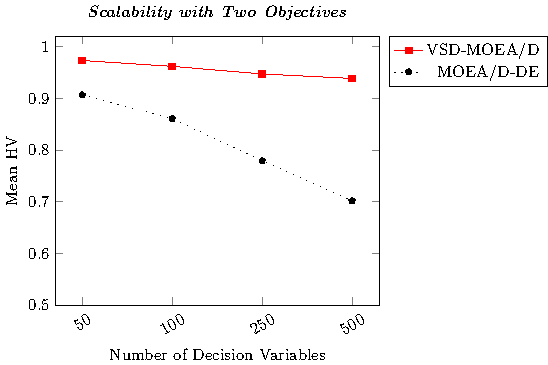
\includegraphics[scale=0.85]{images/Graphic-Scalability-2obj_tikz-figure0.eps}
\caption{Mean of the \HV{} ratio for 35 runs for the two-objective problems considering different numbers of variables}\label{fig:variable-decision-scalability-2obj}
\end{figure}

\begin{figure}[t]
\centering
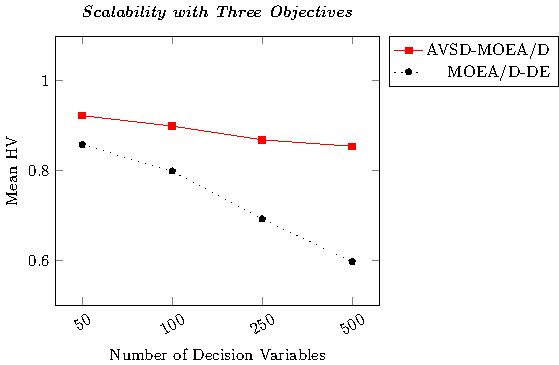
\includegraphics[scale=0.85]{images/Graphic-Scalability-3obj_tikz-figure0.eps}
\caption{Mean of the \HV{} ratio for 35 runs for the three-objective problems considering different numbers of variables} \label{fig:variable-decision-scalability-3obj}
\end{figure}



\section{Conclusion}
\label{Sec:Conclusion}
Premature convergence is one of the most typical drawbacks of \EAS{}.
%
\MOEAS{} indirectly promote the preservation of diversity in the variable space
because of the implicit relationship between the diversity maintained in the objective space and the
one maintained in the variable space.
%
However, for many problems the degree of diversity maintained is not sufficient to ensure the exploratory
power of genetic operators and locate the optimal regions.
%
In single-objective optimization, many of the state-of-the-art algorithms explicitly manage
diversity.
%
Specifically, those schemes that relate the degree of diversity to the elapsed period of execution 
and to the stopping criterion
have excelled.
%
This paper shows that this design principle is also helpful in the area of multi-objective optimization,
where the optimization of many of the most complex popular benchmark problems can be improved further
by applying this design principle.

In order to prove this hypothesis, a novel replacement operator based on the aforementioned design principle
is applied to generate a decomposition-based \MOEA{} that takes into account the diversity in both the variable 
and objective spaces.
%
This is done using a dynamic penalty method. 
%
Note that since the aim of the approach is to improve the results when considering metrics in the objective space,
the importance given to the diversity in the variable space is reduced as the evolution progresses, meaning that
in the later phases, our proposal behaves more similarly to traditional \MOEAS{}.
%
Additionally, taking into account recent advances, and to ensure that our proposal maintains
high-quality solutions despite the penalty scheme, an external archive based on the
R2-indicator is incorporated.
%
Because of this, we refer to our proposal as \textit{Archived Variable Space Diversity MOEA based on Decomposition} (\AVSDMOEAD{}).

The experimental validation carried out shows the remarkable improvement provided by \AVSDMOEAD{} in comparison to
state-of-the-art \MOEAS{} with both two-objective and three-objective problems.
%
The scalability analyses show that as the number of decision variables increases, the benefits of including
proper diversity management are even more important, so the differences in performance increase.
%
In fact, the most remarkable benefits emerge for the most complex cases.
%
Moreover, the analysis of the initial penalty threshold, which is an additional parameter required by \AVSDMOEAD{}, 
shows that the method is quite robust, which makes finding a proper parameter value an easy task.
%
Finally, in order to better understand the reasons behind the huge superiority of our proposal, some analyses involving
the dynamics of the populations are provided.
%
In comparison to state-of-the-art algorithms, our proposal clearly slows down convergence.

In the future, we plan to apply the principles studied in this paper to other categories of \MOEAS{}.
%
For instance, including the diversity management method presented in this paper in indicator-based \MOEAS{} seems plausible.
%
Additionally, in order to obtain even better results, these strategies are going to be incorporated with continuation and/or individual
improvement methods.


\section*{Acknowledgments}
Authors acknowledge the financial support from CONACyT through the ``Ciencia B\'asica'' project no. 285599
and the support from ``Laboratorio de Superc\'omputo del Bajio'' through the project 300832 from CONACyT.


%% The Appendices part is started with the command \appendix;
%% appendix sections are then done as normal sections
%% \appendix

%% \section{}
%% \label{}

%% References
%%
%% Following citation commands can be used in the body text:
%% Usage of \cite is as follows:
%%   \cite{key}          ==>>  [#]
%%   \cite[chap. 2]{key} ==>>  [#, chap. 2]
%%   \citet{key}         ==>>  Author [#]

%% References with bibTeX database:

% \bibliographystyle{model1-num-names}

%% New version of the num-names style
\bibliographystyle{elsarticle-num-names}
\bibliography{bibtex/References.bib}

%% Authors are advised to submit their bibtex database files. They are
%% requested to list a bibtex style file in the manuscript if they do
%% not want to use model1-num-names.bst.

%% References without bibTeX database:

% \begin{thebibliography}{00}

%% \bibitem must have the following form:
%%   \bibitem{key}...
%%

% \bibitem{}

% \end{thebibliography}


\end{document}

%%
%% End of file `elsarticle-template-1-num.tex'.
